\documentclass[a4paper]{book}
\usepackage{feynmanslop}

\title{Fisica}
\author{Zeno Saletti}
\date{\today}


\begin{document}

\begin{titlepage}

\newgeometry{left = 0cm, right = 0cm, top = 0cm, bottom = 0cm}

\begin{figure}
    \pagecolor{brown}\afterpage{\nopagecolor}
    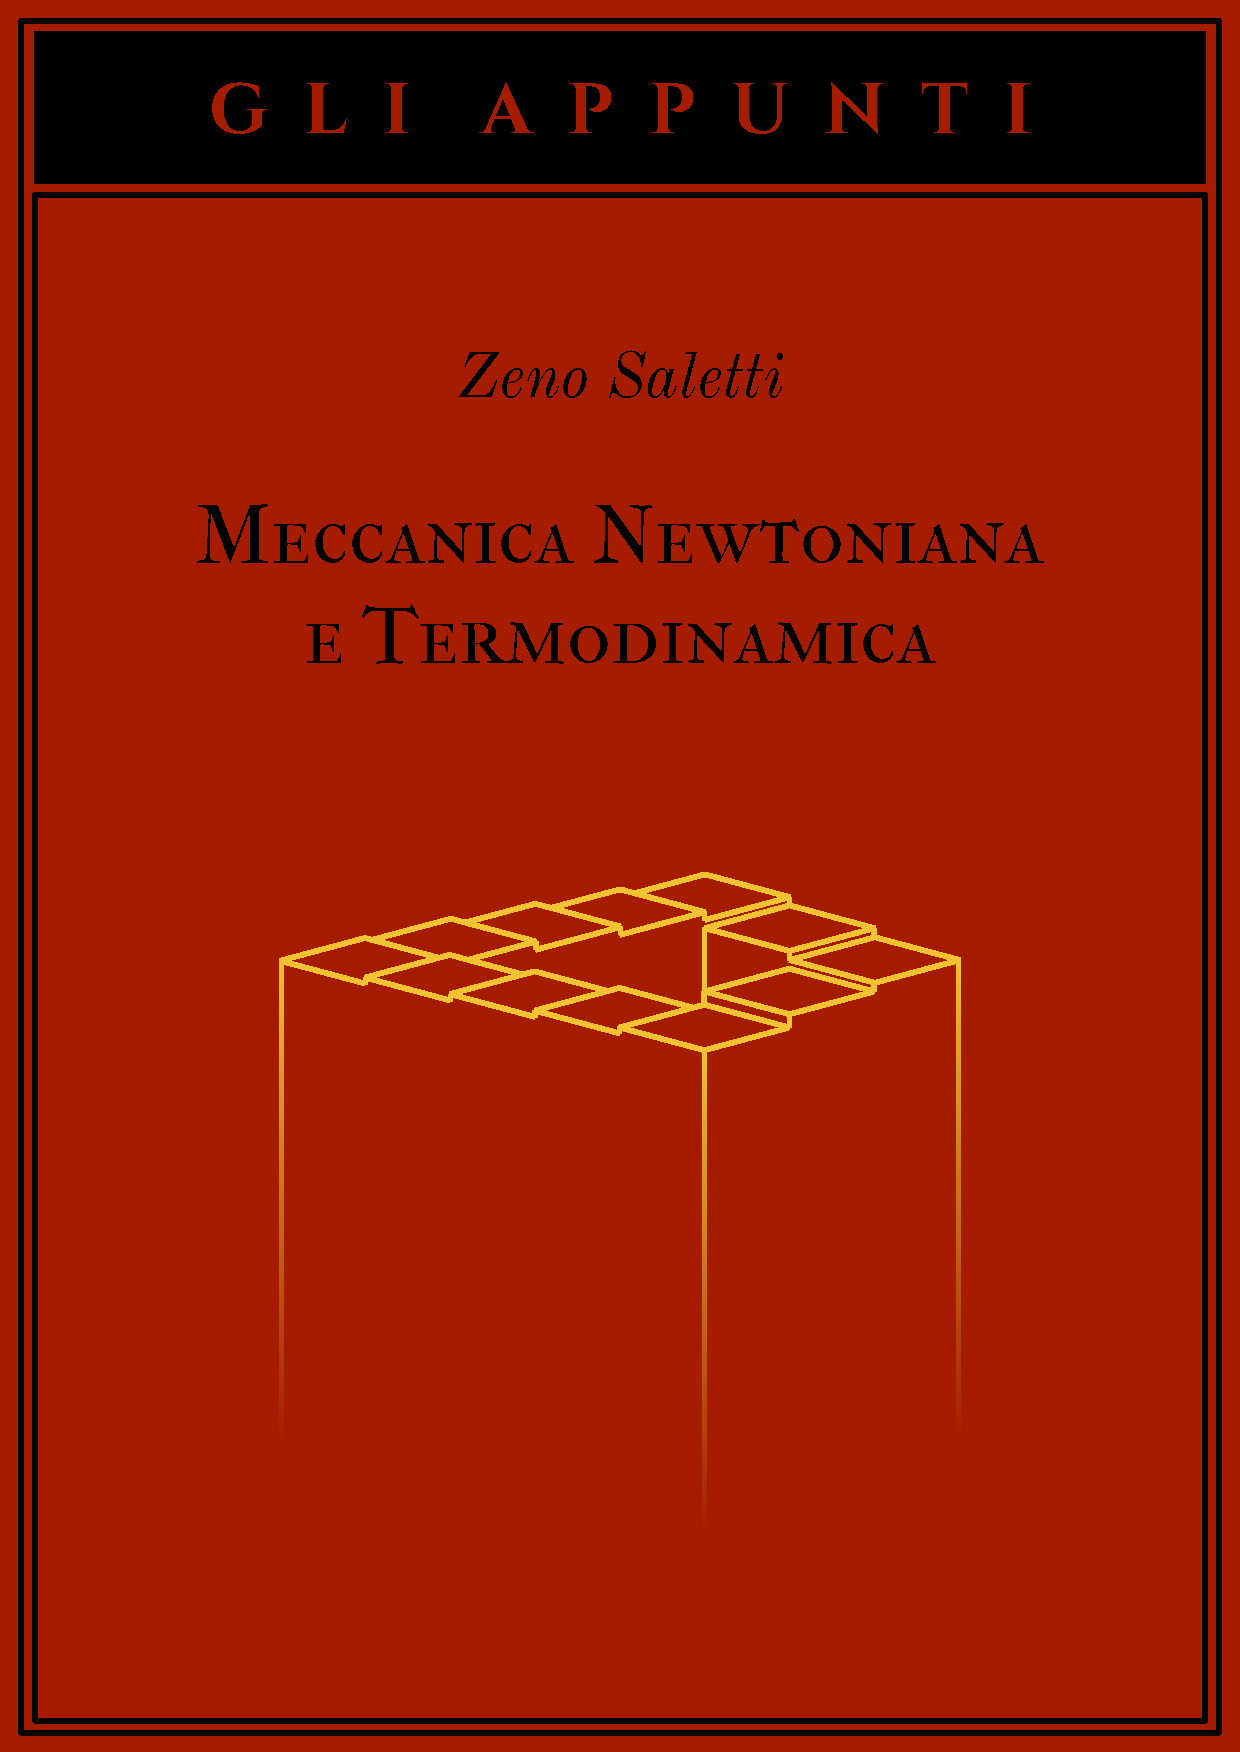
\includegraphics[width = \linewidth]{bookcover.pdf} % also works with logo.pdf
\end{figure}

\restoregeometry

\end{titlepage}
\epigraph{If, in some cataclysm, all of scientific knowledge were
to be destroyed, and only one sentence passed on to the next generations
of creatures, what statement would contain the most information in the
fewest words? I believe it is the \textit{atomic hypothesis} [...]
that \textit{all things are made of atoms—little particles that move
around in perpetual motion, attracting each other when they are a little
distance apart, but repelling upon being squeezed into one another.}
In that one sentence, you will see, there is an enormous amount of
information about the world, if just a little imagination and
thinking are applied.}{Richard P. Feynman,\\\textit{The Feynman Lectures on Physics}\\Vol. I}

\vspace*{5cm}

\begin{center}
    In copertina: \href{https://en.wikipedia.org/wiki/Penrose_stairs}{\textcolor{blue}{\textit{La Scala di Penrose}}}
\end{center}
\begin{center}
    Link alla repository di questo progetto: \href{https://github.com/zenosaltt/phy}{\faGithub \space \textcolor{blue}{\texttt{github.com/zenosaltt/phy}}}
\end{center}

\vspace*{4cm}

\begin{center}
Consigliamo di consultare questa dispensa ascoltando il brano seguente:\\
\href{https://www.youtube.com/watch?v=JuSsvM8B4Jc}{\textcolor{blue}{\textit{Cornfield Chase} by Hans Zimmer (from \textit{Interstellar} by Christopher Nolan)}}
\end{center}
\chapter*{}

\vspace*{0.2\paperheight}
\begin{center}
    \textcolor{red}{\textbf{\Huge Avvertenze!}}\\
    \begin{center}
    
    \end{center}
    Questa è una raccolta di appunti redatta da studenti e indirizzata
    ad altri studenti. Essa non pretende di essere un libro
    di testo, ma unicamente una forma di aiuto libero e gratuito per coloro
    che sono in cerca di materiale per il supporto allo studio.
    Pertanto, si raccomanda di non preparare l'esame basandosi esclusivamente
    su questi appunti, ma di fare riferimento alle lezioni frontali
    e ai libri (in breve, a chi è esperto in merito). Qualora quindi
    vi fossero affermazioni fuorvianti o false contenute in queste
    pagine, \textit{gli autori non si assumono la responsabilità di eventuali
    esiti (1) non corrispondenti alle aspettative oppure (2) negativi di esami
    o altre forme di prove ufficiali presso l'Università}; gli autori sono anzi
    aperti a eventuali segnalazioni e correzioni volte al miglioramento
    dell'esposizione.

    Prima che eventuali eruditi procedano a lamentarsi o
    a stilare critiche degne di una giuria del premio
    Strega, precisiamo che questi appunti sono stati realizzati
    da studenti di informatica e pensati per studenti di informatica,
    con conoscenze basilari di \LaTeX.
    Ci auguriamo che i fisici non stiano facendo affidamento su
    queste pagine per integrare lo studio.
\end{center}

%\newpage
%\input{./matter/frontmatter/pre.tex}

\newpage
\section*{Errata}
È statisticamente difficile, se non impossibile, produrre un testo
privo di errori. Questi appunti non sono un'eccezione.
Spieghiamo di seguito come e cosa si può segnalare.

\subsubsection*{Come segnalare}
\begin{itemize}
    \item Se conosci (o non conosci) gli autori, contattandoli o cercandoli direttamente in Università
    o su canali di comunicazione come Telegram o E-Mail istituzionale
    (\texttt{<nome>.<cognome>@studenti.unitn.it}).

    \item Se conosci GitHub, aprendo una \href{https://github.com/zenosaltt/phy/issues}{\textcolor{blue}{issue(\faGithub)}} sulla repository del progetto.

    %\item Se conosci GitHub e in più \LaTeX\@, mettendo mano direttamente al codice
    %e proponendo delle modifiche mediante una pull request.
\end{itemize}

\subsubsection*{Cosa segnalare}
Per semplicità e chiarezza, dividiamo gli errori in categorie, ordinandoli secondo una priorità decrescente:

\begin{itemize}
    \item Errori grammaticali, lessicali, sintattici e tutti quegli errori nell'impiego
    del linguaggio che ostacolano la comprensione del testo.

    \item Nozioni che non corrispondono al vero o incomplete, di qualsiasi genere (ma
    attinenti alla materia trattata in queste pagine):
    leggi mal formulate; affermazioni, supposizioni, definizioni imprecise, false o
    superficiali\footnote{Sono ovviamente contemplate correzioni e integrazioni da parte di appasionati
    o esperti in campi specifici: la meccanica dei motori termici descritta brevemente
    nel capitolo di termodinamica, storia e filosofia, balistica e molto altro ancora.}; affermazioni false
    relative a fatti o persone reali.

    \item Errori di calcolo o risultati errati nelle equazioni e negli esempi del testo e negli
    esercizi dell'appendice.

    \item Irregolarità nell'utilizzo di notazioni standard, come i simboli matematici
    o la citazione di testi.

    \item Link malfunzionanti.
    
    \item Altri errori di battitura oppure grafici ed estetici.
\end{itemize}

Vengono contemplati con riguardo anche eventuali miglioramenti o integrazioni,
qualora il tempo e le energie a disposizione lo permettano:

\begin{itemize}
    \item Esercizi.
    \item Immagini che arricchiscono il testo e stimolano la comprensione.
    \item Rivisitazioni dell'ordine dei capitoli, delle sezioni, dei paragrafi.
    \item Rivisitazione del design e della veste grafica.
    \item Approfondimenti inerenti agli argomenti affrontati nel corso.
\end{itemize}

\subsubsection*{Tempi}
A seconda del numero di segnalazioni, della mole di lavoro che queste
comportano e dell'intervallo di tempo e dell periodo dell'anno nei quali
esse vengono inviate, i tempi di aggiornamento possono variare. Non
garantiamo correzioni tempestive, ma ci impegneremo ad elaborarle in
futuro.
\section*{Riconoscimenti}
Questi appunti non sono stati realizzati dal nulla.
Alcuni materiali di supporto sono stati impiegati
per portare alla luce queste pagine.

\subsubsection*{Testi}
Gran parte del testo è una trascrizione in linguaggio tipografico \LaTeX\@
degli appunti reperiti durante
il corso di Fisica (a.a. 2023-2024) tenuto dal prof. Roberto Iuppa, presso
l'Università degli Studi di Trento. Organizzazione e ordine dei
capitoli ricalcano la successione delle lezioni frontali, con alcune
rivisitazioni dell'ordine di esposizione degli argomenti.

Di grande ispirazione e supporto sono stati:
\begin{itemize}
    \item R. P. Feynman, R. B. Leighton, M. Sands. \textit{The Feynman Lectures on Physics. Volume I: Mainly Mechanics, Radiation, and Heat}. Addison-Wesley. 1964.
    \item J. Walker. \textit{Dalla Meccanica alla Fisica Moderna. Meccanica - Termodinamica}. Pearson (edizione italiana). 2012.
\end{itemize}

\subsubsection*{Immagini}
Tutte le immagini che si trovano in questi appunti sono state realizzate
integralmente a mano, incluso il design di copertina, utilizzando
lo strumento Disegni della suite Google. Tutte le risorse
grafiche vettoriali di questo testo sono incluse nella repository del progetto.

\subsubsection*{Esercizi}
Gli esercizi proposti sono una selezione di problemi
giudicati interessanti o
di importanza basilare, perché incorporano principi chiave studiati nel corso.
Questi esercizi sono stati reperiti dai libri di testo citati precedentemente
e da fogli relativi ad esercitazioni dell'anno accademico corrente (a loro
volta raccolti dal Web), più alcuni testi d'esame antecedenti l'anno accademico
nel quale questa dispensa è stata redatta per la prima volta. Questi testi
d'esame sono stati pubblicati dal professore stesso sul canale Moodle del corso.

\chapter*{Guida al testo}
Saremo onesti e concisi: questi appunti sono lunghi e prolissi.
Ma alcuni aspetti sono stati curati per soddisfare le esigenze di
coloro che intendono solo dare rapide occhiate alle nozioni di rilievo
in questo corso.

\begin{itemize}
    \item \textit{Indice}: l'indice è la prima arma a portata di studenti che intendono
    consultare rapidamente gli appunti. Ci siamo impegnati al meglio per rendere
    concisi i titoli di capitoli e sezioni per raggiungere questo scopo. L'indice
    contiene collegamenti cliccabili che conducono direttamente alla pagina selezionata.

    \item \textit{Microindici}: all'inizio di ogni capitolo viene collocato un microindice
    contenente la lista di macrosezioni, visibile nel margine destro. Anche questi microindici
    sono dotati di collegamenti interni alle rispettive pagine del testo.

    \item \textit{Box colorati}: definizioni, leggi e principi notevoli sono risaltati da box colorati.
    
    \item \textit{Equazioni etichettate}: se non evidenziate dai box, le leggi e altri
    risultati (per lo più matematici) rilevanti sono comunque numerati tra
    parentesi tonde.

    \item \textit{Appendici (in sviluppo...)}: vengono anche curate alcune appendici
    che riportano risorse utili di svariato genere, quali un piccolo compendio di esercizi,
    le leggi fisiche rilevanti in questo corso e altro ancora. L'indice riporta anche
    queste appendici.
\end{itemize}

Per coloro che invece manifestano maggiore interesse per questa scienza, alcuni
capitoli includono approfondimenti che possono stuzzicare menti impavide (anche
se non sono di certo questi appunti a contenere tutti quelli più interessanti,
qui troverete solo un minimo assaggio). Gli approfondimenti non sono
indispensabili per questo corso.

\section*{Requisiti}
Seppur superficialmente, questi appunti coprono un'ampia area della fisica
e il substrato matematico necessario alla sua comprensione è piuttosto eterogeneo.
Anche se non sarà sempre necessario ricordare tutto,
questi appunti presuppongono conoscenze di: analisi matematica (derivazione,
integrazione), trigonometria, geometria analitica (sistemi di assi
cartesiani e calcoli annessi) geometria e algebra lineare (vettori,
sistemi di equazioni). Conoscenze matematiche più avanzate
sono di aiuto ma non strettamente necessarie.

\section*{Sulla notazione}
Si utilizzano spesso in questo testo notazioni matematiche compatte.
Invitiamo il lettore a consultare l'appendice dei simboli per eventuali
chiarimenti. I testi potrebbero non essere esenti da abusi di notazione\footnote{Scusateci tanto
ma il font AMS è talmente bello che è facile perdere il controllo scrivendo
appunti in \LaTeX.}.

%Un intero capitolo di approfondimento contiene argomenti
%relativi all'Elettromagnetismo, non più mostrato, come un tempo, durante
%l'anno accademico attuale (2023/2024).

\dominitoc %otherwise tocs won't appear (but in linux it is not necessary, apparently)
\tableofcontents

\chptr{Introduzione alla Fisica}
\marginpar{\minitoc}

\section{Definizione e scopi della fisica}

Si possono formulare definizioni diverse riguardo la disciplina scientifica
della fisica, come la seguente:

\vspace{8pt}
\begin{tcolorbox}[colback = yellow!30, colframe = yellow!30!black, title = {Fisica}]
La fisica è lo studio quantitativo delle leggi fondamentali della natura, cioè
delle leggi che governano tutti i fenomeni naturali dell'universo.

Una legge fisica (o principio) è una regolarità della natura esprimibile in forma
matematica, ma anche una verità non dimostrabile che tuttavia non contraddice i
fenomeni osservabili dell'esperienza.
\end{tcolorbox}
\vspace{5pt}

\noindent La fisica si avvale del \textit{metodo sceintifico}, secondo cui la natura deve
essere interrogata per vie sperimentali, facendosi guidare da \textit{ipotesi} e
modelli teorici. Una particolarità di questo metodo è la capacità di isolare
un certo fenomeno che si intende studiare, tralasciando (si userà spesso il
termine \textit{trascurare}) certi aspetti ritenuti non rilevanti in modo da
scoprire quelle regolarità dalle quali potrebbe essere dedotta una certa
relazione matematica.

Il ruolo della matematica è quello di fornire un linguaggio formale per descrivere
quantitativamente i fenomeni osservati e costruire modelli utili alla loro
trattazione.



\section{Grandezze fisiche}
La fisica è una scienza quantitativa, ovvero essa si occupa di caratteristiche
e proprietà del reale che possono essere misurate e quantificate: Le cosiddette
grandezze fisiche. Esempi di grandezze fisiche sono la lunghezza, la massa, la
temperatura, la durata temporale e così via.

\vspace{8pt}
\begin{tcolorbox}[colback = yellow!30, colframe = yellow!30!black, title = {Grandezza fisica}]
Una grandezza fisica è una caratteristica di un oggetto o di un fenomeno che può
essere misurata in termini quantitativi (oltre che oggettivi, ovvero indipendentemente
dalle sensazioni personali degli individui).
\end{tcolorbox}
\vspace{5pt}

\noindent È implicito, intuitivamente, il concetto di \textit{misura}. Misurare una grandezza
fisica significa confrontarla con una grandezza ``campione'', detta \textit{unità
di misura}, e stabilire quante volte l'unità è contenuta nella
grandezza data. Il valore numerico ottenuto è la misura della grandezza e deve
essere sempre accompagnato dall'unità scelta.
In altre parole, la \textit{misura} non è altro che un \textit{rapporto} tra la
grandezza che si intende misurare e la grandezza campione scelta convenzionalmente
per tale scopo.

Mostriamo un esempio: supponiamo di voler misurare la lunghezza di qualsiasi cosa
in ``chiavette USB'' (si potrebbe argomentare circa quale chiavetta si stia
impiegando e quale posizione la chiavetta debba assumere durante la misura.
Supponiamo qui che la chiavetta sia posta in verticale, senza perderci in ulteriori
dettagli). Decidiamo poi di misurare l'altezza di una porta—anche qui, non
specifichiamo quale porta—utilizzando l'unità appena scelta. Supponiamo quindi
di aver registrato il seguente dato:
\[ H = 20 \text{ chiavette USB} \]
Notare come siano stati specificati:
\begin{itemize}
    \item Un nome per l'oggetto che si intendeva misurare, $H$, ovvero l'altezza
    della porta.
    \item Il valore numerico individuato, 20.
    \item Una affermazione per legare il nome e il dato, = (``corrisponde a'', ``è
    uguale a'')—caratteristica che peraltro si trova anche nei linguaggi di
    programmazione. Si presti bene attenzione che l'uguaglianza matematica
    non implica a priori l'equivalenza fisica. Questa sottigliezza si
    noterà bene nella formulazione del principio zero della termodinamica.
    \item L'unità di misura, chiavette USB.
\end{itemize}
Tuttavia, tale misurazione non è stata affatto sincera: non vi è la
garanzia che il valore registrato sia esatto. La prossima sezione
tratterà questo problema, ovvero quello dell'\textit{incertezza}.


\section{Incertezza}
Idealmente, si vorrebbe impiegare, grazie alle misure, numeri puntuali ed esatti.
In altre parole, dei numeri con una precisione indefinita, aventi un numero
illimitato di cifre decimali e non.

Ma quando si effettua una misura di una grandezza, il risultato ottenuto è noto solo
con una certa precisione. Riprendendo l'esempio della chiavetta USB, è impossible
misurare con certezza tutte le lunghezze, in quanto non multipli esatti della
chiavetta stessa: ci sarà sempre un certo margine di ``un pezzo di chiavetta'',
minore dell'unità prescelta. Ma al di sotto di quella unità non è possibile
fornire alcuna garanzia sulla puntualità del dato. In altre parole, la
\textit{sensibilità}\footnote{La più piccola variazione della grandezza che lo
strumento è in grado di rilevare.} dello strumento è uno dei limiti alla precisione
della misura.

\vspace{8pt}
\begin{tcolorbox}[colback = yellow!30, colframe = yellow!30!black, title = {Cifre significative del risultato di una misura}]
Le cifre significative del risultato di una misura sono le cifre note
con certezza e la prima cifra incerta. In altre parole, esse sono le cifre che si
possono controllare con lo strumento impiegato nella misura.
\end{tcolorbox}
\vspace{5pt}

\noindent Ad esempio, il valore corrispondente alla lunghezza di una barca $L = 10.5$ m
possiede tre cifre significative, che non equivale a $10.50$ m. Il secondo dato,
infatti, dichiara che la misurazione è stata possibile controllando le cifre
fino al centimetro. $L = 0.002$ possiede solo una cifra significativa, perché
in genere si ignorano gli zeri a sinistra della prima cifra significativa diversa
da zero. Possono essere ambigui valori come $L = 2500 \text{ m}$: Quali zeri sono
cifre significative? Chi ha compiuto la misura può aver utilizzato un'asta lunga
un centinaio di metri, dunque non è possibile stabilire il valore delle cifre
meno significative delle centinaia. Come vedremo tra poco, è utile esprimere questi valori in
notazione scientifica per eliminare ambiguità.

Vi potrebbero anche essere errori dovuti a imprecisioni introdotte nell'utilizzo
degli strumenti di misura. Questo errore deve tuttavia essere quantificato ed ogni
misura ne è affetta (comprese quelle che non la riportano).

\vspace{8pt}
\begin{tcolorbox}[colback = yellow!30, colframe = yellow!30!black, title = {Risultato della misura di una grandezza}]
Il risultato della misura di una grandezza è sempre un'approssimazione
accompagnata da una certa incertezza, ovvero un \textbf{valore attendibile}
e un \textbf{errore assoluto} (o semplicemente \textit{incertezza}).
\[ x = \overline{x} \pm e_x  \]
\end{tcolorbox}
\vspace{5pt}

Questo risultato non è quindi altro che un intervallo in cui il valore reale
della misura si trova. Ci limiteremo agli errori relativi a singole misure,
nelle quali $x$ corrisponde al valore misurato e $e_x$ la sensibilità dello
strumento\footnote{Gli errori si propagano tuttavia anche durante i calcoli,
secondo definizioni che tuttavia non verranno affrontate.}. Di conseguenza, possiamo ora correggere il risultato della misura
effettuata in chiavette USB:

\[ H = (20 \pm 1) \text{ chiavette USB} \]

\section{Notazione scientifica}
Unità di misura come il metro e il kologrammo sono comode nella vita di tutti i
giorni, ma rappresentano quantità enormi su scala atomica e subatomica e quantità
minuscole su scala astronomica e cosmica. Conseguenza di ciò è che alcune misure
possono essere espresse da numeri ``scomodi''. Considerando solo valori attendibili,
la massa dell'atomo di idrogeno è circa
\[ m_H = 0,000 000 000 000 000 000 000 000 001 67 \text{ kg} \]
mentre la massa della Terra è
\[ m_T = 5 970 000 000 000 000 000 000 000 \text{ kg} \]
È pressoché evidente il motivo di tale scomodità: La notazione è di difficile
trattazione. Viene dunque in aiuto la \textbf{notazione scientifica}, ovvero una
notazione numerica che permette di contrarre rappresentazioni estese impiegando
potenze di 10. Nella notazione scientifica, ogni numero è scritto come prodotto
di due fattori:
\begin{itemize}
    \item Un numero decimale $x:x\in \mathbb{R}, 1\leq x < 10$[\footnote{In realtà, questa notazione corrisponde alla variante ``ingegneristica''. Esiste anche una notazione che prevede che il valore espresso $x$ sia $0\leq x < 1$.}].
    \item Una potenza di 10, con esponente intero.
\end{itemize}
Pertanto, le misure precedenti si possono esprimere in notazione scientifica come
segue:
\[ m_H = 1,67 \cdot 10^{-27} \text{ kg} \]
\[ m_T = 5,97 \cdot 10^{24} \text{ kg}\]
Notare come la notazione sia in grado di eliminare ambiguità sul numero di cifre
significative: ora sappiamo che la massa della Terra è stata calcolata fino a
tre cifre significative e non 25.

Non sempre è necessario calcolare esattamente il valore di una certa grandezza.
Talvolta basta averne solo un'idea approssimata. Supponiamo, ad esempio, che sia
sufficiente sapere se una certa massa vale all'incirca 1 grammo oppure 1
ettogrammo. In questo caso, possiamo accontentarci di stimare il valore della
massa con un'accuratezza di un fattore 10, cioè di calcolare il suo ordine di
grandezza.

\vspace{8pt}
\begin{tcolorbox}[colback = yellow!30, colframe = yellow!30!black, title = {Ordine di grandezza}]
L'ordine di grandezza di un numero è la potenza di 10 più vicina a quel numero.
\end{tcolorbox}
\vspace{5pt}

\noindent Per determinare l'ordine di grandezza di un numero occorre quindi esprimerlo in
notazione scientifica—prodotto di un numero decimale compreso tra 1 e 10 e di
una potenza di 10—e poi approssimare il valore alla potenza di 10 più vicina.
In particolare:
\begin{itemize}
    \item Se il numero decimale è minore di 5, si mantiene l'esponente della
    potenza. Ad esempio:
    \[ 3,6 \cdot 10^2 \to \text{ Ordine di grandezza } 10^2 \]
    \[ 4,2 \cdot 10^{-3} \to \text{ Ordine di grandezza } 10^{-3} \]

    \item Se il numero decimale è maggiore di 5, si somma +1 all'esponente della
    potenza. Ad esempio:
    \[ 9 \cdot 10^2 \approx 10 \cdot 10^2 \to \text{ Ordine di grandezza } 10^3 \]
    \[ 8,1 \cdot 10^{-12} \approx 10 \cdot 10^{-12} \to \text{ Ordine di grandezza } 10^{-11} \]
\end{itemize}

\noindent Sono stati definiti dei prefissi stadard per certi ordini di grandezza notevoli,
cioè quelli che, escludendo la potenza nulla, rappresentano multipli di tre.
\marginpar{
\footnotesize
%\hspace*{-0.5cm}
\begin{tabular}{c|c|c}
    Potenza   & Simbolo & Prefisso\\
    \hline
    $10^{12}$  & T       & Tera\\
    $10^{9}$   & G       & Giga\\
    $10^{6}$   & M       & Mega\\
    $10^{3}$   & k       & kilo\\
    $10^{-3}$  & m       & milli\\
    $10^{-6}$  & $\mu$   & micro\\
    $10^{-9}$  & n       & nano\\
    $10^{-12}$ & p       & pico\\
\end{tabular}
}
Utilizzando questi prefissi, di fianco all'unità di misura adottata, si contrae
ancora di più la notazione scientifica, sottointendendo un certo ordine di
grandezza.
\chptr{Descrizione del moto}
\marginpar{\minitoc}

\section{Moto del punto materiale}
Un corpo è in moto quando la sua posizione nello spazio cambia nel tempo.
Supponiamo di voler descrivere il moto di un'auto, in particolare la sua
velocità approssimativa, ovvero la distanza che essa percorre in una certa unità di
tempo. Sappiamo che la macchina ha una certa estensione, ovvero è
voluminosa. Se essa deve percorrere un kilometro, la sua lunghezza,
altezza e larghezza sono praticamente ininfluenti (trascurabili) ai fini della misura
grossolana che vogliamo effettuare. Se però vogliamo calcolare la velocità
percorrendo un metro, è probabile che l'auto scelta sia ben più lunga
di quella distanza. Bisogna quindi stabilire quale sia la posizione
dell'auto.

In questo corso, assumiamo che la posizione di qualsiasi oggetto sia
in realtà la posizione di un suo punto, il cosiddetto punto materiale.
Nell'auto, per esempio, misureremmo in realtà la velocità della punta
del suo cofano, oppure di un punto sul fanalino posteriore sinistro.
Il punto si chiama ``materiale'' perché il punto che identifica la
posizione concentra in sé anche tutta la massa dell'oggetto che esso
rappresenta, come ad esempio l'auto, che è un oggetto esteso,
voluminoso. Le sue dimensioni sono per noi trascurabili rispetto
a quelle dell'ambiente in cui osserviamo il moto.


\section{Il piano spazio-tempo}

\section{Moto in una dimensione}
\subsection{Moto rettilineo uniforme}
\subsection{Moto rettilineo uniformemente accelerato}

\section{Altri moti}
\subsection{Moto in più dimensioni}
\subsection{Moto circolare uniforme}
\subsection{Moto armonico semplice}


\subsection*{Sistemi di riferimento}
Abbiamo detto che il moto è caratterizzato da un cambiamento di posizione. Il primo
passo nella descrizione del moto di un corpo consiste quindi nello stabilire il
modello da adottare per catturare il concetto di \textbf{posizione}. Sappiamo già
che i modelli della fisica si basano sul linguaggio matematico; il modello più
naturale che si possa adottare è dunque un sistema di assi cartesiani. Da qui, la
posizione del corpo può essere specificata mediante coordinate. Una speciale
coordinata è il tempo (in caso di moti in più di una dimensione spaziale, il
tempo viene spesso omesso dalla rappresentazione grafica).

\begin{marginfigure}
    \centering
    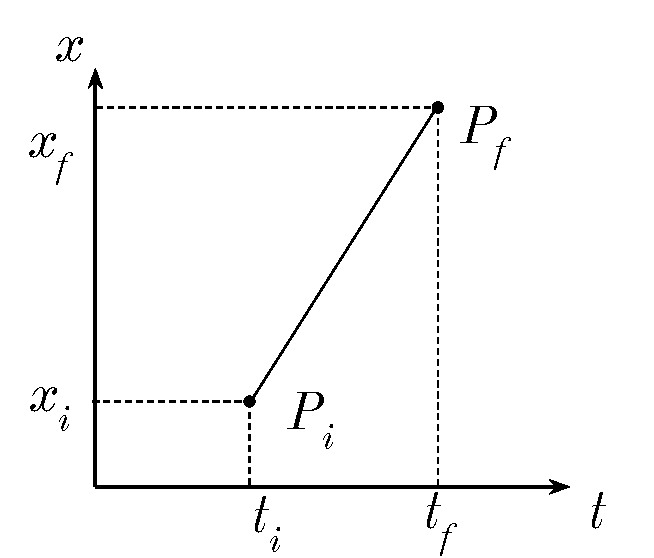
\includegraphics[width = \marginparwidth]{punto_sul_cartesiano.pdf}
    \caption{Sistema di riferimento con una sola dimensione spaziale ($x$)
    in funzione del tempo ($t$). All'istante $t_i$, il punto materiale $P$
    si trova nella posizione $x_i$}
    \label{point}
\end{marginfigure}

La scelta del sistema di riferimento di assi cartesiani è del tutto arbitraria\footnote{
Gli assi possono addirittura non essere ortogonali, purché si segua la \textit{regola del
parallelogramma} e si rinunci alle proprietà e alle regolarità matematiche degli
assi ortogonali, come il teorema di Pitagora per il calcolo del modulo dei
vettori.}, ma una volta fissata è necessario essere coerenti con essa.
Questo permette di riflettere sul fatto che il moto è sempre relativo al sitema di
riferimento adottato: cambiando sistema di riferimento, il moto cambia.

Fissando gli assi cartesiani, si fissa una componente di un \textit{sistema di
riferimento}. Intuitivamente, un sistema di riferimento è il ``punto di vista''
da cui si sceglie di effettuare misure ed osservazioni riguardo ad un certo
fenomeno.

\subsection*{Posizione e traiettoria}
Alla base della descrizione del moto, è importante individuare quelli che sono
chiamati \textit{posizione} e \textit{traiettoria}. Avendo assunto la semplificazione
del punto materiale, è intuibile che la posizione verrà descritta matematicamente
come una tupla di coordinate inserite in un sistema di assi cartesiani. Tra le
coordinate, è importante tenere presente anche il tempo. Di fatto, abbiamo
introdotto il moto definendolo come variazione della posizione nel tempo.

La traiettoria non è altro che la linea che unisce le posizioni occupate
successivamente dal corpo. Tratteremo prima moti con traiettorie rettilinee,
per poi passare a traiettorie curvilinee semplici, come il moto circolare.

\begin{tcolorbox}[colback = yellow!30, colframe = yellow!30!black, title = {Posizione e traiettoria}]
\begin{itemize}
    \item La posizione di un corpo è il punto nel quale esso si trova entro un
    determinato sistema di riferimento.

    \item La traiettoria di un corpo è l'insieme di posizioni occupate da esso
    durante il suo moto.
\end{itemize}
\end{tcolorbox}

\subsection*{Distanza e spostamento}
Durante il moto, è possibile registrare la \textbf{distanza} percorsa
dall'oggetto e il suo \textbf{spostamento}. Il primo è una grandezza
scalare e corrisponde alla distanza totale percorsa durante il tragitto
effettuato dall'oggetto in moto. Il secondo è una grandezza vettoriale e
corrisponde al cambiamento di posizione,
cioè la differenza tra la posizione iniziale e quella finale dell'oggetto:
\[ \Delta \mathbf{x} = \mathbf{x}_f - \mathbf{x}_i \]

\section*{Interpretazioni geometriche}

\begin{marginfigure}
    \centering
    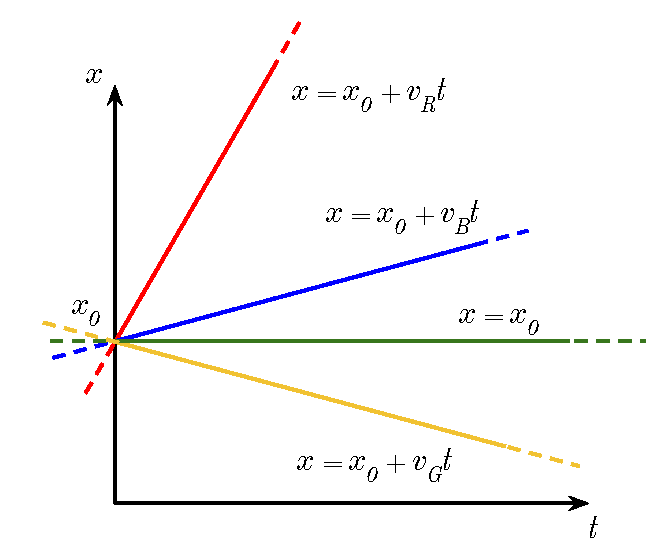
\includegraphics[width = \marginparwidth]{velocita_come_pendenza.pdf}
    \caption{Oggetti in moto rettilineo uniforme con velocità differenti}
\end{marginfigure}




\section*{Moto circolare}
Cambiamo ora la traiettoria dell'oggetto in moto, considerando quella circolare.
Per descrivere un moto circolare è conveniente impiegare coordinate differenti,
dette polari. Fissando il centro di un piano cartesiano al centro di una
circonferenza di raggio $r$, possiamo identificare la posizione di ogni punto
della circonferenza con la coppia $(r, \theta)$, dove $\theta$ è l'angolo
formato dalla semiretta appartenente al sistema di riferimento e dalla semiretta
che interseca la circonferenza nel punto desiderato (entrambe le semirette
hanno origine nel centro del piano cartesiano, quindi della circonferenza).

\begin{marginfigure}
    \centering
    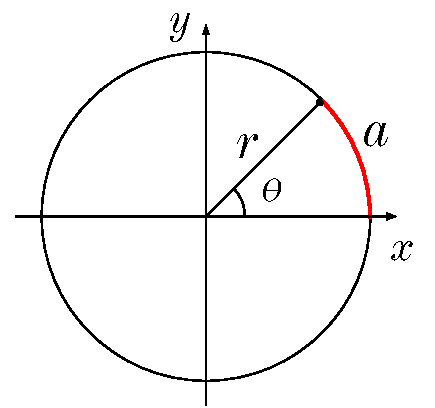
\includegraphics[width = \marginparwidth]{moto_circolare.pdf}
    \caption{Sistema di riferimento per un moto circolare.}
    \label{circref}
\end{marginfigure}

Assumeremo qui che $r$ non varia durante il moto. Per questo, viene omessa
la coordinata $r$ e si considera invece la posizione derivante da $\theta$,
detta anche \textit{posizione angolare}. Convenzionalmente, $\theta > 0$ se
misurato in senso antiorario a partire dall'asse di riferimento (come in
Figura \ref{circref}). Si utilizzano inoltre i \textit{radianti} per misurare
$\theta$. I radianti tornano infatti comodi, perché permettono di semplificare
le relazioni tra le grandezze in gioco durante il moto circolare. Innanzitutto,
dato l'arco $a$ in Figura \ref{circref}, vale la relazione \[ a = r\theta \]
Di fatto, la lunghezza totale della circonferenza corrisponde a $C = 2\pi r$,
dove $2\pi$ corrisponde ad un angolo giro espresso in radianti.

\subsection*{Velocità angolare e velocità tangenziale}
Studiamo ora il cambiamento della posizione angolare nel tempo. Come per il
moto rettilineo, possiamo considerare il rapporto tra lo spostamento angolare
e l'intervallo di tempo trascorso. Da qui, si ottiene la velocità angolare:
\[ \omega = \frac{d\theta}{dt} \]
In ogni istante, una particella in moto circolare si muove in direzione
tangenziale alla traiettoria.
\begin{marginfigure}
    \centering
    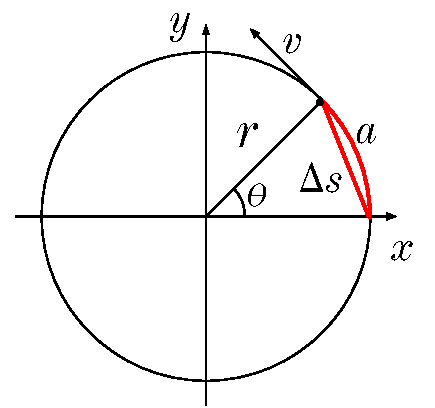
\includegraphics[width = \marginparwidth]{velocita_tangenziale.pdf}
    \caption{Velocità tangenziale.}
    \label{circspeed}
\end{marginfigure}
È chiaro che la particella, muovendosi, copre una certa distanza sulla
circonferenza in un dato intervallo di tempo. Possiamo quindi affermare
che essa ha una velocità, detta \textit{tangenziale}, $v$, oltre che
quella angolare $\omega$. Cerciamo una relazione tra esse: supponiamo che
la particella effettui, in un intervallo infinitesimo $\Delta t$, uno
spostamento angolare altrettanto piccolo $\Delta\theta$ come mostrato in
Figura \ref{circspeed}. Lo spostamento $\Delta s$, dato dalla corda che
sottende l'angolo $\Delta\theta$, approssima l'arco $a = r\Delta\theta$. Quindi:
\[ v = \lim_{\Delta t \to 0}\frac{\Delta s}{\Delta t} = \lim_{\Delta t \to 0} \frac{r\Delta\theta}{\Delta t} = r\lim_{\Delta t \to 0}\frac{\Delta\theta}{\Delta t} = r\omega \]
Abbiamo quindi ottenuto la relazione cercata:
\[ v = r\omega \]
Notare come $v\propto r$, al contrario di $\omega$. Ciò significa che,
assumendo una velocità angolare costante, la velocità tangenziale è tanto
maggiore quanto più $r$ cresce.

\subsection*{Moto circolare uniforme}
Un moto circolare uniforme è un moto circolare con velocità \textit{angolare} costante.
Le regolarità di questo tipo di moto permettono di studiare altre grandezze
importanti per il moto circolare: periodi e accelerazioni.

\subsubsection*{Periodo e frequenza}
La particolarità di questo moto è la sua periodicità, perché esso si ripete
ciclicamente nel tempo. In particolare, un oggetto torna ad occupare la medesima
posizione iniziale dopo un certo intervallo di tempo, chiamato \textbf{periodo} ($T$):
in altre parole, il tempo necessario per compiere ``un giro (ciclo) completo''.
Nel nostro caso, un giro completo corrisponde all'intera circonferenza $C = 2\pi$.
Sapendo che $\omega = \frac{d\theta}{dt}$, è immediato ricavare il periodo:
\[ T = \frac{2\pi}{\omega} \]
Si impiega spesso anche la \textbf{frequenza}, che corrisponde al reciproco
del periodo:
\[ f = \frac{1}{T} \]
L'unità di misura è l'\textit{Hertz} (Hz), ovvero ``cicli al secondo'' (s$^{-1}$),
quindi il numero di cicli compiuti nell'unità di tempo.

\subsubsection*{Accelerazione centripeta}
Riprendendo la prima legge della dinamica, sappiamo che un corpo permane nel
suo stato di moto rettilineo uniforme a meno dell'intervento di agenti esterni.
Nel caso dell'intervento di tali agenti, si osserva un'accelerazione
dell'oggetto, ovvero un cambiamento del suo stato di moto e dunque della sua
velocità. Non viene specificato se questo cambiamento avviene al \textit{modulo}
oppure alla \textit{direzione} della velocità. Infatti, la velocità è una
grandezza vettoriale e una variazione di anche una sola delle sue caratteristiche
comporta un'accelerazione. Per questo motivo, nonostante il modulo della velocità
tangenziale di un corpo in moto circolare uniforme sia costante, la direzione
del suo vettore cambia.

Vi è però il problema aperto di trovare l'agente esterno (la forza) che
mantiene l'oggetto (dotato di massa) nella traiettoria del suo moto circolare.
Esso può essere di varia natura: la tensione di una corda attaccata ad una
pallina che viene fatta roteare; la forza di gravitazione universale che
mantiene in orbita (assumiamo circolare) un pianeta intorno ad un sole; la forza
elettrica che mantiene un elettrone vicino al nucleo (secondo un modello classico
dell'atomo).

Vista quindi l'esistenza di un'accelerazione determinata da un agente esterno,
rimane da capire come è fatto il suo vettore (modulo, verso e direzione).
L'esperienza ci dice che questa accelerazione: (1) cresce con l'aumentare della
velocità angolare; (2) è diretta verso il centro della circonferenza. Ma come
dimostrarlo formalmente per tutti i moti circolari uniformi? Consideriamo la
situazione in Figura \ref{circolare}.
\begin{marginfigure}
    \centering
    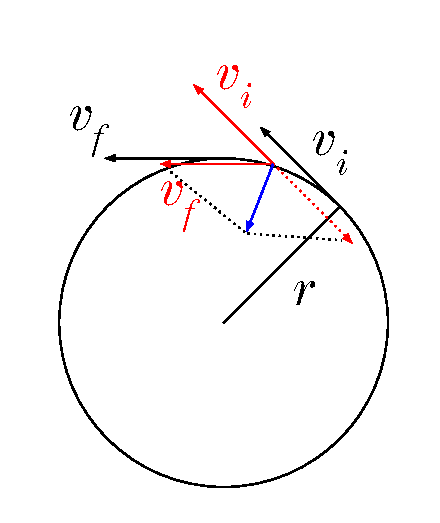
\includegraphics[width = \marginparwidth]{accelerazione_centripeta.pdf}
    \caption{Dimostrazione delle caratteristiche geometriche del vettore accelerazione centripeta.}
    \label{circolare}
\end{marginfigure}
consideriamo una variazione molto piccola nella posizione angolare dell'oggetto,
che parte con una velocità iniziale $\mathbf{v}_i$ e termina con la
velocità finale $\mathbf{v}_f$, uguali in modulo ma diverse in direzione.
Come già detto, possiamo esprimere l'accelerazione come variazione della
velocità tangenziale.

\[ \mathbf{a} = \frac{d\mathbf{v}}{dt} \simeq \frac{\Delta\mathbf{v}}{\Delta t} \]

\noindent Concentriamoci sul termine $\Delta\mathbf{v}$.

\[ \Delta\mathbf{v} = \mathbf{v}_f - \mathbf{v}_i = \mathbf{v}_f + (-\mathbf{v}_i) \]
Geometricamente, i vettori velocità si sommano secondo la ``regola del parallelogramma''
come mostrato nella Figura. Con i dovuti formalismi geometrici, sapendo che il
modulo di $v$ è sempre costante, possiamo dimostrare che l'accelerazione è
effettivamente centripeta e ortogonale alla velocità tangenziale, ovvero il
suo vettore punta sempre verso il centro della circonferenza. Sempre dalla Figura,
possiamo osservare che al crescere di $v$ cresce anche $a$; tenendo poi
presente che la variazione $\Delta \mathbf{v}$, che è un vettore,
viene moltiplicata per la quantità scalare $\frac{1}{\Delta t}$, il vettore
risultante dell'accelerazione cresce in modulo quanto più piccolo diventa
l'intervallo $\Delta t$: ovvero la velocità dell'oggetto è maggiore.
Dimostreremo più
avanti che la relazione precisa tra i moduli di queste grandezze è data da
\[ a = \frac{v^2}{r} = \omega^2 r \]

\section*{Moto armonico}
Supponiamo di osservare un oggetto in moto circolare uniforme, ma invece di
vederlo ``dall'alto'' lo guardiamo con la riconferenza della traiettoria
posta orizzontalmente. Da questo punto di vista, vedremo l'oggetto \textit{oscillare}
a destra e sinistra all'interno di uno spazio la cui larghezza corrisponde al
diametro della circonferenza. Ciò che si vede è un moto particolare, il
\textit{moto armonico semplice}.

Dalla Figura \ref{armonicosemplice} possiamo notare che, fissato il solito
sistema di riferimento $xy$, il moto armonico semplice non è altro che la
proiezione sugli assi di un moto circolare uniforme. Per questo motivo,
possiamo descrivere la posizione dell'oggetto caratterizzato da tale moto:
\begin{marginfigure}
    \centering
    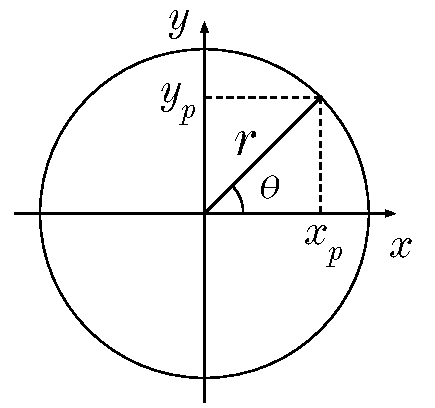
\includegraphics[width = \marginparwidth]{da_circolare_ad_armonico.pdf}
    \caption{Modello di moti armonici semplici a partire da proiezioni
    di un moto circolare uniforme.}
    \label{armonicosemplice}
\end{marginfigure}
\[
    \begin{cases}
        x_p(t) = r\cos\theta = r\cos(\omega t)\\
        y_p(t) = r\sin\theta = r\sin(\omega t)
    \end{cases}
\]
Possiamo quindi notare che il moto circolare è la composizione di due moti
armonici.
Sapendo che la velocità corrisponde alla derivata della funzione che
descrive la posizione:
\[
    \begin{cases}
        v_x(t) = -\omega R \sin(\omega t)\\
        v_y(t) = \omega R \cos(\omega t)
    \end{cases}
\]
Derivando nuovamente, otteniamo l'accelerazione:
\[
    \begin{cases}
        a_x(t) = -\omega^2 R\cos(\omega t)\\
        a_y(t) = -\omega^2 R\sin(\omega t)
    \end{cases}
\]
Esiste anche una dimostrazione geometrica di tali relazioni, che non impiega
esplicitamente i metodi del calcolo infinitesimale. È sufficiente tenere in
considerazione la posizione angolare $\theta$, avere dimestichezza con le
funzioni sinusoidali e ricordare direzione e verso dei vettori velocità
tangenziale e accelerazione centripeta durante un moto circolare uniforme.

\subsubsection*{Relazione tra accelerazione centripeta e velocità}
Siamo ora in grado di mostrare l'origine della relazione $a = \frac{v^2}{r} = \omega^2 r$
tra accelerazione centripeta e velocità (angolare e tangenziale) in un moto
circolare uniforme.

Osserviamo che il sistema che descrive l'accelerazione del moto armonico
contiene i termini $r\cos(\omega t)$ e $r\sin(\omega t)$: le coordinate del
punto in moto circolare uniforme in funzione del tempo. Dunque

\[
    \begin{cases}
        a_x(t) = -\omega^2 r\cos(\omega t)\\
        a_y(t) = -\omega^2 r\sin(\omega t)
    \end{cases}
    \Rightarrow
    \begin{cases}
        a_x(t) = -\omega^2 x(t)\\
        a_y(t) = -\omega^2 y(t)
    \end{cases}
\]
Queste non sono altro che le componenti dell'accelerazione centripeta
solidali al sistema di riferimento di assi $xy$. Sapendo che il modulo
di un vettore corrisponde a $|\mathbf{r}| = r = \sqrt{x_r^2 + y_r^2}$
(con $x_r,y_r$ le componenti del vettore $r$ rispetto ad un sistema di
assi ortogonali $xy$), è immediato mostrare che
\[ |\mathbf{a}| = a = \sqrt{(-\omega^2 x)^2 + (-\omega^2 y)^2} = \sqrt{\omega^4x^2 + \omega^4y^2} = \omega^2 \sqrt{x^2 + y^2} = \omega^2 r \]

Dal precedente sistema, è possibile capire perché il vettore dell'accelerazione
è diretto verso il centro della circonferenza: $x$ ed $y$ sono le componenti
del \textit{vettore posizione} dell'oggetto in movimento; tale vettore
non è altro che una freccia di modulo uguale alla lunghezza del raggio e la
cui punta indica il punto in cui il corpo si trova sulla circonferenza,
dunque questo vettore punta verso l'esterno; ma dato che ogni componente
viene moltiplicata per la quantità negativa $-\omega^2$, il vettore
accelerazione centripeta non può che puntare nel verso opposto, quindi
verso il centro della circonferenza. L'equazione vettoriale è dunque la
seguente:
\[ \mathbf{a} = -\frac{\mathbf{v}^2}{\mathbf{r}} \]

\section*{Moto nel piano}

\subsubsection*{Parabola di un proiettile}
\[
    \begin{cases}
        x = v_{0,x}t\\
        y = v_{0,y}t - \frac{1}{2}t^2
    \end{cases}
\]
Esprimiamo $y$ in funzione di $x$:
\[
    y = \frac{v_{0,y}}{v_{0,x}}x - \frac{1}{2}\frac{g}{v_{0,x}^2}x^2 = Bx - Cx^2
\]
Tangente a questa parabola:
\[
    y' = B - 2Cx
\]

\subsection*{Vettori}
Vettori posizione e spostamento.
\[ \Delta\mathbf{s} = \mathbf{s}_f - \mathbf{s}_i \]

Vettore velocità
\[ \mathbf{v} = \lim_{\Delta t \to 0}\frac{\Delta\mathbf{s}}{\Delta t} = \frac{d\mathbf{s}}{dt} \sim ds\cdot\frac{1}{dt} \]
Per definizione \textit{sempre} tangente alla traiettoria. La traiettoria
è la serie dei punti che si ottiene percorrendo per tratti infinitesimi le
velocità istantanee.

Accelerazione tangente e accelerazione normale.


\subsubsection*{Esercizio}
$|\mathbf{v}_i| = 50\text{ km/h}$, $|\mathbf{v}_f| = 100\text{ km/h}$,
$m = 1800\text{ kg}$, $R = 20\text{ m}$, $\Delta t = 2\text{ s}$. $|\mathbf{F}_n| = ?$ (forza normale),
$|\mathbf{a}_t| = ?$. Assumiamo che l'auto acceleri con costanza tra le
due velocità.

\begin{itemize}
    \item $a_{n,i} = \frac{v_i^2}{R}$, $a_{n,f} = \frac{v_f^2}{R}$
    \item $F_{n,i} = ma_{n,i} \simeq 17100 \text{ N}$, $F_{n,f} = ma_{n,f} \simeq 68400\text{ N}$
    \item $|\mathbf{a}_t| = \textit{cost} = \frac{|\Delta\mathbf{v}|}{\Delta t} \simeq 6,95\text{ m/s}^2$
\end{itemize}

\section*{Recap}
\[ \mathbf{x} = \mathbf{x_0} + \mathbf{v}(t - t_0) \]
Semplificazioni in termini di variazioni, infinità.
\chptr{Dinamica}
\marginpar{\minitoc}

\section{Le leggi della dinamica}

Nella descrizione introduttiva del moto, non è stata analizzata alcuna causa del
fenomeno. Cioè, non ci siamo mai preoccupati di studiare \textit{cosa}
fa muovere un oggetto, ma solo di \textit{come} esso si muove. In
questo capitolo affronteremo lo studio quantitativo di questi agenti
esterni, che si uniscono sotto il termine di \textit{forze}. La dinamica
è il campo che si occupa di queste entità e fonda le proprie radici su
tre principi formulati da Newton.

\subsection{La prima legge}

\begin{tcolorbox}[colback = red!30, colframe = red!30!black, title = {Prima legge della dinamica (legge di inerzia)}]
    Un corpo permane nel suo stato di \textit{quiete} o moto rettilineo uniforme
    finché non intervenga un \textit{agente esterno}.
\end{tcolorbox}

\noindent In altre parole, se nulla ``rompe le scatole'' al corpo, esso permanerà nel suo
stato di moto, naturalmente.

\begin{tcolorbox}[colback = yellow!30, colframe = yellow!30!black, title = {Sistema inerziale}]
    Sistema nel quale vale la prima legge della dinamica.
\end{tcolorbox}

\subsection{La seconda legge}
Quando l'agente esterno agisce sull'oggetto, l'effetto è un cambiamento nello
stato di moto di quell'oggetto. Ovvero, cambia la sua velocità. La variazione
della velocità nel tempo è chiamata \textbf{accelerazione}.

\[ \lim_{\Delta t \to 0} \frac{\Delta v}{\Delta t} = \frac{dv}{dt} = a \]


\begin{tcolorbox}[colback = red!30, colframe = red!30!black, title = {Seconda legge della dinamica}]
Il cambiamento dello stato di moto è proporzionale all'intensità della forza applicata.
    \begin{align}
        F \propto a
    \end{align}
Inoltre, il cambiamento avviene lungo la retta secondo la quale la forza
si applica.
    \begin{align}
        \vecsymb{F} = m \vecsymb{a}
    \end{align}
\end{tcolorbox}

\noindent Gli oggetti hanno inerzia, ovvero capacità di opporsi all'agire dell'agente
esterno. Questa capacità di opporsi è rappresentato da una quantità detta
\textit{massa inerziale}. Essa è la costante di proporzionalità che lega forza applicata
e accelerazione: fissata una accelerazione $a$, più $m$ è grande, tanto più $F$ cresce.
Questo è l'effetto tangibile dell'inerzia.

\subsection*{Analisi dimensionale}
\[ [F] = [ma] = \left[m\cdot\frac{v}{t}\right] = \left[m\cdot\frac{l}{t^2}\right]  \]
\[ 1\text{ kg}\cdot\frac{\text{m}}{\text{s}^2} = \text{udm}\left[M\cdot\frac{L}{T^2}\right] = \text{udm}[F] = 1\text{ N} \]



\subsection{La terza legge}
\begin{tcolorbox}[colback = red!30, colframe = red!30!black, title = {Terza legge della dinamica (legge di azione e reazione)}]
La forza che un corpo $A$ esercita su un corpo $B$ è uguale e opposta alla forza
che

\[ \vecsymb{F}_{A\to B} = -\vecsymb{F}_{B\to A} \]
\end{tcolorbox}




\section{Forze}
Il mondo che ci circonda è costituito da oggetti che esercitano delle azioni gli
uni sugli altri. Tali azioni impresse da agenti esterni su altri agenti sono
generalmente chiamate \textit{forze}, ma possono avere natura differente a seconda
del fenomeno fisico in esame. Ad esempio, le forze possono agire per contatto, come
la spinta delle ruote di un'auto sull'asfalto, o a distanza, come la forza di gravità.
Rimane tuttavia la caratteristica comune del loro \textit{effetto}, ovvero la capacità
di modificare il moto dei corpi in accordo con la seconda legge della dinamica.

Tra le forze più familiari che affronteremo in questo corso ci sono:
la forza elastica; il peso; l'attrito.

\subsection{Forza elastica}

\[ F \propto \Delta x \]

La forza che la molla esercita, essendo in opposizione alla direzione nella
quale la deformazione viene effettuata, corrisponde a:
\[ F_\textit{el} = -k\Delta x \]


\subsection{Peso}
Associamo spesso il peso alla difficoltà nel sollevare un certo oggetto.
Il peso è correlato alla massa in accordo con la seconda legge della
dinamica, ma non si deve assolutamente confondere queste due quantità.
Come vedremo nei prossimi capitoli, il peso deriva dall'interazione
gravitazionale tra corpi dotati di massa.

Sulla Terra, il peso di un oggetto è approssimabile secondo la legge

\begin{align}
    \vecsymb{P} = mg
\end{align}

\noindent dove $g$ corrisponde all'accelerazione di gravità terrestre
in prossimità del terreno. Questa legge vale anche per altri pianeti,
ma a seconda della loro massa il peso di un oggetto può essere differente:
l'attrazione gravitazionale sulla Luna è più debole rispetto alla Terra,
il che rende più leggeri i corpi che si trovano sulla sua superficie.

\subsection{Attrito}
Anche la più liscia delle superfici, se osservata a livello atomico, risulta
scabra. Per far scorrere due superfici l'una sull'altra, occorre superare la
resistenza dovuta agli urti fra i loro minuscoli avvallamenti e sporgenze. Questo
modello grossolano spiega intuitivamente l'origine della forza chiamata
\textit{attrito}. Esso dipende da molti fattori, come il materiale, la finitura
delle superfici, la presenza di lubrificanti, e pertanto non esiste una legge
fisica semplice ed universale che lo descriva. È tuttavia possibile derivare
alcune leggi empiriche in grado di calcolare le forze di attrito.

\subsubsection*{Attrito radente}
L'attrito radente si manifesta durante lo scivolamento tra due superfici (esiste
anche l'attrito volvente, che riguarda corpi estesi che rotolano e ruotano, ma non
è di nostro interesse dato lo studio del punto materiale). La forza di attrito
radente è proporzionale alla forza normale alla superficie ma è indipendente dalla
superficie di contatto fra le superfici ed è espressa dalla relazione
\[ \textbf{F}_A = \mu\mathbf{F}_\perp \]
dove $\mathbf{F}_\perp$ è la forza perpendicolare, o premente, alla superficie,
mentre $\mu$ è un coefficiente di attrito che dipende dai materiali degli oggetti
e altri fattori e spesso è compreso tra 0 e 1.

Le forze di attrito si suddividono a loro volta in attrito \textit{dinamico} e
\textit{statico}.

\subsubsection*{Attrito dinamico}
L'attrito dinamico si oppone allo scorrimento di un corpo su una superficie.

\subsubsection*{Attrito statico}
L'attrito statico si oppone al distacco di un corpo da una superficie. Esso tende
a impedire che un oggetto fermo su una superficie si distacchi da essa, cominciando
a scivolare. L'attrito statico è generalmente maggiore di quello dinamico, perché,
quando le supefici sono in contatto statico, i loro microscopici avvallamenti
(riprendiamo il modello introdotto per spiegare l'origine dell'attrito)
possono aderire maggiormente l'uno all'altro, determinando una maggiore
interazione tra superfici.

\subsubsection*{...}
$\mathbf{F_A} = \mu|\mathbf{N}|\hat{A}$. Grafico, zona statica
forza di attrito statica, regime dinamico forza di attrito dinamica.

Statica
\begin{align}
    \mathbf{F}_{A,S} = -\mathbf{F}_{\text{app}, T}\\
    |\mathbf{F}_{A,S} = |\mathbf{F}_{A,S}^\text{max}| = \mu_s|\mathbf{N}|
\end{align}
Dinamica
\begin{align}
    \mathbf{F}_{A,D} = -\mu_d|\mathbf{N}|\hat{v}
\end{align}



\section{Forze agenti sul moto}
Ci occupiamo brevemente di alcuni problemi comuni di dinamica, nei
quali forze di svariato genere modificano lo stato di moto dei corpi.
Prenderemo come esempio il lancio in verticale con caduta libera e
l'automobile che accelera e frena. Considereremo solo moti in una
dimensione (su una linea retta), ma è possibile applicare gli stessi
ragionamenti alle componenti di moti nel piano e nello spazio.

\subsection{Lancio verticale e caduta libera}

\subsection{Accelerazione e frenata orizzontali}


\section{Statica}
Dopo aver affrontato alcuni problemi di dinamica di corpi \textit{in
moto}, ci occuperemo ora di problemi di dinamica nei quali i corpi
sono \textit{immobili}.


\section{Dinamica dei moti armonici}
Tratteremo il moto armonico introducendo elementi di dinamica newtoniana,
studiando in particolare i cosiddetti \textit{oscillatori armonici}.

\begin{tcolorbox}[colback = yellow!30, colframe = yellow!30!black, title = {Oscillatore armonico}]
    Un oscillatore armonico è un oggetto su cui agisce una forza proporzionale,
    in modulo, allo spostamento dalla posizione di equilibrio e diretta in
    verso opposto rispetto a tale spostamento.
\end{tcolorbox}

\noindent Saranno due gli oscillatori armonici di nostro interesse: l'oscillatore a
molla e il pendolo semplice. Tuttavia, esistono numerosi esempi di oscillatori
armonici in natura, come uno snowboarder che compie evoluzioni in un half-pipe o
un atomo che vibra intorno al suo punto di equilibrio, il bilanciere di un
orologio (con le dovute approssimazioni).



\subsection{Le equazioni del moto armonico}
Riprendiamo le equazioni del moto armonico introdotto nel capitolo precedente.
Il cuore pulsante di tutte le leggi orarie del moto armonico è la funzione
periodica, seno o coseno. La scelta tra queste due dipende dal sistema di
riferimento scelto e dalle condizioni iniziali dell'oscillatore. Nel nostro
caso, scegliamo un oscillatore che parte dalla posizione di equilibrio
(e che come vedremo avrà velocità massima in questo punto), quindi utilizziamo
il seno per descrivere la sua posizione in funzione del tempo:
\[ x(t) = A\sin(\omega t) \]
È necessario fare alcune precisazioni: per \textit{posizione} non intendiamo
solo quella spaziale, ma anche, per esempio, quella angolare; inoltre,
l'equazione precedente non è sufficientemente generale, perché abbiamo
implicitamente supposto che l'istante temporale iniziale sia $t_0 = 0$. Per
questo, la legge oraria generale della posizione di un oscillatore armonico
è $x(t) = A\sin(\omega (t - t_0)) = A\sin(\omega t - \omega t_0)$ (è facile
verificare che effettivamente $x(t_0) = 0$, in accordo con la nostra scelta
del sistema di riferimento). In genere la legge si scrive in questo modo
\begin{align}
    x(t) = A\sin(\omega t + \phi)
\end{align}
Introduciamo alcune terminologie tecniche:
\begin{itemize}
    \item \textbf{Ampiezza} $A$: si tratta del massimo spostamento spaziale
    dell'osillatore a partire dal suo punto di equilibrio, in genere assunto
    come origine del sistema di riferimento adottato per la posizione. Nell'esempio del moto
    circolare, corrisponde al raggio della circonferenza. L'oscillatore si
    muove di fatto tra il massimo $A$ e il minimo $-A$.

    \item \textbf{Pulsazione} $\omega$: è un indice della ``rapidità''
    dell'oscillatore nel compiere i suoi cicli. Approfondiremo meglio
    l'interpretazione della pulsazione nei prossimi paragrafi.
    
    \item \textbf{Fase} $\phi = -\omega t_0$: intuitivamente, lo
    ``sfasamento'' dell'oscillatore. Incontriamo spesso oscillatori sfasati
    quando essi vengono messi in moto in istanti differenti. Per comodità,
    ometteremo spesso la fase, sottointendendo $t_0 = 0$.
\end{itemize}
Con qualche derivata della posizione, otteniamo velocità e accelerazione
dell'oscillatore in fuznione del tempo:
\[ v(t) = \frac{d}{dt}x(t) = \frac{d}{dt}(A\sin(\omega t + \phi)) = A\omega\cos(\omega t + \phi) \]
\[ a(t) = \frac{d}{dt}v(t) = \frac{d}{dt}(A\omega\cos(\omega t + \phi)) = -A\omega^2\sin(\omega t + \phi) \]
Ecco dunque le leggi orarie generali della velocità e dell'accelerazione di
un oscillatore armonico:
\begin{align}
    v(t) &= A\omega\cos(\omega t + \phi)\label{velarmonica}\\
    a(t) &= -A\omega^2\sin(\omega t + \phi)\label{accarmonica}
\end{align}
Concludiamo scrivendo la legge per eccellenza di un moto armonico, ovvero la
\textit{condizione sufficiente}. Sappiamo che l'accelerazione non è altro che
la derivata seconda della posizione rispetto al tempo:
\[ a = \frac{dv}{dt} = \frac{d^2x}{dt^2} \]
Ma dall'Equazione \ref{accarmonica} notiamo che
\[ a = -A\omega^2\sin(\omega t + \phi) = -\omega^2(A\sin(\omega t + \phi)) = -\omega^2x \]
Dunque
\begin{align}
    \frac{d^2x}{dt^2} + \omega^2x = 0
\end{align}
Abbiamo appena definito matematicamente l'oscillatore armonico: cinematicamente,
in un oscillatore l'accelerazione è proporzionale allo spostamento con costante
di proporzionalità negativa.

\subsubsection*{Interpretazione dell'ampiezza}
\subsubsection*{Interpretazione della fase}
\subsubsection{Interpretazione della pulsazione}
In tutte le equazioni dei moti armonici dominano le funzioni goniometriche.
Esse sono periodiche, ovvero esiste una quantità $T$ tale per cui $f(x + T) =
f(x)$ per ogni $x$ appartenente al dominio di $f$. In parole meno fredde,
dopo un certo \textit{periodo} la funzione si ripete, ciclicamente. Per seno
e coseno, il periodo corrisponde a $2\pi$ (infatti, vale per esempio $\sin(x+2\pi) =
\sin(x) \quad \forall x$).

Isoliamo la componente goniometrica delle equazioni armoniche, considerando
per esempio il seno e ignorando la fase $\phi$ (per il coseno il ragionamento
è analogo, mentre per $\phi$ possiamo risolvere il problema mediante trasformazioni).
Supponiamo di avere il periodo $T$, ovvero quel valore per cui la funzione ritorna
uguale a se stessa:
\[ \sin(\omega t) = \sin(\omega(t + T)) = \sin(\omega t + \omega T) \]
Sapendo che il periodo del seno è $2\pi$:
\[ \omega T = 2\pi \quad \therefore \quad \omega = \frac{2\pi}{T} \]
Possiamo dunque comprendere il significato della pulsazione $\omega$:
il suo valore è inversamente proporzionale al periodo $T$, ovvero la
pulsazione cresce al diminuire di $T$, e viceversa. Questo vuol dire
che $\omega$ fornisce un indice della ``rapidità'' con la quale le
oscillazioni di un moto armonico avvengono. Graficamente, $\omega$
comprime verso l'asse dell'ampiezza la funzione goniometrica quando il suo
valore cresce.

\subsection{L'oscillatore a molla}
Consideriamo un carrello di una rotaia a cuscino d'aria di massa $m$ attaccato
ad una molla di costante elastica $k$, indice della durezza della molla. Quando la molla si trova nella
posizione di equilibrio, cioè né estesa né compressa, il carrello rimane
fermo. Poniamo questa posizione come l'origine $x_o = 0$ di un asse delle
posizioni. Se il carrello viene spostato dall'equilibrio e portato a una
distanza $\overline{x}$ da tale posizione, la molla esercita una forza
elastica di \textit{richiamo} che, per la legge di Hooke, corrisponde a
\[ F = -k(x - x_o) = -kx \]
Il segno negativo indica appunto che si tratta di una forza di richiamo,
dunque opposta, nel suo verso, allo spostamento dalla posizione di equilibrio.
Possiamo applicare la seconda legge di newton:
\[ -kx = ma = m\frac{d}{dt}(v) = m\frac{d}{dt}\frac{d}{dt}(x) = m\frac{d^2x}{dt^2} \]
Da cui
\[ \frac{d^2x}{dt^2} + \frac{k}{m}x = 0 \]
È evidente che si tratta di un oscillatore armonico, perché l'accelerazione
è proporzionale allo spostamento, con costante di proporzionalità negativa.
Questa costante è $-\frac{k}{m} = -\omega^2$, da cui possiamo dedurre il
periodo dell'oscillatore a molla:
\begin{align}
    T = 2\pi\sqrt{\frac{m}{k}}\label{periodomolla}
\end{align}

\subsubsection*{Oscillatori verticali}
Anche una massa appesa ad una molla verticale può comportarsi come un
oscillatore armonico. L'unica differenza è la posizione di equilibrio,
nella quale il peso della massa eguaglia la forza di richiamo della
molla:
\[ mg = kx_0 \]
Indipendentemente dal sistema di riferimento utilizzato, l'equazione del
periodo non cambia. La forma delle equazioni armoniche rimane pressoché
invariata, ma è necessario fare attenzione ad eventuali traslazioni spaziali
derivanti dalla scelta del sistema di riferimento.

\subsubsection*{Misurare dinamicamente $k$ di molle per ammortizzatori}
Per misurare la costante elastica di una molla, è immediato tentare un approccio
statico, quindi allungando la molla, registrando la lunghezza di tale allungamento
e la forza di richiamo della molla in seguito alla deformazione. Esiste tuttavia
un metodo ancora più interessante che sfrutta le equazioni armoniche, in particolare
il periodo espresso nell'equazione \ref{periodomolla}.
\[ k = 4\pi^2\frac{m}{T^2} \]
Supponiamo di voler misurare la costante elastica dell'ammortizzatore di un'auto.
Con un po' di ingegno, deduciamo che se affrontiamo un dosso ad alta velocità
l'auto oscillerà verticalmente per qualche istante, per poi assestarsi. Possiamo
dunque stimare il tempo che l'auto impiega per compiere la primissima oscillazione,
che in realtà corrisponderà pressapoco alla metà del periodo di oscillazione.
Infine, conoscendo la massa dell'auto, è possibile utilizzare l'equazione precedente,
ma con una massa divisa per quattro, perché essa viene distribuita sulle quattro
ruote.

%$m = 1500\text{ kg}$ (massa di una ruota per quattro).
%\[ k = m_r\frac{4\pi^2}{T^2} = m\frac{\pi^2}{T^2} \simeq 1500\frac{10}{1\text{ s}}\text{ kg/s$^2$}\]
%$T \simeq 1\text{ s}$.


\subsection{Il pendolo}
Quello del pendolo semplice è un sistema fisico descrivibile mediante
il modello del moto armonico. Un pendolo semplice è formato da una massa
$m$ appesa ad un filo o un'asta (idealmente inestensibili e di massa
trascurabile) con una certa lunghezza $l$. Il punto di equilibrio stabile del pendolo si trova
esattamente al di sotto del punto di sospensione. Di fatto, la posizione
a riposo corrisponde a quella illustrata nel sistema della Figura
\ref{filo}, dove è stato appunto mostrato che la risultante delle
forze agenti sulla massa appesa è nulla.

Supponiamo di spostare la massa dalla sua posizione di equilibrio,
formando un angolo $\theta$ tra il filo e la verticale. Sappiamo che
la massa può oscillare lungo un arco di circonferenza. Fissiamo un
sistema di riferimento solidale alla massa, con un asse coincidente con
la retta passante per il filo e l'altro ad esso perpendicolare, dunque
tangente all'arco. Scomponiamo dunque il peso della massa lungo questi
assi (perpendicolare e tangenziale)  e applichiamo la seconda legge della
dinamica:
\[ ma_t = P_t = -mg\sin\theta \]
\[ ma_n = - P_n + T + F_c = 0 \]
Notare che nella seconda equazione è presente anche la forza centripeta
$F_c$ derivante dal moto circolare, oltre la tensione. Concentriamoci
sull'accelerazione tangenziale nella prima equazione. Ricordando che gli
angoli sono in relazione con la lunghezza degli archi $a$ secondo
l'equazione $a = l\theta$:

\[ a_t = \frac{dv_t}{dt} = \frac{d}{dt} (\omega l) = l \frac{d}{dt}\left(\frac{d\theta}{dt}\right) = l\frac{d^2\theta}{dt^2} \]

\noindent Dunque, riprendendo la primissima equazione riguardo la componente
tangenziale del peso, semplificando la massa:

\[ l\frac{d^2\theta}{dt^2} + g\sin\theta = 0 \]
Per rendere più semplice la trattazione del sistema fisico, supporremo
per ipotesi che $\theta\ll 1$ (in radianti), dunque ciò che calcoleremo
in seguito varrà solamente per piccole oscillazioni del pendolo.
\marginpar{
    \footnotesize
    %\hspace*{-0.5cm}
    \begin{tabular}{c|c|c}
        Prima                      & $\varepsilon\to0$ & Dopo\\
        \hline
        $\sin\varepsilon$          &                   & $\varepsilon$\\
        $\tan\varepsilon$          &                   & $\varepsilon$\\
        $\cos\varepsilon$          &                   & $1 - \frac{\varepsilon^2}{2}$\\
        $e^\varepsilon$            &                   & $1 + \varepsilon$\\
        $(1 + \varepsilon)^\alpha$ &                   & $1 + \alpha\varepsilon$
    \end{tabular}
}
Ricordando le proprietà delle serie di Taylor, possiamo approssimare
il seno nella precedente equazione, dividere per la lunghezza $l$ del
pendolo ottenendo
\[ \frac{d^2\theta}{dt^2} + \frac{g}{l}\theta = 0 \]
Diventa dunque evidente il motivo della semplificazione: abbiamo ottenuto
una relazione nella quale l'accelerazione (angolare) dipende proporzionalmente
dallo spostamento (angolare) con costante di proporzionalità negativa.
In altre parole, si tratta della descrizione di un moto armonico semplice
nella forma $\frac{d^2x}{dt^2} + \omega^2 x = 0$, dalla quale si deduce
che $\omega^2 = \frac{g}{l}$. Ma sapendo che $\omega^2 = (\frac{2\pi}{T})^2$
abbiamo modo di determinare il periodo di oscillazione del pendolo:
\begin{align}
    T = 2\pi\sqrt{\frac{l}{g}}
    \label{periodopendolo}
\end{align}


\subsubsection*{Isocronismo del pendolo}
Come già aveva concluso Galileo nel 1583, il periodo di oscillazione
del pendolo, ristretta ad angoli ridotti a partire dalla posizione
di equilibrio, non dipende dall'ampiezza, come altri moti armonici.
Questo fatto è dimostrato dall'equazione precedentemente ottenuta
(Equazione \ref{periodopendolo}). Ciò che rende un pendolo diverso
dall'altro è la lunghezza del filo e ``il pianeta su cui si trova'',
intendendo l'accelerazione gravitazionale $g$. Mantenendo invariati
questi parametri, possiamo fissare una qualsiasi massa $m$ e caricare
il pendolo a nostro piacere (sempre entro i limiti di angoli ridotti),
ma $T$ non cambierà.

Il fatto che l'oscillazione non dipenda dalla massa fissata trova una
motivazione analoga a quella di una massa in caduta libera, dove
l'accelerazione è sempre la stessa. Masse ridotte si muovono più
facilmente per la loro piccola inerzia, ma tuttavia su di esse agisce
una forza altrettanto ridotta; d'altra parte, masse maggiori sono
sottoposte a forze gravitazionali maggiori, ma sono anche più difficili
da spostare.
Per giustificare intuitivamente l'indipendenza dall'ampiezza, è
sufficiente pensare che una maggiore ``carica'' è compensata da un
tragitto maggiore (l'arco di circonferenza descritto durante
l'oscillazione).
Possiamo dunque concludere che queste compensazioni sono il motivo
delle indipendenze osservabili nell'equazione \ref{periodopendolo}.

\subsubsection*{Analisi approfondita del moto di un pendolo}
Alla luce delle equazioni sul moto armonico semplice, poniamo

\[ \theta = A \sin(\omega t + \phi) \]

\noindent e definiamo la
velocità \textit{angolare} di una massa di un pendolo semplice:
\[ \nu = \frac{d\theta}{dt} = A\omega\cos(\omega t + \phi) \]
Ricordiamo che l'ampiezza $A$ corrisponde all'angolo massimo spazzato
durante l'oscillazione, quindi si tratta di una grandezza adimensionale,
seppur col significato di radianti. Per quanto riguarda l'accelerazione
angolare:
\[ \alpha = \frac{d\nu}{dt} = -A\omega^2\sin(\omega t + \phi) \]
Descriviamo $a$, l'arco di circonferenza descritto durante il moto,
sapendo che la lunghezza del filo è $l$:
\[ a = l\theta = lA\sin(\omega t + \phi) \]
Per quanto riguarda velocità tangenziale e accelerazione tangenziale:
\[ v_t = \frac{da}{dt} = \frac{d}{dt}(l\theta) = l\frac{d\theta}{dt} = l\nu = lA\omega\cos(\omega t + \phi) \]
\[ a_t = \frac{dv}{dt} = -lA\omega^2\sin(\omega t + \phi) \]


\subsubsection*{Tensione del filo di un pendolo semplice in funzione del tempo}
All'inizio di questa sottosezione, abbiamo analizzato le forze in gioco
distinguendo le componenti tangenziali e perpendicolari alla circonferenza
descritta dal pendolo. È ora di analizzare la componente perpendicolare,
la quale permette al pendolo di non distruggersi durante l'oscillazione.
Infatti, la massa è mantenuta nella sua traiettoria per mezzo della tensione
del filo, che si contrappone alla componente perpendicolare del peso della
massa appesa più la forza centripeta derivante dal moto circolare in atto.
La relazione tra i moduli di queste forze è dunque la seguente:
\[T = P_\perp + F_c = mg\cos\theta + ma_c = mg\cos\theta + m\frac{v_t^2}{l} \]
Data la variazione di $\theta$ e di $v_t$ durante l'oscillazione, segue
che la tensione dipende dal tempo. Approssimiamo l'equazione supponendo
$\theta\ll1$, possiamo utilizziare
l'equazione della velocità tangenziale ottenuta precedentemente:
\[ T(t) = mg\cos\theta(t) + mlA^2\omega^2\cos^2(\omega t + \phi) \]
Per via delle approssimazioni, possiamo semplificare anche la funzione coseno
dipendente da $\theta$, rimanendo con il termine $mg(1-\frac{\theta^2}{2})$. Avendo la
descrizione armonica $\theta(t) = A\sin(\omega t + \phi)$ otteniamo la funzione
della tensione di un pendolo per piccole oscillazioni:
\begin{align}
    T(t) = mg\left(1 - \frac{(A\sin(\omega t + \phi))^2}{2}\right) + mlA^2\omega^2\cos^2(\omega t + \phi)
\end{align}



\section{Approfnodimenti}

\subsection{Raggio di curvatura}
L'accelerazione centripeta non esiste solamente nei moti circolari uniformi,
ma, come possiamo ricordare da esperienze quotidiane, qualsiasi variazione
nella traiettoria di un corpo in moto, attraverso una ``sterzata'', permette
di percepire una componente centripeta.
Possiamo dunque estendere la descrizione del moto circolare uniforme a casi
meno eccezionali, come quelli dei moti dalle traiettorie curvilinee. È interessante
come l'equazione dell'accelerazione centripeta permetta di ottenere informazioni
interessantissime su moti come questi, come il \textit{raggio di curvatura}. Si
osservi l'esempio in Figura \ref{curvilinee}.

Tratti di traiettorie come queste possono essere approssimate da archi di
circonferenze con raggi di lunghezze differenti. Durante ognuno di questi brevi
tratti, percorsi sugli archi, l'oggetto in moto è sottoposto ad una certa
accelerazione centripeta. Assumento che tale oggetto abbia una massa, è
possibile misurare l'accelerazione rilevando la forza esercitata sull'oggetto
durante il tratto di curva. Dall'equazione dell'accelerazione centripeta,
vale

\[\frac{F}{m} = \frac{v^2}{r}\]

\noindent Date le nostre supposizioni sulle grandezze conosciute (forza, massa e velocità), l'unico
dato che rimane è il raggio, che in questo caso prende il nome di
\textit{raggio di curvatura}:

\[ r = \frac{v^2m}{F} \]

\begin{marginfigure}
    \centering
    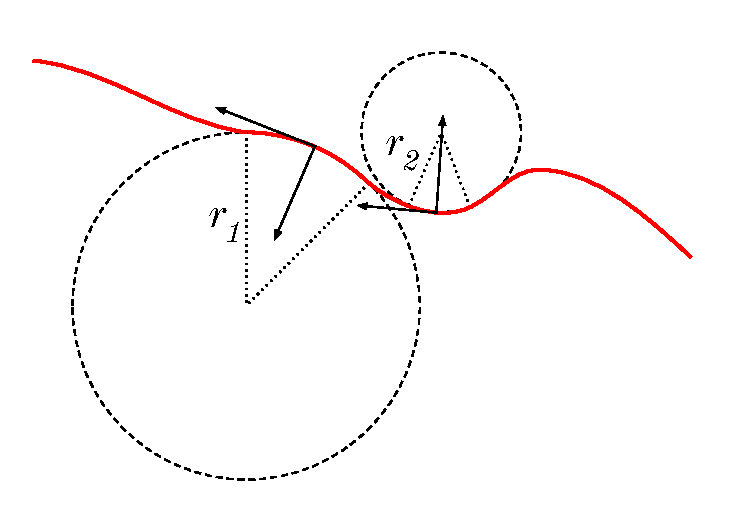
\includegraphics[width = \marginparwidth]{curvilinee.pdf}
    \caption{Una traiettoria curvilinea apporssimata da archi di circonferenze con raggi differenti}
    \label{curvilinee}
\end{marginfigure}































\newpage
\section*{Forza agente sul moto}
Un blocco di massa $m = 10 \text{ kg}$ viaggia ad una velocità $v_i =
2 \text{ m/s}$. Una forza $F = 20 \text{ N}$ agisce sul blocco per
$T = 5 \text{ s}$. Quale velocità raggiungerà il blocco dopo $T$?.
Dopo $T$, la forza cessa di agire e il blocco viaggia a $v_f$ trovata
precedentemente. Includendo lo spazio percorso durante $T$ (e dunque il
tempo $T$), quanto tempo impiega il blocco a coprire $s_w = 2\text{ km}$
di distanza?

\begin{marginfigure}
    \centering
    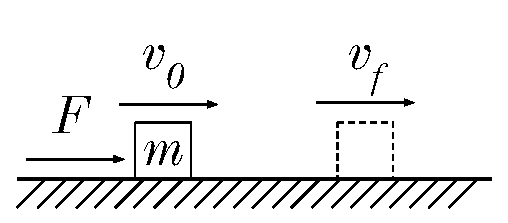
\includegraphics[width = \marginparwidth]{scivola.pdf}
    \caption{Forza agente su una massa in moto}
\end{marginfigure}

Per rispondere al primo quesito, possiamo assumere un moto rettilineo
uniformemente accelerato durante l'intervallo $T$. Sappiamo che \[ a = \frac{F}{m} = \frac{dv}{dt} \]
Da cui possiamo esprimere la velocità in funzione del tempo (la velocità
iniziale la conosciamo già, ma assumiamo un tempo iniziale $t_0 = 0$):
\[ \frac{F}{m}dt = dv \to \int_{t_0}^{t}\frac{F}{m}dp = \int_{v_0}^{v}dw \to \frac{F}{m}\int_{0}^{t}dp = v - v_0 \to \frac{F}{m}t = v - v_0 \]
Dunque
\[ v(t) = v_0 + \frac{F}{m}t \]
Non ci manca che calcolare la velocità in corrispondenza di un $t_f = t_0 + \Delta t = 0 + T = T$:
\[ v(t_f) = v(T) = v_0 + \frac{F}{m}T \]

Nel secondo quesito, possiamo spezzare il problema in due parti: durante
l'azione della forza, la distanza percorsa ($s_a$) deve essere calcolata tenendo
conto del moto uniformemente accelerato, mentre nell'intervallo di tempo
successivo ($T_v$) il moto è semplicemente uniforme. Dalla seguente equazione,
possiamo ricavare $T_v$ ($T$ lo conosciamo già).
\[ s_w = s_a + s_v = s_a + v_fT_v = \int_{0}^{T}(v_0 + at)dp + v_fT_v = v_0T + \frac{1}{2}aT^2 + v_fT_v \]
Il tempo per percorrere $2\text{ km}$ è dunque:
\[ T_{2\text{ km}} = T + \frac{s_w - v_iT - \frac{F}{2m}T^2}{v_f} = T + \frac{s_w - v_iT - \frac{F}{2m}T^2}{v_i + \frac{F}{m}T} \]

\subsection*{Lancio verso l'alto}
Si consideri la situazione mostrata in Figura \ref{lanciobasso}.
Durante la salita, l'oggetto rallenta a causa dell'accelerazione di gravità $g$.
Determiniamo la quota che l'oggetto raggiungerà.

\[ a = \frac{dv}{dt} \to dv = adt \to \int_{v_0}^{v}dw = \int_{t_0}^{t}adp \to v - v_0 = a\int_{t_0}^{t}dp \to v - v_0 = a(t - t_0) \]
Dunque
\[ v(t) = v_0 + a(t - t_0) = v_0 + at \]
Rallentando, si arriverà ad un istante $t_f$ nel quale l'oggetto avrà velocità
nulla:
\begin{marginfigure}
    \centering
    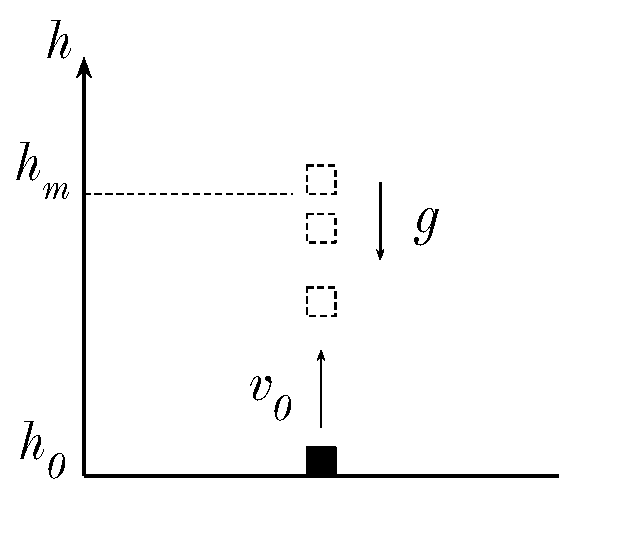
\includegraphics[width = \marginparwidth]{greve.pdf}
    \caption{Lancio di un oggetto verso l'alto}
    \label{lanciobasso}
\end{marginfigure}
\[ v(t_f) = 0 \to v_0 + at_f = 0 \]
Non disponiamo tuttavia del tempo, ma possiamo avvalerci della legge oraria
che descrive la distanza percorsa:
\[ v(t) = \frac{dh}{dt} \to \int_{h_0}^{h}dk = \int_{t_0}^{t}v(t)dp \to h - h_0 = \int_{t_0}^{t}(v_0 + ap)dp \]
\[ h - h_0 = v_0\int_{t_0}^{t}dp + a\int_{t_0}^{t}pdp \to h - h_0 = v_0t + \frac12 at^2 \]
Da cui:
\[ h(t) = h_0 + v_0t + \frac12 at^2 = v_0t + \frac12 at^2 \]
Abbiamo quindi ottenuto la quota in funzione del tempo, che possiamo ricavare
dall'equazione $v_0 + at_f = 0 \to t_f = -\frac{v_0}{a}$.
\[ h(t_f) = v_0t_f + \frac12 at_{f}^2 =  -\frac{v_0^2}{a} + \frac{1}{2}a\frac{v_0^2}{a^2} = -\frac{v_0^2}{a} + \frac{v_0^2}{2a} = -\frac{v_0^2}{2a} \]
Sapendo che $a = -|g|$, la quota massima $h_m$ raggiunta è:
\[ h_m = \frac{v_0^2}{2|g|} \]

%%%%%%%%%%%%%%%%%%%%%%%%%%%%%%%%%%%%%%%%%%%%%%%%%%%%%%%%%%%%%%%%%

\subsection*{Spostamento}
\[ \Delta\mathbf{s} = \mathbf{s}_f - \mathbf{s}_i \]


\section*{Statica}
\[ \sum_{i = 1}^{N}\mathbf{F}_i = m\mathbf{a} \]
La somma nel membro di sinistra è detta \textit{risultante} ($\mathbf{R}$).
In quiete, non c'è accelerazione:
\[ \mathbf{R} = \mathbf{0} \]
Se la velocità è costante, possiamo parlare di problemi di quiete? Yes.

\subsection*{Esercizio}
$\mathbf{P} + \mathbf{T} = \mathbf{0} \Rightarrow -mg + T = 0 \Rightarrow T = mg$.

\begin{marginfigure}
    \centering
    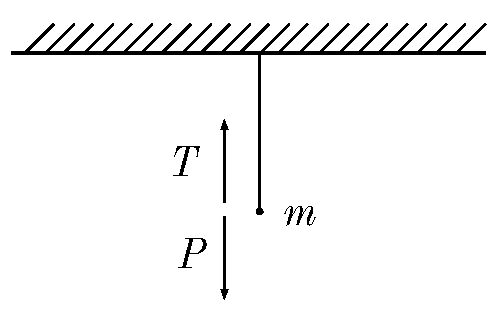
\includegraphics[width = \marginparwidth]{statica.pdf}
    \caption{Massa appesa ad un filo}
    \label{filo}
\end{marginfigure}

\subsection*{Esercizio}
Come quello precedente ma con due corde che tengono $m$, inclinate di
tot gradi fissate al soffitto. Trovare la tensione su ciascun filo.
\chptr{Relatività del Moto}
\marginpar{\minitoc}

\epigraph{\emph{``That view of things would be normal for me if I normally walked on my hands.''}}{\href{https://youtu.be/bJMYoj4hHqU?feature=shared&t=17}{\textcolor{blue}{\textit{Frames of Reference (1960) - Hume, Ivey}}}}

Ciò di cui si tratta in questo capitolo
è stato uno dei temi più controversi nella storia della fisica, quello
che forse ha sconvolto di più convinzioni un tempo ben radicate e
che ha infiammato dibattiti che hanno pure fatto la storia della
letteratura\footnote{\href{https://youtu.be/0kxarmulkiA?feature=shared&t=6180}{\textcolor{blue}{\textit{Marco Paolini - ITIS Galileo}}}.}. E non è tutto qui: Gli ultimi grandi sviluppi della relatività
del moto sono avvenuti poco più di un secolo fa ad opera di Einstein
e molti altri e i cambiamenti da loro apportati hanno condotto a
stravolgimenti ancora più bizzarri. Perché ciò che questo ramo della
fisica rivela è che più osserviamo con attenzione la realtà, più essa non
è come un attimo prima poteva sembrare. Per tale motivo la relatività può
essere allo stesso tempo semplice e complessa, perché offre una visione
del tutto insolita di ciò che ci appare come ``normale''.


\section{Sistemi di riferimento}
``Relativo'' è un termine che ben si sposa con l'espressione ``a qualcosa''.
Quel qualcosa viene definito nelle teorie relativistiche della fisica
\textit{sistema di riferimento}, che intuitivamente rappresenta il punto di
vista dal quale si effettuano delle misurazioni o semplici osservazioni di
fenomeni. Ricordiamo che tra le coordinate di un sistema di riferimento
è presente anche il tempo.

\begin{tcolorbox}[colback = yellow!30, colframe = yellow!30!black, title = {Sistema di riferimento}]
    Un insieme di strumenti geometrico-algebrici, di coordinate solidali con un
    oggetto arbitrario, e di procedure che consentono di individuare la posizione
    di un punto di uno spazio metrico.
\end{tcolorbox}

Una volta fissato il sistema di riferimento, tutte le misurazioni devono
essere coerenti con esso, se si intende adottare quel punto di vista.
Quando diciamo che un'auto viaggia a 110 km/h, stiamo in realtà fornendo
un'informazione incompleta, perché sottintendiamo che tale misurazione
sia stata effettuata rispetto alla strada. Non potremmo dire la stessa
cosa se viaggiassimo su un'altra auto che affianca la prima, con stessa
direzione e verso: Diremmo che
l'auto che prima, vista dalla strada, si muoveva a 110 km/h ora sta viaggiando con velocità
minore rispetto a noi. Il moto di un corpo è sempre relativo a un sistema di riferimento.
Cambiando il sistema, il moto cambia. Vedremo nei prossimi paragrafi
che però non tutti i sistemi di riferimento sono uguali e possono
distinguersi in \textit{inerziali} e \textit{non inerziali}.

Il cambiamento riguarda anche le traiettorie: Se lanciassimo una pallina
verso l'alto mentre viaggiamo sulla carrozza di un treno con velocità
costante, vedremmo la pallina salire e scendere su una linea retta.
Un osservatore esterno, invece vedrebbe la pallina muoversi secondo
una traiettoria parabolica. Vedremo che i moti si compongono
ed è necessario effettuare trasformazioni tra le coordinate dei
sistemi di riferimento.


\section{Principio di relatività galileiana}
In questo corso ci limitiamo a studiare sistemi di riferimento che
descrivono punti materiali che traslano e non ruotano in
alcun modo. Dato che molti oggetti sono in movimento l'uno rispetto
all'altro, vogliamo ora descrivere come essi sono tra loro legati,
ovvero come possiamo ``passare'' da un sistema all'altro, trasformando
le misure effettuate in un sistema in quelle che misureremmo nell'altro.

Supponiamo di avere due sistemi di riferimento, $S$ ed $S'$
centrati rispettivamente in $o$ e $o'$, come mostrati in figura
\ref{sistemi}. Consideriamo poi un punto materiale $P$ qualsiasi
e i vettori posizione che individuano $P$ nei rispettivi sistemi di riferimento:
otteniamo $\vecsymb{r}$, che è la posizione che $S$ misura,
e $\vecsymb{r}'$, misurata invece da $S'$. Ovviamente $S$ e $S'$
devono mettersi d'accordo su quale unità di misura impiegare, per
esempio il metro. Possiamo notare poi che il
sistema $S$ può misurare la posizione del centro $o'$ individuando
il vettore $\vecsymb{oo}'$. Ora è chiaro come questi vettori sono
in relazione:

\begin{align}
    \vecsymb{r} = \vecsymb{r}' + \vecsymb{oo}'\label{relpos}
\end{align}


\begin{marginfigure}
    \centering
    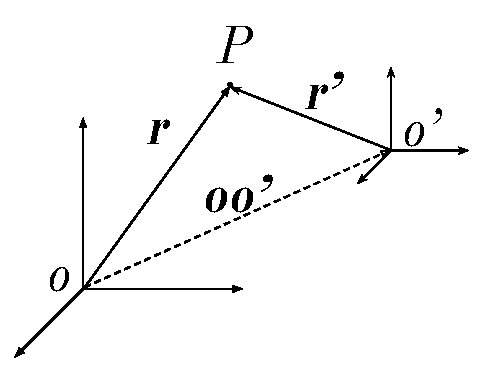
\includegraphics[width = \marginparwidth]{sistemi_relativi.pdf}
    \caption{Relazione tra due sistemi di riferimento che misurano
    la posizione del punto $P$.}
    \label{sistemi}
\end{marginfigure}

\noindent Non abbiamo fatto supposizioni sul moto relativo dei
due sistemi, ma se volessimo estendere l'analisi a velocità e
accelerazione di $P$ rispetto ai due sistemi è sufficiente
applicare alla \ref{relpos} le definizioni di velocità e accelerazione,
come visto in cinematica, derivando l'equazione:

\begin{align}
    \vecsymb{v} = \vecsymb{v}' + \vecsymb{v}_{o'}\\
    \vecsymb{a} = \vecsymb{a}' + \vecsymb{a}_{o'}
\end{align}

\noindent Notiamo che in queste equazioni compaiono $\vecsymb{v}_{o'}$
e $\vecsymb{a}_{o'}$, che corrispondono alla velocità e all'accelerazione
di $S'$ misurate in $S$. Se $\vecsymb{v}_{o'}$ non è nullo, allora
si può concludere che $S'$ si sta muovendo rispetto a $S$. Se $\vecsymb{a}_{o'}$
non è nullo, $S'$ sta accelerando rispetto ad $S$. Ci occuperemo nel seguito del
caso in cui $S$ è inerziale e $\vecsymb{a}_{o'}$ è nullo.

Dal momento che $S$ è inerziale, in esso vale la seconda legge della
dinamica $\vecsymb{F} = m\vecsymb{a}$. Essa avrà la stessa forma anche
in $S'$, che si muove rispetto a $S$ con $\vecsymb{v}_{o'}$ costante?
Ovvero, se $\vecsymb{F}$ è la forza in $S$ e $\vecsymb{F}' = m\vecsymb{a}'$ in $S'$,
varrà $\vecsymb{F} = \vecsymb{F}'$?
Dalle relazioni precedenti, possiamo notare che

\[ \vecsymb{F} = m\vecsymb{a} = m(\vecsymb{a}' + \vecsymb{a}_{o'}) = m\vecsymb{a}' + \frac{d}{dt}\vecsymb{v}_{o'} = m\vecsymb{a}' = \vecsymb{F}' \]

\noindent La seconda legge non è cambiata e possiamo dunque concludere
che $S'$ è un \textit{sistema di riferimento inerziale}.

\begin{tcolorbox}[colback = yellow!30, colframe = yellow!30!black, title = {Principio dei relatività galileiana}]
Le leggi della dinamica newtoniana hanno la stessa forma in tutti i
sistemi di riferimento inerziali.

Con riferimento alle proprietà cinematiche di posizione e velocità di
un punto materiale, il legame tra un sistema di riferimento inerziale,
con origine $o$, e un altro sistema di riferimento inerziale, con
origine $o'$, è descritta dalla seguente trasformazione:

\begin{align}
\begin{cases}
    \vecsymb{r} = \vecsymb{r}' + \vecsymb{oo}'\\
    \vecsymb{v} = \vecsymb{v}' + \vecsymb{v}_{o'}
\end{cases}
\end{align}
\end{tcolorbox}

\noindent In sistemi di riferimento inerziali, la velocità $\vecsymb{v}_{o'}$
prende il nome di \textit{velocità di trascinamento}.


\section{Forze apparenti}


\subsection{L'ascensore}
Per studiare meglio le forze apparenti, consideriamo il classico
esempio dell'ascensore. Quando ci troviamo in ascensore, nel
momento della partenza ci sentiamo più pesanti. Intuitivamente,
ciò accade per via dell'accelerazione della cabina diretta verso
l'alto, che ci preme sotto i piedi. Se invece l'ascensore comincia
a scendere, ci sentiamo invece più leggeri. Notare che ciò accade
solamente quando l'ascensore accelera.

Consideriamo il caso della salita. Trovandoci all'interno dell'ascensore,
immaginiamo di vedere il mondo esterno durante l'accelerazione. Noteremo
che dal nostro punto di vista la cabina rimane ferma, mentre il resto del
mondo scende verso il basso con il modulo della stessa accelerazione
dell'ascensore.


\section{Approfondimenti}
Spesso è facile ingannare la nostra percezione del moto. Le modalità
possono spaziare da tecniche molto semplici a intere teorie, come
quella della relatività di Einstein.

\subsection{Come \textit{Virtual Insanity} è stato girato}

%\section{Approfondimento: RR}
%Questa sezione è interamente dedicata alla relatività ristretta, sviluppata
%nelle sue forme più celebri da Einstein nei primi lustri del Ventesimo secolo.
%Vogliamo dare un assaggio di questa teoria per vari motivi: Si tratta in primo
%luogo di fisica classica (gli strumenti matematici impiegati sono pressoché gli stessi); essa è inoltre un buon esempio di ridefinizione e affinamento
%radicali di teorie precedenti, innanzitutto la relatività galileiana, e convinzioni
%comuni.

%\subsection{I principi della relatività ristretta}
\chptr{Meccanica}
\marginpar{\minitoc}

\section{Energia}
Con la cinematica abbiamo trattato unicamente il moto ``come appare'', slegato
dalle sue cause. Con la dinamica abbiamo invece introdotto quelle cause, ovvero le
forze. In questo capitolo effettueremo un passo in più: Unendo
i concetti definiti fino ad ora, scopriremo una quantità spesso
interpretata come il costo con il quale si pagano cambiamenti e trasformazioni
nell'universo: L'energia. Spiegare cosa sia l'energia valica il confine della
filosofia; la fisica contemporanea si limita a postulare l'esistenza di questa
quantità, misurabile indirettamente da altre quantità, che possiede la peculiare
caratteristica di \textit{conservarsi in sistemi isolati}. In altre parole, se un
sistema non comunica in nessun modo con l'esterno, la quantità di energia di
quel sistema non cambia mai. Essa può al più \textit{trasformarsi} e per questo
motivo non è un qualcosa di tangibile e direttamente osservabile; possiamo solo
vederne le varie forme e manifestazioni. Questo perché l'energia viene sempre
\textit{definita} attraverso altre proprietà invece ben riconoscibili: Distanze,
masse, lo scorrere del tempo. Moltiplicando, dividendo ed effettuando altre
operazioni (che definiremo) di queste quantità su un sistema, scopriremo che
il risutato che si ottiene è sempre lo stesso.

Quella della conservazione è una caratteristica che contraddistingue altre
quantità fisiche, tra le quali vedremo, nel prossimo capitolo, solo la quantità di moto


\section{Lavoro di una forza}
Precedentemente abbiamo introdotto
l'energia come un costo, che può essere convertito e speso per effettuare certi
cambiamenti in natura. Il lavoro di una forza è la forma di energia più familiare,
perché esprime il contributo di una forza allo spostamento di un oggetto, qualcosa
che associamo al moto e dunque ad un'espressione di ``vitalità'': Auto in movimento
mediante il motore,
una persona che cammina per mezzo della muscolatura, un oggetto in caduta libera a
causa del suo peso.

Il lavoro di una forza $\vecsymb{F}$ costante corrisponde al prodotto scalare\footnote{Ricordiamo
che il prodotto scalare $p$ tra due vettori $\vecsymb{a}$ e $\vecsymb{b}$ è un valore scalare
definito da $p = ab\cos\theta_{\vecsymb{ab}}$, con $\theta_\vecsymb{ab}$
l'angolo tra i vettori.}
tra la forza e lo spostamento $\vecsymb{s} = \Delta\vecsymb{r} = \vecsymb{r}_f - \vecsymb{r}_i$,
dove $\vecsymb{r}_i$ e $\vecsymb{r}_f$ sono vettori che descrivono rispettivamente
le posizioni iniziale e finale del punto materiale in moto:

\begin{align}
W \eqdef \vecsymb{F}\cdot\vecsymb{s}\label{workconstforce}
\end{align}

\noindent Il lavoro si misura in Joule (J), dove
\[ 1\text{ J} = 1\text{ Nm} = 1\text{ kg$\frac{\text{m}^2}{\text{s}^2}$} \]

La definizione \ref{workconstforce} presuppone che la forza $\vecsymb{F}$
rimanga sempre constante durante lo spostamento $\vecsymb{r}$. Questo non è
sempre vero nella realtà. Per questo possiamo definire il lavoro infinitesimo
nel seguente modo

\begin{align}
    dW \eqdef \vecsymb{F} \cdot d\vecsymb{s}\label{workvarforce}
\end{align}

\noindent dove supponiamo che per il tratto infinitesimo $d\vecsymb{r}$ agisca
una certa forza costante $\vecsymb{F}$. Se poi definiamo $\vecsymb{F}$ in
funzione dello spostamento, $\vecsymb{F}(\vecsymb{r})$, allora possiamo integrare
su tale funzione per ottenere il lavoro totale tra due coordinate $A,B$.

\begin{align}
    W_{AB} = \int_{A}^{B}\vecsymb{F}\cdot d\vecsymb{s}
\end{align}

\noindent Se si sviscera il prodotto scalare della definizione \ref{workvarforce},
otteniamo

\[ dW = \vecsymb{F}\cdot d\vecsymb{s} = Fds\cos\theta \]

\noindent dove $\theta$ è l'angolo compreso tra i vettori $\vecsymb{F}$
e $\vecsymb{s}$. Notiamo che, per via del prodotto scalare, $dW$ è uno scalare, non un vettore, e
può essere positivo, negativo o nullo. A seconda del caso, il lavoro
viene in genere nominato come segue:

\begin{itemize}
    \item \textit{Lavoro motore:} $dW > 0$
    \item \textit{Lavoro resistente:} $dW < 0$ (la forza si oppone allo spostamento)
    \item \textit{Lavoro nullo:} $dW = 0$ (forza nulla o spostamento nullo o la forza è ortogonale allo spostamento): un
    esempio è la forza centripeta.
\end{itemize}


Esempio cammino sentiero
\[ W_{A\to B} = \sum_{i = A}^{N = B}dW_i \to \int_{A}^{B}dW \text{ per } N\to\infty \]
\[ W_{A\to B} = \int_{A}^{B}\vecsymb{F}\cdot d\vecsymb{r} \]
Notiamo che 
\[ \vecsymb{P}\cdot d\vecsymb{r} = |\vecsymb{P}| (|d\vecsymb{r}|\cos\theta) \]
Dove abbiamo la proiezione dello spostamento sul peso P. Questo significa che
per calcolo del lavoro importa solo la variazione della quota, $dh$.
\[ W_{0\to 2000\text{ m}} = \sum_{0}^{2000}\vecsymb{P}\cdot d\vecsymb{r} = \int_{0}^{2000}mg dh = mgh_{bondone} \]

%\subsubsection*{Versore}
%\[ \hat{v} = \frac{\overrightarrow{v}}{|\overrightarrow{v}|} \]
%\[ W = \int_{i}^{f}\overrightarrow{F}\cdot d\overrightarrow{s} = \int_{0}^{L}(F\hat{f})\cdot(ds\hat{x}) = F(\hat{f}\cdot\hat{x})\int_{0}^{L}ds = F\cos(\theta) L\]
%Quindi
%\[ \cos\theta = \frac{W}{FL} \]







\section{Teorema delle forze vive}
L'ipotesi fondamentale per giungere all'enunciato del teorema
è la seconda legge della dinamica, oltre alla definizione di lavoro.
Supponiamo che $\vecsymb{F}$ sia una forza totale esercitata su
di un corpo di massa $m$. L'azione di $\vecsymb{F}$ produce uno
spostamento, che considereremo infinitesimo in modo da generalizzare
il ragionamento a forze variabili e dipendenti dallo spostamento
stesso. Allora

\[ \vecsymb{F} = m\frac{d\vecsymb{v}}{dt} \]

\noindent Senza giustificare le ragioni matematiche dei prossimi passaggi, ma facendoci
guidare dall'intuizione fisica, eseguiamo il prodotto scalare con $d\vecsymb{s}$
su entrambi i membri
\[ \vecsymb{F}\cdot d\vecsymb{s} = m\frac{d\vecsymb{v}}{dt}\cdot d\vecsymb{s} = m d\vecsymb{v}\cdot\frac{d\vecsymb{s}}{dt} \]
Notiamo che questa operazione ha permesso di ottenere un lavoro al membro di
sinistra, mentre a destra si ottiene il termine $d\vecsymb{s}/dt$, che corrisponderebbe
proprio alla velocità $\vecsymb{v}$. Con ulteriori sviluppi, si raggiunge la
seguente equazione (il simbolo $d$ ha il significato fisico di variazione o
differenza infinitesima).
\[ \vecsymb{F}\cdot d\vecsymb{s} = m\vecsymb{v}\cdot d\vecsymb{v} = m\text{ }d\left[\frac{v^2}{2}\right] \]
Dimostriamo come sviluppare il termine $\vecsymb{v}\cdot d\vecsymb{v} = d\left[\frac{v^2}{2}\right]$.
Ricorriamo alla definizione vettoriale di prodotto scalare\footnote{Il prodotto scalare
di due vettori $\vecsymb{a}$ e $\vecsymb{b}$ è calcolabile anche attraverso la somma
dei prodotti tra i valori delle componenti dei due vettori: $\vecsymb{a}\cdot\vecsymb{b} = a_xb_x + a_yb_y + ...$}
e utilizziamo questo abuso di notazione, ma ragionevole dal punto di vista fisico:
\[ \int x \,dx =  \frac{x^2}{2} + c \Rightarrow \frac{d}{dx}\left[\frac{x^2}{2} + c\right] = x \Rightarrow \int x \,dx = \int d\left[\frac{x^2}{2}\right] \]
Quindi
\[ v_x dv_x + v_y dv_y + v_z dv_z \Rightarrow d\left[\frac{v_x^2}{2}\right] + ... = d\left[\frac{v_x^2 + ...}{2}\right] = d\left[\frac{v^2}{2}\right] \]
Riprendendo l'equazione $\vecsymb{F}\cdot d\vecsymb{s} = m\text{ }d\left[\frac{v^2}{2}\right]$ otteniamo
\[ dW = d\left[\frac12 mv^2\right] \]
Il termine $E_K = \frac{1}{2}mv^2$ viene chiamato \textit{energia cinetica}. Quindi
\[ dW = dE_K \]
Questa equazione può essere tradotta come ``una infinitesima quantità di lavoro
corrisponde ad una variazione infinitesima dell'energia cinetica''. Ora possiamo
enunciare il teorema delle foze vive:
\vspace{8pt}
\begin{tcolorbox}[colback = red!30, colframe = red!30!black, title = {Teorema dell'energia cinetica (o delle forze vive)}]
    Quando una forza (risultante) applicata a un oggetto per un dato tratto di
    traiettoria, compie su di esso un lavoro, il risultato è una variazione del
    modulo della velocità dell'oggetto e quindi una variazione della sua energia
    cinetica. Quindi, il lavoro compiuto su un oggetto è uguale alla variazione
    della sua energia cinetica.
    \begin{align}
        W_{i\to f}^{(R)} = \Delta E_K\label{forzevive}
    \end{align}
\end{tcolorbox}
\vspace{5pt}

\noindent È necessario sottolineare alcune osservazioni:
\begin{enumerate}
    \item Il teorema presuppone che il lavoro sia dovuto all'effetto della risultante delle forze agenti sul corpo.
    \item Il lavoro è rappresentato da una variazione di energia cinetica. Possiamo descrivere dunque lo stato finale
    come \[ E_{K,f} = E_{K,i} + W_{i\to f} \] dunque se il lavoro, quindi l'energia trasferita all'oggetto, è positivo,
    l'energia cinetica aumenta e viceversa.

    \item Il teorema sposta la descrizione del sistema fisico dal piano vettoriale a quello scalare. Ovvero, partendo
    da grandezze vettoriali, abbiamo ottenuto una legge dove compaiono solamente dei numeri. Ciò rende particolarmente agevole
    l'utilizzo del teorema in svariati problemi nei quali l'analisi vettoriale può essere ostica.

    \item Il teorema è molto potente per la sua validità generale, perché non sono state fatte ipotesi sulla natura delle
    forze, se non presupponendo come vera la seconda legge della dinamica $\vecsymb{F} = m\vecsymb{a}$.
    La legge può essere dunque applicata ad un pendolo, ad una palla da bowling,
    a delle molecole microscopiche in movimento.
\end{enumerate}

\section*{Teorema delle forze vive (fato ben)}
Come adesso scopriremo, la definizione del lavoro introduce una
quantità fisica estremamente utile nella trattazione di fenomeni
di natura meccanica. Un risultato molto importante in merito è
il \textit{teorema dell'energia cinetica} (o, come un tempo,
\textit{delle forze vive}, da \textit{vis viva}).

Riprendiamo il secondo principio della dinamica

\[ \vecsymb{F} = m \vecsymb{a} = m \frac{d\vecsymb{v}}{dt} \]



\[ \vecsymb{F} \cdot d\vecsymb{s} = m \frac{d\vecsymb{v}}{dt} \cdot d\vecsymb{s} \]

\noindent dove al memobro di sinistra abbiamo ottenuto il lavoro
infinitesimale corrispondente, $dW$. Osserviamo tuttavia che
al membro di destra vale

\[ m d\vecsymb{v} \cdot \frac{d\vecsymb{s}}{dt} = m d\vecsymb{v} \cdot \vecsymb{v} \]

\noindent per definizione di velocità (istantanea). Osserviamo
dunque ciò che accade passando all'integrazione:

\[ \int_{i}^{f} m \vecsymb{v} \cdot d\vecsymb{v} = m \left[\frac{v^2}{2}\right]_{i}^{f} \]

\noindent Per questo ultimo passaggio, abbiamo fatto ricorso alla
definizione di prodotto scalare e alle proprietà degli integrali:

\[ \int \vecsymb{v} \cdot d\vecsymb{v} = \int v_x dv_x + v_y dv_y + ... = \frac{v_x^2}{2} + \frac{v_y^2}{2} + ... = \frac{v^2}{2} \]

\noindent Abbiamo dunque mostrato che

\[ W_{i \to f} = \frac{1}{2}mv_f^2 - \frac{1}{2}mv_i^2 \]

\noindent ovvero il lavoro totale (derivante cioè dalla risultante
$\vecsymb{F}$ su $m$, come avevamo supposto), dipende solo da
certe quantità che definiscono l'oggetto prima e dopo lo spostamento
nel quale ha agito la forza. La quantità $\frac12mv^2$ corrisponde
dimensionalmente ad una certa energia e viene definita
\textit{energia cinetica}

\[ E_K \stackrel{\text{def}}{=} \frac{1}{2}mv^2 \]

\noindent e rappresenta l'energia che un corpo possiede in
virtù del suo stato di moto, dunque della sua velocità ad un
certo istante.



%\subsubsection*{Applicazione del teorema delle forze vive}
%\textit{Supponiamo di avere un punto di massa $m$ sulla sommità di un piano
%inclinato di alteza $h$ con un angolo $\theta$ rispetto all'orizzontale. Sappiamo
%che la massa parte dalla cima con velocità $v_i$ parallela alla lunghezza del piano
%e diretta verso la discesa. Vogliamo trovare la velocità finale della massa. Si
%esprima il calcolo sia con che senza attrito, considerando nell'ultimo caso un
%coefficiente di attrito dinamico $\mu$.}
%\begin{marginfigure}
%    \centering
%    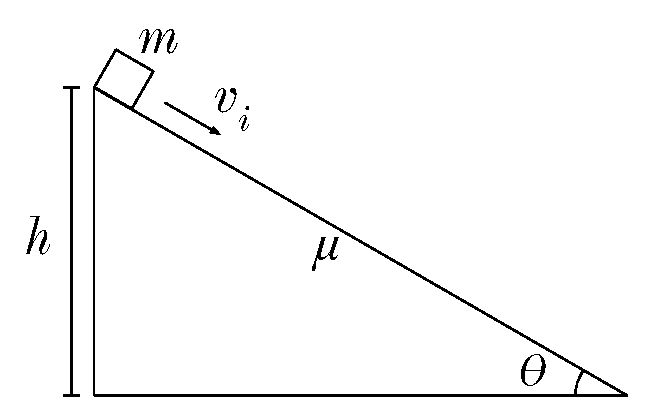
\includegraphics[width = \marginparwidth]{pianoinclinato.pdf}
%    \caption{Un piano inclinato}
%\end{marginfigure}
%\\\\
%Possiamo risolvere il problema utilizzando il teorema delle forze vive.
%\[ W = \Delta E_K \]
%\[ W = \vecsymb{P}\cdot\vecsymb{L} = |\vecsymb{P}||\vecsymb{L}|\cos\left(\frac{\pi}{2} - \theta\right) = |\vecsymb{P}||\vecsymb{L}|\sin\theta = |\vecsymb{P}|h = mgh \]
%\[ \Delta E_K = \frac12mv_f^2 - \frac12mv_i^2 \]
%Quindi
%\[ mgh = \frac12mv_f^2 - \frac12mv_i^2 \]
%\[ v_f = \sqrt{2gh + v_i^2} \]
%
%Con attrito il peso è contrastato. L'attrito compie il suo lavoro per tutta la
%lunghezza del piano fino alla fine della discesa. L'espressione della differenza
%di energia cinetica è tuttavia la stessa.
%\[ W = W_P - W_A = Ph - F_AL = Ph - \mu F_\perp L = mgh - \mu mg\sin\theta L \]
%
%
%\subsubsection*{Problemino}
%Supponiamo di avere un piano inclinato, con attrito e lunghezza $l$, come nel problema precedente.
%La massa viene stavolta lanciata con una velocità iniziale dalla base del piano.
%La massa raggiunge una certa altezza $h$ e poi scivola di nuovo fino in fondo. Si
%vuole determinare la velocità alla quale la massa raggiunge nuovamente la base del
%piano.

\section{Forze conservative}
In fisica, possiamo classificare le forze in \textit{conservative} e \textit{non
conservative}. La distinzione tra di esse sta nel fatto che quando agisce una
forza conservativa, il lavoro compiuto viene immagazzinato in una forma di energia,
\textit{l'energia potenziale}, che è possibile risprigionare. Il lavoro compiuto
da una forza non conservativa, invece, non può essere recuperato in seguito come
energia cinetica, ma viene trasformato in altre forme di energia. Le differenze tra
forze conservative e non conservative emergono se prendiamo in esame il moto di un
oggetto lungo una traiettoria chiusa.

\vspace{8pt}
\begin{tcolorbox}[colback = red!30, colframe = red!30!black, title = {Forza conservativa (condizione I)}]
    Una forza conservativa è una forza che compie un lavoro totale nullo lungo ogni
    percorso chiuso. Se il percorso è $\gamma = A\to A$ (il percorso si chiude su
    se stesso) e $\vecsymb{F}$ è una forza conservativa, allora:
    \begin{align}
        W_{A \to A} = \oint_\gamma \vecsymb{F} \cdot d\vecsymb{s} = 0 \qquad \forall \gamma
    \end{align}
\end{tcolorbox}
\vspace{5pt}

\noindent Da questa prima caratteristica delle forze conservative ne segue nua
seconda. Si considerino i percorsi tra $A$ e $B$ in Figura \ref{percorsi}.
\begin{marginfigure}
    \centering
    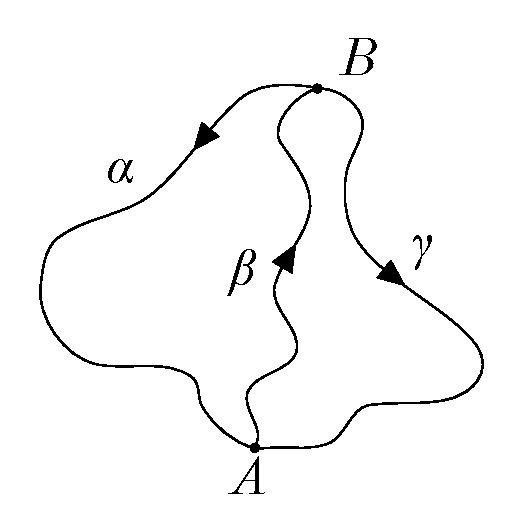
\includegraphics[width = \marginparwidth]{circ.pdf}
    \caption{Percorsi tra due punti in presenza di una forza conservativa}
    \label{percorsi}
\end{marginfigure}
Supponiamo di dover raggiungere il punto $A$ partendo da $B$ e possiamo fare
ciò percorrendo due strade differenti, $\alpha$ e $\gamma$. Disegnamo poi un
terzo percorso, che invece riporta $A$ in $B$.
Per ipotesi vale la condizione I, ovvero sta agendo una forza conservativa
lungo tali percorsi. Dunque, il lavoro compiuto dalla forza nei percorsi chiusi
$\alpha\beta$ e $\beta\gamma$ è nullo:
\begin{align*}
    W_{\alpha\beta} = W_\alpha + W_\beta = 0\\
    W_{\beta\gamma} = W_\beta + W_\gamma = 0
\end{align*}
Ma allora
\[ W_\beta = -W_\alpha = -W_\gamma \quad \therefore \quad W_\alpha = W_\gamma \]
Abbiamo mostrato che il lavoro compiuto dalla forza conservativa dal punto $B$
al punto $A$ è uguale per entrambi i percorsi. In altre parole, il lavoro totale
dipende solo dai punti $A$ e $B$.

Possiamo dimostrare questa proprietà in un altro modo. Consideriamo il percorso
chiuso $\beta\gamma$. Vale per ipotesi
\[ W_{\alpha\beta} = W_\beta + W_\gamma = \int_{A}^{B}\vecsymb{F}\cdot d\vecsymb{s} + \int_{B}^{A}\vecsymb{F}\cdot d\vecsymb{s} = 0 \]
Quindi 
\[ \int_{A}^{B}\vecsymb{F}\cdot d\vecsymb{s} = - \int_{B}^{A}\vecsymb{F}\cdot d\vecsymb{s} = \int_{A}^{B}\vecsymb{F}\cdot d\vecsymb{s} \]

\vspace{8pt}
\begin{tcolorbox}[colback = red!30, colframe = red!30!black, title = {Forza conservativa (condizione II)}]
    Una forza è conservativa se il lavoro totale compiuto da essa durante uno spostamento
    da $A$ a $B$ dipende unicamente da questi punti di partenza e di arrivo, non
    dal percorso seguito tra essi.
    \[ W[\vecsymb{F}]_{A\to B} \text{ indipendente dai percorsi tra A e B} \]
\end{tcolorbox}
\vspace{5pt}

\section{Energia potenziale}
Una forza conservativa può essere caratterizzata da una terza condizione che deriva
dalla seconda.

\vspace{8pt}
\begin{tcolorbox}[colback = red!30, colframe = red!30!black, title = {Forza conservativa (condizione III)}]
    Una forza è conservativa se il lavoro effettuato da essa è esprimibile in
    funzione delle sole ``coordinate'' $A$ e $B$ tramite una primitiva nella forma
    seguente:
    \[ W_{A\to B} = -\left[\mathcal{U}(\vecsymb{x}_B) - \mathcal{U}(\vecsymb{x}_A)\right] = -\Delta\mathcal{U} \]
\end{tcolorbox}
\vspace{5pt}

\noindent Questa condizione esprime la proprietà delle forze conservative di
consentire agli oggetti ad essa sottoposti di immagazzinare una certa quantità
di energia da essa trasferita se l'oggetto passa da $A$ a $B$ e di liberare
quella stessa energia nel tragitto inverso. Immaginiamo di lanciare una palla
nel vuoto. La forza peso, derivante dalla gravità, è conservativa. Mentre la
palla cade, il peso effettua un lavoro su di essa e di fatto la sua energia
cinetica aumenta. Quella energia deve pur provenire da qualche parte. Se osserviamo
questo esperimento ``invertendo il tempo'' (o equivalentemente lanciamo in alto
la palla), osseviamo che la forza peso esegue un lavoro negativo sulla palla,
quindi la sua energia cinetica diminuisce mano a mano. Ma il peso è una forza
conservativa, dunque l'energia da essa sottratta viene comunque conservata
in qualche forma. Questa è l'energia potenziale, che dipende appunto dalla differenza
di quota della palla.

Mostriamo come ricavare la condizione III. Sappiamo che il lavoro di una
forza conservativa è definita da un integrale, che non dipende dal percorso
effettuato tra l'inizio $A$ e la fine $B$. Dunque il lavoro deve in qualche modo
poter essere descritto da una funzione nelle variabili $A$ e $B$.
\[ W_{A \to B} = \int_{A}^{B}\vecsymb{F}\cdot d\vecsymb{s} = f(A,B) \]
Questa funzione sarà una qualche primitiva della funzione integranda, che sarà
quindi composta da dei contributi lineari di $A$ e $B$ dentro qualche funzione
$\mathcal{U}$ (a meno di costanti moltiplicative esterne alla funzione).
Abbiamo quindi le seguenti scelte:
\begin{align*}
    \mathcal{U}(A) + \mathcal{U}(B)\\
    \mathcal{U}(A) - \mathcal{U}(B)
\end{align*}
Ma sapendo che la funzione $f(A,B)$ è una qualche primitiva, ciò significa che
deve valere la proprietà di antisimmetria (invertendo gli estremi di integrazione,
deve cambiare il segno). Questa proprietà vale solo per la seconda funzione:
\[ f(B,A) = \mathcal{U}(B) - \mathcal{U}(A) = - (\mathcal{U}(A) - \mathcal{U}(B)) \]
Definiamo dunque la \textit{differenza di energia potenziale} per forze conservative.
\[ \Delta\mathcal{U}_{A\to B} = \mathcal{U}(B) - \mathcal{U}(A) = -W_{A\to B} \]
Notare che stiamo definendo solo la differenza di energia potenziale, non l'energia
potenziale in sé. Possiamo infatti fissare lo ``zero'' dell'energia potenziale in
modo del tutto arbitrario, in quanto esso non sarà mai utile nel risultato finale
di un problema di meccanica.

\subsection{Energia potenziale gravitazionale}
\subsection{Energia potenziale elastica}

\section{Conservazione dell'energia meccanica}
Ricordiamo il teorema delle forze vive (Equazione \ref{forzevive})

\[ W = E_{K,f} - E_{K,i} \]

\noindent dove $W$ corrisponde al lavoro \textit{totale} delle forze
che agiscono sul corpo tra i momenti $i$ e $f$.
Abbiamo inoltre mostrato che il lavoro dovuto alle forze conservative ($\mathfrak{C}$)
è legato ad una differenza di energia potenziale:

\[ W_\mathfrak{C} = -(\mathcal{U}_f - \mathcal{U}_i) \]

\noindent Per il principio di sovrapposizione, possiamo esprimere il lavoro totale
nel seguente modo, separando l'insieme forze conservative $\mathfrak{C}$ e non conservative $\mathfrak{N}$:

\[ W = W_\mathfrak{C} + W_\mathfrak{N} \]

\noindent Unendo le equazioni finora ottenute,
\begin{align}
    W_\mathfrak{N} = \Delta E_K + \Delta\mathcal{U} = (E_{K,f} + \mathcal{U}_f) - (E_{K,i} + \mathcal{U}_i) = \Delta E\label{nonconserva}
\end{align}

\noindent Abbiamo unito quantità relative a momenti correlati,
cioè abbiamo unito energia cinetica finale con energia potenziale finale
ed energia cinetica iniziale con energia potenziale iniziale.
La somma di queste quantità viene chiamata \textit{energia meccanica}:
\begin{align}
    E \eqdef E_K + \mathcal{U}
\end{align}
Dalla \ref{nonconserva} possiamo notare che, se agiscono forze non conservative,
la variazione di energia meccanica corrisponde al lavoro effettuato dalle
froze non conservative stesse. Per questo, è intuitivo utilizzare l'equazione
nella forma
\[ E_f = E_i + W_\mathfrak{N} \]
perché permette di capire che l'energia meccanica finale del sistema cambierà
da quella iniziale di una certa quantità dovuta all'azione delle forze non
conservative, che possono aggiungere o sottrarre energia meccanica.
In assenza di forze non conservative, allora $W_\mathfrak{N} = 0$.
Segue dunque un importante teorema, ovvero il teorema di conservazione
dell'energia meccanica, che abbiamo appena dimostrato.

\vspace{8pt}
\begin{tcolorbox}[colback = red!30, colframe = red!30!black, title = {Teorema di conservazione dell'energia meccanica}]
    Se su un oggetto il lavoro totale delle forze non conservative è nullo,
    allora la sua energia meccanica si conserva.
    \begin{align}
        \Delta E = 0
    \end{align}
\end{tcolorbox}
\vspace{5pt}


\section{Approfondimenti}

\subsection{Perché ``forze vive''?}
Il lavoro di una forza è ben visibile quando esso agisce su un corpo
in movimento. Prendiamo l'esempio di un razzo che viene lanciato verso
il cielo: La propulsione data dal
propellente spinge il razzo verso l'alto e in termini sempliciotti lo
``aiuta'' a guadagnare velocità durante la salita, perché la forza è
concorde con lo spostamento (entrambi i vettori puntano verso l'alto
perpendicolarmente al terreno) e compie lavoro motore. Quando il razzo raggiunge la sua altezza
massima, in genere comincia a cadere, ma supponiamo che ad un certo
punto esso liberi un paracadute. La resistenza data dal paracadute
determina una forza che si oppone alla caduta del razzo; dunque, in
questo secondo caso, la resitenza dell'aria che gonfia il paracadute
compie un lavoro resistente, che si oppone al moto di caduta e per questo
frena il razzo e ne riduce la velocità.

Agli albori della meccanica ci si sarebbe riferiti all'effetto di queste
forze in gioco come \textit{vis viva}, o forza viva, una quantità o
un'essenza dotata di vita propria,
che trasferendosi da corpo a corpo determinava cambiamenti nello stato
di moto di quegli stessi corpi. Per tale ragione storica, il teorema
porta ancora in sé il termine di forza viva, anche se la fisica
contemporanea propende sempre più verso la denominazione di
\textit{teorema dell'energia cinetica}.
\chptr{Meccanica degli Urti}
\marginpar{\minitoc}

Fino ad ora abbiamo trattato il moto di corpi isolati, ovvero non
perturbati da altri oggetti, ma al massimo influenzati da qualche agente
esterno—le forze. Trattiamo ora gli urti, fenomeni dei quali abbiamo
un'idea intuitiva secondo la quale lo scontro determina un qualche
cambiamento nella velocità e nella traiettoria degli oggetti coinvolti.
Per trattare gli urti è necessario introdurre due nuove grandezze:
quantità di moto e impulso.


\section{Quantità di moto}
Abbiamo sempre espresso la seconda legge come
\[ \vecsymb{F} = m\vecsymb{a} = m\frac{d\vecsymb{v}}{dt} \]
ma questa proposizione afferma che l'effetto dell'agente esterno (la forza
$\vecsymb{F}$) si traduce interamente in una variazione dello stato di
moto del corpo (accelerazione $\vecsymb{a}$). Si suppone quindi che la
massa sia sempre costante, anche se ciò non è sempre vero. Ad esempio,
un razzo pieno di carburante non avrà la stessa massa che aveva in partenza
una volta arrivato in orbita, quindi la forza esercitata dalla propulsione
dei motori si è tradotta non solo in una variazione dello stato di moto,
ma anche in una variaizione della massa. Non tratteremo sistemi complessi
come il razzo, ma ciò fa intuire che la seconda legge della dinamica può
essere generalizzata nella forma seguente
\begin{align}
    \vecsymb{F} = \frac{d}{dt}(m\vecsymb{v}) = \frac{d\vecsymb{p}}{dt}\label{qtamotosecondalegge}
\end{align}
Dove la quantità $\vecsymb{p}$ prende il nome di \textit{quantià di moto},
definita come
\begin{align}
    \vecsymb{p} \eqdef m\vecsymb{v}
\end{align}
Come dice il termine, la quantità di moto descrive il moto dei corpi
sulla base della velocità di una massa più la massa stessa, a differenza
di quanto accade nello studio cinematico del moto, dove solo le variazioni
dello stato di moto contano, slegate da cause (forze) e materia (massa).
La quantità di moto è inoltre una grandezza vettoriale, perché contiene
in sé la velocità, a sua volta grandezza vettoriale.

%L'effetto della quantità di moto si percepisce in molte situazioni quotidiane.
%Nel bowling, possiamo incassare uno strike perché il moto della palla viene
%trasmesso ai birilli, che a loro volta vengono messi in moto e dunque cadono.
%Se immaginiamo di essere su uno skateboard, in grado di muoversi su un piano
%senza attrito, e chiediamo ad un amico di passarci una palla, è sicuro che
%una volta afferrata la palla lo skateboard sul quale ci troviamo comincerà
%a muoversi. Esso sarà inoltre tan


\section{Impulso}
In molte situazioni comuni, le forze agiscono per un tempo brevissimo, come
negli urti. In questi casi è utile introdurre la grandezza dell'impulso.
Supponiamo, ad esempio, che in una partita di baseball il lanciatore faccia
partire la palla a una velocità di 150 km/h. Il battitore ruota il braccio
e colpisce con la mazza la palla, che ritorna verso il lanciatore a 185 km/h.
Nel breve intervallo di tempo durante il quale la palla e la mazza sono in
contatto, dell'ordine del millesimo di secondo, la forza fra esse cresce
rapidamente fino ad un valore massimo molto grande, quindi si annulla quando
la palla si stacca dalla mazza.

Descrivere l'andamento nel tempo della forza che la mazza esercita sulla palla è
difficile. Ciò che possiamo conoscere più facilmente con una strumentazione
adeguata è la \textit{variazione della quantità di moto} (massa e velocità) della
palla a causa del colpo e il tempo $\Delta t$ di contatto tra mazza e palla. Da questi
dati possiamo allora accontentarci di ottenere, usando l'equazione \ref{qtamotosecondalegge} una \textit{forza media}, ovvero
una forza che si è mantenuta costante per tutto l'intervallo di tempo del contatto
mazza-palla.

\[ \left\langle \vecsymb{F}\right\rangle  = \frac{\Delta\vecsymb{p}}{\Delta t} \]

\noindent Riformulando questa equazione per variazioni infinitesime, possiamo
ottenere la variazione di quantità di moto in funzione di $\vecsymb{F}$ e $dt$:

\[ d\vecsymb{p} = \vecsymb{F}dt \]

\noindent Il prodotto $\vecsymb{F}dt$ viene definito \textit{impulso} e non è
altro che una definizione matematica alternativa della variazione della quantità
di moto, utilizzata però più spesso in contesti in cui agiscono forze \textit{impulsive},
cioè forze variabili che agiscono per tempi molto brevi rispetto a quelli
comunemente misurabili nel sistema esaminato.

\begin{align}
    \vecsymb{I} \stackrel{\text{def}}{=} \vecsymb{F}dt\label{impulso}
\end{align}

\noindent L'impulso è particolarmente utile per spiegare il motivo per cui
è più confortevole atterrare su 10 metri di neve dopo una caduta di 100 metri
piuttosto che su una lastra di pietra. Per frenare la nostra caduta, la neve
ci permette di sprofondare al suo interno, quindi essa varia la nostra quantità
di moto in maniera graduale e su un intervallo di tempo prolungato. Al contrario,
la lastra di pietra non si deforma in maniera apprezzabile e l'impatto determina
un impulso molto forte rispetto alla neve, tanto da essere letale.


\section{Il fenomeno dell'urto}

\begin{tcolorbox}[colback = yellow!30, colframe = yellow!30!black, title = {Urto}]
    Un urto è un'interazione tra corpi, nella quale si osservano forze
    denominate \textit{impulsive}, che cioè agiscono per tempi e su distanze
    molto più brevi di quelli \textit{tipici} osservabili all'infuori
    dell'urto.
\end{tcolorbox}
\vspace{5pt}

Cosa si intende per distanze e tempi tipici? Per i lettori che ancora si
ricordano, immaginiamo una puntata di Holly \& Benji: Quando i calciatori
si apprestano a sferrare un calcio, il disegnatore sceglie sempre
di rappresentare l'istante del colpo deformando il pallone. Anche se questa
raffigurazione è evidentemente esagerata, essa ha un fondo di verità e offre una spiegazione
intuitiva di cosa si intende per \textit{distanze tipiche dell'urto}: in un
urto, gli oggetti coinvolti si \textit{deformano}. Queste deformazioni avvengono
su distanze ben minori di quelle, per esempio, della traiettoria del calcio o
della lunghezza del campo. In urti reali, inoltre,
come il calcio alla palla di Holly \& Benji, queste deformazioni sono inevitabili,
nonostante i corpi che collidono sembrino apparentemente i più rigidi su
questo pianeta\footnote{Il suono è prova del fatto che sono avvenute vibrazioni
nei corpi, che dunque si sono deformati.}. Bisogna poi specificare che le
deformazioni sono molto difficili da osservare perché, oltre ad avvenire su
distanze ridotte rispetto a quelle tipiche, anche i tempi nelle quali accadono
sono molto brevi. Il contatto tra piede e pallone è molto ridotto rispetto a
quello che invece è richiesto al calciatore per correre dall'angolo al centro
del campo. Riassumendo questo esempio calcistico, quando osserviamo una
partita siamo di fronte a grandezze \textit{tipiche} (dimensioni del campo da
calcio, velocità dei calciatori e della palla, ecc.); negli urti, invece,
possiamo trascurare le deformazioni e le distanze, perché troppo piccole
rispetto a quelle tipiche, e i tempi, perché gli urti appaiono come eventi
istantanei ai nostri occhi.

L'intenzione della meccanica di questo capitolo, dunque, non è quella di
descrivere ciò che accade \textit{durante} l'urto, ma prevedere, date le
informazioni \textit{precedenti} all'urto, lo stato del sistema
\textit{successivamente} all'urto. Idealmente, l'urto avviene istantaneamente
e i corpi coinvolti sono sempre punti materiali, che dunque non conoscono
deformazioni.

\subsection*{Urti e quantità di moto}
Vogliamo prevedere lo stato del sistema dopo l'urto, in termini di
velocità (vettori) dei corpi coinvolti. Sorprendentemente, gli unici
strumenti che servono per trattare in modo semplice questo problema
sono i tre principi della dinamica, più la definizione di quantità
di moto e l'assunzione del \textit{sistema isolato}, ovvero non
disturbato da forze esterne.

Un classico esempio che unisce nozioni su urti e quantità di moto è il
tavolo da biliardo. Supponiamo di avere due palle, 1 e 2, sul tavolo in moto
rettilineo
uniforme e in rotta di collisione tra loro; ovvero, sappiamo con certezza
che la loro traiettoria si intersecherà e che tale punto verrà raggiunto
da entrambi i corpi nel medesimo istante di tempo. L'esprerienza ci permette
di concludere che, passata la \textit{zona d'urto}, le palle non procederanno
sulle stesse rette dei moti precedenti, ma devieranno.
Dobbiamo fare alcune assunzioni fondamentali. Innanzitutto, supporremo che
nessun altro agente agirà sul sistema appena descritto (aiuterebbe immaginare
due palle che vagano nello spazio profondo, o in altre parole: Nulla deve
disturbare il sistema).
Immaginiamo l'intervallo temporale nel quale le due palle saranno a contatto
tra loro, collidendo: entrambe eserciteranno una forza sull'altra e aiutati
dalla terza legge della dinamica sappiamo che

\[ \vecsymb{F}_{1 \to 2} = -\vecsymb{F}_{2 \to 1} \]

\noindent cioè l'applicazione di una forza su una palla determina una forza identica
in modulo e direzione, ma verso opposto e applicata sull'altra palla.
Sviluppiamo l'equazione sfruttando la definizione di quantità di moto,
ricordando che una forza $x \to y$ determina una variazione dello stato di
moto di $y$.
\[ \frac{d\vecsymb{p}_2}{dt} = -\frac{d\vecsymb{p}_1}{dt} \]
Ricorrendo agli usuali abusi di notazione matematica, ma ragionevoli da
un punto di vista fisico, semplifichiamo l'intervallo di tempo infinitesimale
del differenziale:
\begin{align*}
    &d\vecsymb{p}_2 = -d\vecsymb{p}_1\\
    &d[\vecsymb{p}_1 + \vecsymb{p}_2] = 0\\
    &d\vecsymb{p}_\text{tot} = 0
\end{align*}
Abbiamo mostrato, in anticipo, che per un sistema di due corpi come le palle
da biliardo, assumendo che non agiscano forze esterne, la quantità di moto
totale del sistema si conserva. Come l'energia meccanica, possiamo dunque
concludere che un urto ideale non modifichi la quantità di moto del sistema.
Questa conclusione è ancora incompleta e inesatta perché, come scopriremo
in una prossima sezione, la quantità di moto si conserva \textit{sempre} in
un sistema isolato e non dipende dalla natura dell'urto.

\section{Conservazione}
Come l'energia, nella storia della fisica si è sempre pensasto al moto
come una quantità che potesse essere trasferita da un corpo ad un altro,
fatto ragionevole ben giustificato dall'esperienza: basti pensare al
gioco del biliardo.
Come già dedusse Cartesio, la ``macchina dell'universo'', assimilata ad
un orologio, non può continuare a funzionare senza che una qualche quantità
si conservi. Egli stesso fu tra i primi a proporre il prodotto massa-velocità
come misura di tale quantità: due carri identici che viaggiano a velocità differenti
hanno chiaramente quantità di moto diverse, ma una palla di cannone
racchiude in sé maggior moto rispetto ad un sasso lanciato alla stessa
velocità. Queste quantità sono presenti negli oggetti secondo distribuzioni
differenti e variabili nel tempo, ma nel complesso esse non possono che
sommarsi (vettorialmente!) sempre nella medesima quantità; se l'universo è un
sistema chiuso, e lo si può supporre per definizione, allora la quantità di moto
non può sparire o comparire, ma può trasferirsi tra gli oggetti al suo
interno, trasformarsi.

\subsection{Forze interne ed esterne}
Approfondiamo il concetto di \textit{sistema di punti materiali} e studiamone
uno contentente un certo numero di punti materiali $N$. Immaginiamo che
tra questi punti agiscano forze di varia natura: repulsive elettriche,
attrattive gravitazionali ecc.; inoltre, supponiamo che vengano applicate
altre forze dall'esterno di questo sistema di punti materiali\footnote{Una
immagine esplicativa è il polmone, dove le molecole dell'aria formano i
punti materiali e i muscoli del torace sono gli agenti esterni.}.
Possiamo suddividere le forze in gioco in due insiemi:
\begin{enumerate}
    \item \textbf{Forze interne}: le forze che i punti esercitano gli uni
    sugli altri. Forze che descrivono l'interazione tra i punti.
    \item \textbf{Forze esterne}: le forze che l'ambiente esterno esercita
    sul sistema, l'insieme di punti.
\end{enumerate}
Ogni punto $i$-esimo sarà sottoposto ad una certa forza totale, o risultante, derivante
dalla somma/sovrapposizione di tutte le forze precedentemente descritte
\begin{align*}
    \vecsymb{R}_i = m_i\vecsymb{a}_i\\
    \vecsymb{R}^{(E)}_i + \vecsymb{R}^{(I)}_i = m_i\vecsymb{a}_i
\end{align*}
Definiamo le risultanti delle forze esterne, ed interne agenti sul punto
$i$-esimo:
\begin{align*}
    \vecsymb{R}^{(E)}_i &\eqdef \sum_{k} \vecsymb{F}^{(E)}_{k \to i}\\
    \vecsymb{R}^{(I)}_i &\eqdef \sum_{j} \vecsymb{F}^{(I)}_{j \to i} \qquad j \not = i
\end{align*}
Supponiamo che un punto non eserciti alcuna forza su se stesso (per questo
poniamo $i \not = j$).
La risultante di tutte le forze in gioco sarà
\[ \vecsymb{R} = \sum_{i} \vecsymb{R}_i \]
In tale somma, concentriamoci sulla risultante delle forze interne:
\[ \vecsymb{R}^{(I)} = \sum_{i} \vecsymb{R}^{(I)}_i = \sum_{i} \sum_{j} \vecsymb{F}^{(I)}_{j \to i} \]
In questa somma, supponiamo che non vi siano forze agenti su un corpo
ed esercitate dal corpo stesso, dunque poniamo $\vecsymb{F}^{(I)}_{j \to i} = \overrightarrow{0} \quad \forall j = i$.
Sappiamo che vale la terza legge della dinamica, dunque
$\vecsymb{F}^{(I)}_{j \to i} = -\vecsymb{F}^{(I)}_{i \to j}$. Ma allora
\begin{align}
    \vecsymb{R}^{(I)} = \sum_{i} \sum_{j} \vecsymb{F}^{(I)}_{j \to i} = \overrightarrow{0}\label{interne}
\end{align}
Abbiamo appena dimostrato, grazie all'ipotesi della terza legge,
che, in un sistema di punti materiali, la risultante delle forze interne
è nulla.

\subsection{Centro di massa}
Dall'Equazione \ref{interne} possiamo dedurre che la risultante delle
forze, interne ed esterne, coinvolte in un sistema di punti materiali
è determinata solamente dalle forze esterne.
\[ \vecsymb{R} = \vecsymb{R}^{(E)} = \sum_{i} \vecsymb{R}^{(E)}_i = \sum_i m_i\vecsymb{a}_i \]
Dalla precedente equazione, si può ricavare un'interessante definizione:
\[ \sum_i m_i\vecsymb{a}_i = \sum_i m_i \frac{d^2\vecsymb{x}_i}{dt^2} = \left(\sum_i m_i\right) \frac{d^2}{dt^2}\left[ \frac{\sum_i m_i\vecsymb{x}_i}{\sum_i m_i} \right] \]
Abbiamo ottenuto un termine molto interessante, un artificio matematico
che ha interpretazioni e applicazioni piuttosto importanti: \textit{il
centro di massa}.
\begin{align}
    \vecsymb{x}_\text{CM} \eqdef \frac{\sum_i m_i\vecsymb{x}_i}{\sum_i m_i}
\end{align}
Dalla definizione è banane\footnote{Hai letto bene.} ricavare la velocità e l'accelerazione del
centro di massa. Riprendendo le equazioni precedenti e ponendo $M = \sum_i m_i$,
possiamo concludere che
\[ \vecsymb{R}^{(E)} = M\frac{d^2\vecsymb{x}_\text{CM}}{dt^2} = M\vecsymb{a}_\text{CM} \]

\subsection{La legge di conservazione della quantità di moto}
In un sistema isolato, non si rilevano forze esterne. Allora
\[ \vecsymb{R}^{(E)} = \overrightarrow{0} \quad \therefore \quad M\vecsymb{a}_\text{CM} = 0 \quad \therefore \quad \vecsymb{a}_\text{CM} = 0 \]
ovvero, la velocità del centro di massa è costante, quindi la
quantità di moto del centro di massa è costante e si conserva in
un sistema isolato. Vale dunque la seguente:

\begin{align*}
    \vecsymb{v}_{\text{CM}, i} &= \vecsymb{v}_{\text{CM}, f}\\
    \frac{\sum_j m_j\vecsymb{v}_{j,i}}{M} &= \frac{\sum_j m_j\vecsymb{v}_{j,f}}{M}\\
    \vecsymb{p}_{\text{tot}, i} &= \vecsymb{p}_{\text{tot}, f}
\end{align*}

\noindent Da cui

\begin{align}
    \frac{d}{dt}\vecsymb{p}_\text{tot} = 0
\end{align}
Tale risultato ha conseguenze di portata non trascurabile. Si consideri
infatti il problema esposto nella prossima sottosezione.

\subsubsection*{Punto di collisione}
Due magneti di massa $m$ e $5m$ sono mantenuti ad una distanza fissa tra
di loro. Una volta rimossi i vincoli, i due magneti si attraggono fino a
schiantarsi. Sapendo che il primo magnete si trovava in posizione $x_1 = 0$
mentre il secondo in $x_2 = 8\text{ cm}$, si intende individuare la posizione
della collisione.

Alla luce della legge di conservazione della quantità di moto, sappiamo
che nella situazione iniziale la quantità di moto totale del sistema è
nulla, in quanto i due magneti sono mantenuti fermi.
\[ \vecsymb{p}_i = 0 \]
Il problema non fa alcun cenno all'azione di forze esterne, dunque possiamo
supporre che il sistema sia isolato e che dunque la quantità di moto
iniziale si conserverà anche subito prima dell'urto. Vale allora:
\[ \vecsymb{p}_i = m\vecsymb{v}_{i,\text{tot}} = 0 \Rightarrow \vecsymb{v}_{i,\text{tot}} = 0 \]
Ma sappiamo anche che la velocità totale è rappresentato dal centro di massa
del sistema. Ciò significa che se il centro di massa era ``fermo''
inizialmente, rimarrà tale anche poco prima dell'urto, grazie alla legge
di conservazione della quantità di moto. Basta dunque trovare la posizione
del centro di massa e il gioco è fatto.
\[ x_\text{CM} = \frac{mx_1 + 5mx_2}{m + 5m} = \frac{x_1 + 5x_2}{6} = \frac{5}{6}x_2 \]


\section{Urti elastici}
\begin{tcolorbox}[colback = yellow!30, colframe = yellow!30!black, title = {Urto elastico}]
    In un urto elastico, si conservano la quantità di moto e l'energia cinetica.
\end{tcolorbox}
\vspace{5pt}

\noindent Un sistema contenente un certo numero di corpi può dunque essere descritto come segue:
\begin{align}
    \begin{cases}
        \sum_j m_j\vecsymb{v}_{0,j} = \sum_j m_j\vecsymb{v}_{f,j} \qquad \text{conservazione della quantità di moto}\\
        \sum_j m_j\vecsymb{v}_{0,j}^2 = \sum_j m_j\vecsymb{v}_{f,j}^2 \qquad \text{conservazione dell'energia cinetica}
    \end{cases}
\end{align}
Nella realtà comunemente osservabile, urti pressoché elasti avvengono tra
oggetti che rimbalzano tra loro dopo un urto, anche se in realtà l'energia
cinetica viene inevitabilmente dissipata in altre forme (suono e calore), rendendo
l'urto stesso non del tutto elastico. Sono idealmente elastici urti tra
particelle, a livello molecolare e atomico\footnote{Questa assunzione sarà fondamentale
nella teoria cinetica dei gas}.

\section{Urti anelastici}
\begin{tcolorbox}[colback = yellow!30, colframe = yellow!30!black, title = {Urto anelastico}]
    In un urto anelastico, la quantità di moto del sistema si conserva,
    ma non l'energia cinetica totale.
\end{tcolorbox}
\vspace{5pt}

\noindent Negli urti anelastici, vale sempre la legge di conservazione della quantità
di moto. Tutti gli urti reali sono anelastici e un esempio di urto perfettamente
anelastico è quello di due corpi che rimangono uniti dopo l'urto. Supponiamo di avere due masse che viaggiano ad una certa velocità
e in rotta di collisione tra loro. Dopo l'urto, le due masse rimangono
in contatto. Supponendo che le due masse attaccate formino un unico corpo, Vale:

\[ \vecsymb{p}_{1,i} + \vecsymb{p}_{2,i} = \vecsymb{p}_{3,f} \]

\noindent Dal punto di vista energetico, però, accade qualcosa di strano. Osserviamo
l'energia cinetica:

\[ E_{K,i} = E_{K1, i} + E_{K2, i} = \frac12 m_1\vecsymb{v}_{1,i}^2 + \frac12 m_2\vecsymb{v}_{2,i}^2\]

\noindent Supponiamo di porre gli oggetti nel sistema di riferimento del centro di massa
e di osservare esternamente la situazione (poniamo $\vecsymb{v} = \vecsymb{v}_\text{CM} + \vecsymb{v}_\text{scm}$):

\[ E_{K,i} = \frac12 m_1(\textbf{v}_\text{CM} + \vecsymb{v}_{1,i,\text{scm}})^2 + \frac12 m_2(\textbf{v}_\text{CM} + \vecsymb{v}_{2,i,\text{scm}})^2 = \frac12(m_1 + m_2)\vecsymb{v}_\text{CM}^2 + E'_{K,i} \]

\noindent dove abbiamo isolato i termini nei quali compare la velocità del centro di massa
elevata al quadrato, per poi condensare l'energia rimanente in $E'_{K,i}$,
la cui forma non è per noi rilevante. Se invece calcoliamo l'energia cinetica
finale,
\[ E_{K,f} = \frac12 (m_1 + m_2)\vecsymb{v}_{3,f}^2 = \frac12(m_1 + m_2)\vecsymb{v}_\text{CM}^2 \]
è immediato infatti notare che, data la conservazione della quantità di moto,
il corpo finale comprensivo di entrambe le massse non potrà che muoversi
con velocità identica a quella del centro di massa.
Abbiamo dunque mostrato che in generale l'energia cinetica non si conserva nell'urto.
In particolare, essa diminuisce sempre in situazioni reali.

\begin{align}
    E_{K,f} \leq E_{K,i}
\end{align}

\noindent Il motivo di tale fenomeno può essere spiegato attraverso numerose
interpretazioni, che possono dipendere dal sistema analizzato. In generale,
la perdita di energia cinetica è dovuta al costo per mantenere unite le
masse dopo l'urto, oppure, come accade sempre nella realtà, quell'energia
viene dissipata in calore, deformazioni permanenti dei materiali, suono e
così via.

\section{Aggeggi interessanti}
Sono numerosissimi i sistemi che possono essere resi affascinanti se
analizzati da un punto di vista meccanico. Qui tratteremo solo alcuni
dei più semplici di questi sistemi.

\subsection{Pendolo balistico}
Dedichiamo una sezione ad un dispositivo
molto divertente, che per qualche strano motivo eccita a dismisura la
materia grigia di un qualsiasi fisico: Il pendolo balistico. Scegliamo
questo sistema fisico perché unisce lo studio di quantità di moto ed
energia meccanica, le due principali grandezze conservative affrontate
nel corso.

La figura \ref{ballistico} mostra lo schema essenziale di un pendolo
balistico.
\begin{marginfigure}
    \centering
    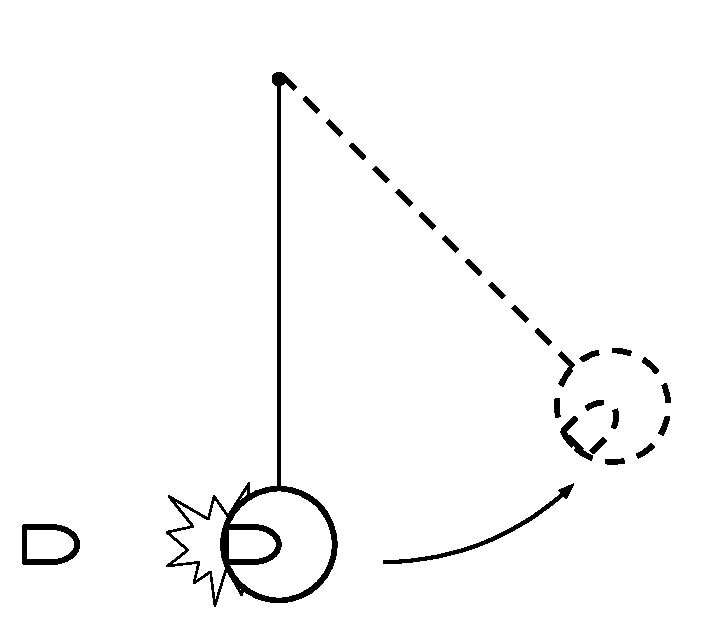
\includegraphics[width = \marginparwidth]{pendolo_balistico.pdf}
    \caption{Il pendolo balistico.}
    \label{ballistico}
\end{marginfigure}
Un pendolo balistico è costituito da due elementi principali: Un
pendolo, costituito da un filo o asta al quale è agganciato un
bersaglio (spesso un sacco di sabbia o un blocco di legno),
e un proiettile. Generalmente, per funzionare bene, ci si aspetta
che la massa del proiettile sia relativamente ridotta rispetto a
quella del bersaglio. Per utilizzare il pendolo balistico, si
spara il proiettile verso il bersaglio fermo, in modo che la traiettoria
del proiettile sia perpendicolare al filo del pendolo. Quando il
proiettile colpisce il bersaglio, esso si conficca al suo interno
e il pendolo comincia ad oscillare per via dell'urto.

Il pendolo balistico è un metodo ingegnoso per misurare in
particolare la velocità del proiettile. Ciò che è sufficiente
conoscere sono le
masse del proiettile ($m$) e del bersaglio ($M$), l'altezza massima di
oscillazione del pendolo ($h$), a partire dalla posizione di equilibrio,
e l'accelerazione di gravità del pianeta
sul quale ci si trova (nel caso della Terra, $g$). Si consideri
l'istante immediatamente precedente all'urto proiettile-bersaglio:
in questo caso, la quantità di moto dell'intero sistema è data dalla
somma della quantità di moto del proiettile e quella del bersaglio
appeso al pendolo, ma sappiamo che quest'ultimo è fermo.

\[ \vecsymb{p}_i = m\vecsymb{v} + M\vec{0} = m\vecsymb{v} \]

\noindent Il proiettile si conficca nel bersaglio, rimanendovi incastrato.
Si tratta dunque di un urto idealmente anelastico. Stavolta il
pendolo comincerà a muoversi con una certa velocità $\vecsymb{V}$
ma la sua massa include quella del proiettile.

\[ \vecsymb{p}_f = (m + M)\vecsymb{V} \]

\noindent La quantità di moto del sistema si conserva e dunque
$\vecsymb{p}_i = \vecsymb{p}_f$, ma supponendo di voler ottenere $\vecsymb{v}$,
serve un'ulteriore
via per trovare l'incognita $\vecsymb{V}$. Per fare questo, ricorriamo alla
meccanica. Immediatamente dopo l'urto, il pendolo comincia
ad elevarsi ad una certa altezza $h$, che possiamo
facilmente misurare, dove il pendolo si fermerà per poi oscillare
ciclicamente. Supponiamo che l'energia cinetica del pendolo sia
massima nel punto di equilibrio e che invece la sua energia potenziale
sia nulla. All'altezza $h$, invece, l'energia cinetica è nulla, perché
il pendolo si ferma per invertire l'oscillazione, mentre l'energia
potenziale è massima. Dal momento che sul sistema solo le forze
conservative compiono lavoro (la forza peso), possiamo applicare il
principio di conservazione dell'energia meccanica.

\[ \Delta E = E_{K_f} + \mathcal{U}_f - (E_{k_i} + \mathcal{U}_i) = (m + M)gh - \frac12(m + M)\vecsymb{V}^2 = 0 \]

\noindent Da cui otteniamo il modulo di $\vecsymb{V}$.

\[ V = \sqrt{2gh} \]

\noindent Passando ai moduli, consapevoli del fatto che i vettori
di $\vecsymb{V}$ e $\vecsymb{v}$ hanno direzione perpendicolare al
filo del pendolo, ricaviamo facilmente il risultato
dall'equazione sulla conservazione della quantità di moto:

\[ v = \frac{m + M}{m}\sqrt{2gh} \]

\noindent Ovviamente questa equazione può essere invertita a piacere
a seconda del dato che si intende individuare, non necessariamente
la velocità del proiettile.


%\subsection{Pendolo di Newton}
%Il famoso pendolo di Newton venne in realtà ideato da Robert Hooke.
%Originariamente, l'artefatto era costituito da tre sferette. In
%tutti i pendoli di Newton, ogni sferetta (di egual massa) è allineata
%e a contatto con le altre, fissate poi mediante fili ad una impalcatura. Sollevando
%e lasciando cadere una delle sferette alle estremità, si mette in moto
%il pendolo, che con fare divertente farà muovere solamente le
%sferette più esterne, mentre quelle interne rimarranno apparentemente
%immobili.


\subsection{Carrelli}
Ammesso che esistano ancora, i fisici si intrattengono nei laboratori
utilizzando anche i carrelli, costituiti da oggetti che scorrono su
binari. È frequente che, per ridurre l'attrito, la rotaia permetta al
carrello di levitare mediante un cuscinetto d'aria. Minimizzare gli
attriti e le dissipazioni è importante, perché ciò consente di giocare
coi carrelli al fine di ottenere degli urti \textit{perfettamente} (in
realtà quasi) elastici e anelastici. Nel seguito illustreremo i più
banali casi di urto perfettamente elastico e urto perfettamente anelastico.

Faremo riferimento alla situazione in figura \ref{carrelli} per
illustrare due scenari tipici.
\begin{marginfigure}
    \centering
    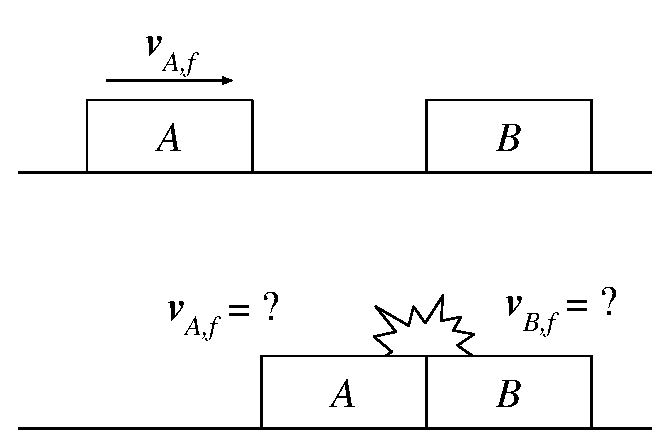
\includegraphics[width = \marginparwidth]{collisione_di_carrelli.pdf}
    \caption{L'esperimento dei due carrelli. $B$ è fermo e lo
    stato di moto futuro dipenderà dalla natura dell'urto (elastico
    o anelastico).}
    \label{carrelli}
\end{marginfigure}

\subsubsection*{Urto perfettamente elastico}
Supponiamo di avere un carrello $A$, di massa $m_A$, che si dirige con velocità $v_A$
verso un carrello fermo $B$ (dunque $v_B = 0$), con massa $m_B$. Il binario è dritto
è dunque il problema si riduce ad una sola dimensione. Supponiamo
che il verso di $\vecsymb{v}_A$ sia positivo. $A$ urta elasticamente
$B$ e il loro stato di moto cambierà in qualche modo a seconda delle
loro masse. Possiamo descrivere il sistema prima e dopo l'urto come
segue:

\[
\begin{cases}
    m_A\vecsymb{v}_A = m_A\vecsymb{v}_{A,f} + m_B\vecsymb{v}_{B,f}\\
    m_A\vecsymb{v}_A^2 = m_A\vecsymb{v}_{A,f}^2 + m_B\vecsymb{v}_{B,f}^2
\end{cases}
\]

\noindent Cerchiamo una forma chiusa con la quale esprimere $\vecsymb{v}_{A,f}$
e $\vecsymb{v}_{B,f}$.

\[
\begin{cases}
    \vecsymb{v}_{B,f} = \frac{m_A}{m_B}(\vecsymb{v}_A - \vecsymb{v}_{A,f})\\
    m_A\vecsymb{v}_A^2 = m_A\vecsymb{v}_{A,f}^2 + m_B \frac{m_A^2}{m_B^2}(\vecsymb{v}_A - \vecsymb{v}_{A,f})^2
\end{cases}
\]

\[
\begin{cases}
    \vecsymb{v}_{B,f} = \frac{m_A}{m_B}(\vecsymb{v}_A - \vecsymb{v}_{A,f})\\
    \vecsymb{v}_A^2 - \vecsymb{v}_{A,f}^2 = \frac{m_A}{m_B}(\vecsymb{v}_A - \vecsymb{v}_{A,f})^2
\end{cases}
\]

\noindent Otteniamo dunque

\begin{align}
\begin{cases}
    \vecsymb{v}_{B,f} = \vecsymb{v}_A\frac{2m_A}{m_A + m_B}\\
    \vecsymb{v}_{A,f} = \vecsymb{v}_A\frac{m_A - m_B}{m_A + m_B}
\end{cases}\label{perfelastico}
\end{align}

\noindent Dalla \ref{perfelastico} possiamo notare che, se $m_A = m_B$,
il carrello $A$ trasferirà tutto il suo moto su $B$ e dunque $A$ si fermerà,
mentre $\vecsymb{v}_{B,f} = \vecsymb{v}_A$. Inoltre, $\vecsymb{v}_{B,f}$
non sarà mai negativo, mentre a seconda della differenza tra $m_A$ e $m_B$
il blocco $A$ potrebbe rimbalzare o proseguire seguendo $B$.

Nella teoria cinetica dei gas impiegheremo la \ref{perfelastico} nei
casi ideali dove $m_A \ll m_B$, o ancor meglio $m_B \to \infty$. Ciò significa
che $A$ rimbalza su $B$ e torna dunque indietro con la stessa velocità
precedente all'urto, ma stavolta con verso opposto. $B$ invece non si
muove.


\subsubsection*{Urto perfettamente anelastico}
Il sistema è lo stesso di prima, ma stavolta l'urto è anelastico.
Supporremo che i carrelli rimangono saldamente uniti tra loro. La
descrizione stavolta riguarda solo la quantità di moto del sistema,
per definizione di urto anelastico:

\[
m_A\vecsymb{v}_A = \vecsymb{v}_f(m_A + m_B)
\]

\noindent e dunque

\[
\vecsymb{v}_f = \vecsymb{v}_A \frac{m_A}{m_A + m_B}
\]

\noindent Qui non è possibile che $\vecsymb{v}_f$ si opponga al
verso di $\vecsymb{v}_A$ (in questo contesto ideale, sarebbe assurdo
se $A$, dopo essersi unito a $B$ fermo, tornasse indietro). $A$
e $B$ rimarrebbero invece immobili dopo l'urto qualora la massa di
$B$ fosse infinitamente più grande di quella di $A$.
\chptr{Gravitazione}
\marginpar{\minitoc}

\section{Forze fondamentali}
Conosciamo bene la seconda legge della dinamica $\vecsymb{F} = m\vecsymb{a}$.
Sappiamo che il termine $\vecsymb{F}$ rappresenta l'azione di un agente esterno,
chiamato forza, che può avere natura diversa a seconda del sistema studiato.
Pertanto, possiamo esprimere
la sua intensità in forme a volte diverse, sia essa il peso, l'attrito, la
forza elastica e così via. Tuttavia tutte queste forze, per quanto sappiamo al
giorno d'oggi, sono riconducibili a quattro interazioni fondamentali che si
manifestano nella materia. Dalla più forte alla più debole, esse
sono:
\begin{itemize}
    \item \textit{Interazione forte}: la più forte tra tutte. Tiene insieme i nuclei
    degli atomi.

    \item \textit{Interazione elettromagnetica}: accoppia le cariche elettriche e
    le correnti.

    \item \textit{Interazione debole}: si manifesta in fenomeni di decadimento nucleare.
    
    \item \textit{Interazione gravitazionale}: la più debole tra tutte.
\end{itemize}
Lo stato attuale della fisica suggerisce che molte di queste forze possano essere
unificate, ovvero esse non sono altro che la manifestazione, in nature differenti,
della stessa forza fondamentale. Molte teorie unificano tra loro le interazioni
elencate, ma qualcosa non permette ancora di mettere a posto alcune di esse,
in particolare la forza di gravità (mannaggia proprio la più scassa-cervello ci
dobbiam sorbire).

Sorprendentemente, è stata la forza più debole ad essere studiata per prima.
La legge fondamentale che descrive come i corpi si attraggono gravitazionalmente tra
loro venne formulata da Newton nel seguente modo:

\begin{marginfigure}
    \begin{center}
        \begin{tikzpicture}
            %corpi 1 e 2
            \filldraw[black] (0,0) circle (2pt) node[below right]{1};
            \filldraw[black] (3.5,3.5) circle (2pt) node[below right]{2};
            
            %vettore distanza
            \draw (1.7,1.7) node[below right]{$\vecsymb{r}_{1,2}$};
            \draw[->] (0.0,0.0) -- (3.45,3.45);

            %vettore forza gravitazionale (UNA SOLA!!!)
            \draw[->] (3.3,3.7) -- (1.5,1.9);
            \draw (2.7,3.5) node[below left]{$\vecsymb{F}_{1,2}$};
        \end{tikzpicture}
    \end{center}
    \caption{Illustrazione dell'applicazione della legge di Newton.
    Anche se non viene mostrata, il corpo 2 esercita la stessa
    forza, ma opposta in verso, sul corpo 1, in accordo con la
    terza legge della dinamica.}
    \label{gravitescionalfors}
\end{marginfigure}

\begin{tcolorbox}[colback = yellow!30, colframe = yellow!30!black, title = {Legge di gravitazione universale}]
    \begin{align}
        \vecsymb{F}_{\text{G}, 1\to 2} = -G\frac{m_{\text{G},1}m_{\text{G},2}}{r^2_{1,2}}\hat{r}_{1,2}\label{gravity}
    \end{align}    
\end{tcolorbox}

\noindent Che esprime il vettore della forza gravitazionale che un corpo 1 esercita su un
altro corpo 2. Come mostrato in figura \ref{gravitescionalfors}, il vettore giace sulla congiungente tra i due corpi (considerati come
punti materiali), separati da una distanza $r_{1,2}$ e dotati di una certa
\textit{massa gravitazionale} $m_G$. Il segno negativo, accompagnato dalla
\textit{costante di gravitazione universale}, indica che la forza gravitazionale è
sempre attrattiva.

\section{Il principio di equivalenza}
Soffermiamoci a chiarire alcuni concetti. Innanzitutto, vogliamo esprimere la legge
\ref{gravity} in maniera più generica.

\begin{align}
    \vecsymb{F} = c\frac{p_1p_2}{r^2}\hat{r} \label{template}
\end{align}

\noindent Sorprendentemente, questa forma verrà proposta da Coulomb per esprimere
l'interazione tra due cariche elettriche, secondo la legge (in moduli)

\[ F_E = k\frac{|q_1||q_2|}{r^2} \]

\noindent Diventa naturale pensare che l'equazione \ref{template} possa rappresentare una
sorta di ``template'' con il quale esprimere quantitativamente l'interazione tra due
oggetti dotati di una certa qualità o proprietà intrinseca $p$, che consente agli oggetti in
questione di partecipare nell'interazione. Nel caso delle cariche elettriche,
essa sarà, per l'appunto, una carica elettrica. Per quanto riguarda la gravità,
questa qualità è la massa gravitazionale. Ci si può chiedere se stiamo parlando
della stessa massa della seconda legge di Newton. In realtà, esse sono ben diverse:
\begin{itemize}
    \item La massa inerziale $m_I$ esprime la capacità di un corpo di opporsi all'azione
    di agenti esterni e, di conseguenza, al cambiamento del proprio stato di moto.
    In breve, essa misura l'inerzia del corpo.

    \item La massa gravitazionale $m_G$ esprime la capacità di un corpo di partecipare,
    contribuire ed essere soggetto all'interazione gravitazionale in presenza di
    un altro corpo dotato di massa gravitazionale.
\end{itemize}
Seppur sottile, la natura di queste quantità è
comunque diversa (un oggetto ``massivo'' è difficile da spostare; un oggetto ``massiccio''
interagisce maggiormente con un altro oggetto). La parola ``carica'' sarebbe più intuitiva per spiegare la differenza
e viene infatti utilizzata per le interazioni elettriche: più carico di una certa
proprietà dell'interazione, più intensa l'interazione stessa. Nella pratica ci
riferiamo sempre alla stessa massa (i kilogrammi), ma nulla impedisce di pensare che le masse di
uno stesso corpo siano effettivamente quantità distinte.

Consideriamo un corpo in prossimità della superficie terrestre. Possiamo approssimare
la Terra ad una sfera uniforme e supporre che la forza gravitazionale corpo-Terra
giaccia sulla congiungente tra il centro del pianeta e il corpo (puntiforme). Il
corpo si trova ad una certa altezza $h$ e conosciamo inoltre il raggio della Terra
$R_T$. Il corpò sarà soggetto alla forza gravitazionale della Terra; uniamo le
equazioni di Newton (consideriamo i moduli):
\[ F = m_\text{I,C}a \qquad F = G\frac{m_\text{G,C}M_\text{G,T}}{(R_{T} + h)^2} \]
Supponiamo che $R_T \gg h$. Dunque la distanza Terra-corpo può essere approssimata:
\[ r_\text{T,C} = R_T + h = R_T\left(1 + \frac{h}{R_T}\right) \]
\[ r_\text{T,C}^2 \simeq R_T^2\left( 1 + 2\frac{h}{R_T} \right) \]
\[ \frac{1}{r_\text{T,C}^2} \simeq \frac{1}{R_T^2}\left( 1 - 2\frac{h}{R_T} \right) \]

\noindent Da cui concludiamo che possiamo trascurare $h$. Dunque, sapendo che
$a = g$,

\[ m_\text{I,C}g = G\frac{m_\text{G,C}M_\text{G,T}}{R_{T}^2} \]

\noindent Isoliamo $g$

\[ g = \frac{m_\text{G,C}}{m_\text{I,C}}G\frac{M_\text{G,T}}{R_{T}^2} \]

\noindent Se assumessimo che le masse inerziale e gravitazionale di uno stesso corpo
sono diverse, l'accelerazione $g$ non sarebbe la stessa per tutti gli oggetti. Tuttavia,
non è ancora stata trovata evidenza della differenza quantitativa (quantomeno apprezzabile,
perché si tratta pur sempre di misure sperimentali) tra le due proprietà. L'osservazione galileiana stessa
sulla caduta libera, ovvero che tutti i corpi cadono con la stessa accelerazione,
indica che

\begin{align}
    m_I = m_G\label{equivalence}
\end{align}

\noindent che rappresenta il principio di equivalenza tra massa inerziale e massa
gravitazionale. Possiamo affermare ciò perché,
fisttata la massa della Terra e il suo raggio,
il rapporto $m_I/m_G$ deve essere costante, anzi uguale a 1,
affinché $g$ sia uguale per tutti i corpi di massa distinta.

\section{Approfondimenti}
Forse il campo della fisica più affascinante è
l'astrofisica. Citiamo solo alcuni approfondimenti infinitesimi rispetto
all'immensità della fisica astronomica\footnote{Così ampia per via della
sua storia millenaria, al contrario della meccanica descritta in queste
pagine}.

\subsection{Energia potenziale gravitazionale}
Si usa spesso calcolare l'energia potenziale di un oggetto vicino alla superficie
terrestre, ad un'altitudine $h$, con la seguente legge:

\[ mgh \]

\noindent Tuttavia sappiamo che $g$ non è costante al variare della quota e su grandi
distanze questa legge non è più una buona approssimazione. Calcoliamo dunque la differenza
di energia potenziale tra la superficie terrestre e una certa quota $h$ da essa alla luce
della legge di Newton.

\[ \Delta\mathcal{U} = -W = -\int_{R}^{R + h}-G\frac{mM}{s^2}\,ds = GmM\int_{R}^{R+h}\frac{ds}{s^2} = GmM\left[ -\frac{1}{s} \right]_{R}^{R+h} =  \]
\[ = -GmM\left( \frac{1}{R + h} - \frac{1}{R} \right) \]

\noindent Notiamo che $\Delta\mathcal{U} > 0$, dunque allontanando un oggetto di massa
$m$ dalla superficie terrestre, esso guadagna una certa energia potenziale. Più in generale,
se poniamo un punto di riferimento $X$ arbitrario dal quale calcolare la (differenza di)
energia potenziale verso un punto $P$, otteniamo la seguente espressione:

\[ \mathcal{U}(P) = -GmM\left(\frac{1}{r_P} - \frac{1}{r_X}\right) \]

\noindent Per convenienza è utile porre $r_X = +\infty$, ovvero ad una distanza infinita da
$M$, ottenendo dunque

\[ \mathcal{U} = -\frac{GmM}{r} \]

\noindent L'energia meccanica di un corpo è dunque

\[ E = E_K + \mathcal{U} = \frac{1}{2}mv^2 -\frac{GmM}{r} \]

\noindent Ovviamente supponiamo che tutte queste leggi valgano per punti materiali.
In un caso reale, per esempio per il calcolo dell'energia potenziale gravitazionale
in prossimità della Terra, quando si sprofonda nel corpo che genera il campo
gravitazionale, l'estensione di tale corpo modifica l'andamento dell'energia potenziale.

\subsection{Eratostene e Cavendish}
Per giungere alla conclusione mostrata nell'equazione \ref{equivalence},
sono necessari due dati molto importanti: Il raggio della Terra e la
costante $G$. Il primo fu misurato già ai tempi di Eratostene. Il secondo
rimase incognito per quasi 100 anni dopo la formulazione della legge
\ref{gravity} da parte di Newton.

Nel 1798 il fisico inglese Henry Cavendish compì un esperimento con
strumentazioni abbastanza sensibili da poter stimare il valore di $G$,
un dato estremamente piccolo (ordine $10^{-11}$!). Nel suo esperimento,
Cavendish utilizzò una bilancia di torsione. Due masse $m$ sono fissate
a un'asta appesa ad un filo (la massa dell'asta è trascurabile).
Accando alle due masse sospese sono poste due grandi masse $M > m$ ferme.
Ciascuna massa $m$ viene attratta, a causa della forza di gravità,
verso la massa $M$ vicina, quindi l'asta che sostiene le masse sospese
ruota e torce il filo. È possibile misurare l'angolo di torsione del
filo riflettendo un raggio di luce su una superficie riflettente
solidale con il filo. Se è nota la forza necessaria per torcere il
filo di un dato angolo (questo è possibile se il filo è stato tarato
con esperimenti precedenti), la misura dell'angolo di torsione fornisce
la maisura dell'intensità della forza di gravità. Conoscendo le masse
$m$ e $M$ e la distanza tra i loro centri, possiamo usare la legge
di Newton per ricavare $G$.
Cavendish ottenne un valore $G = 6.754 \cdot 10^{-11} \text{ Nm}^2/\text{kg}^2$,
in accordo con il valore oggi accettato di $6.67 \cdot 10^{-11} \text{ Nm}^2/\text{kg}^2$.

Avendo a disposizione il valore di $G$, fu quindi possibile determinare
anche la massa della Terra $M_T$:

\[ M_T = \frac{gR_T^2}{G} \]

\subsection{Gravitazione universale}
Secondo la legge di Newton, tutti gli oggetti nell'universo si attraggono l'un l'altro
attraverso l'interazione gravitazionale. è in questo senso che la legge viene detta
universale.

%\subsubsection{Modelli astronomici}

\subsubsection{La terza legge di Keplero}
Ovviamente la legge di Newton ha grande importanza in campo astronomico (anche
se espressa in forme assai più complesse) ed è stata la conferma di una legge scoperta
sperimentalmente tempo addietro da Keplero, appunto la \textit{terza legge di Keplero}:

\[ T \propto r^\frac{3}{2} \]

\noindent Secondo tale legge, il periodo $T$ di rivoluzione di un pianeta attorno al Sole
è proporzionale alla distanza media $r$ del pianeta dal Sole elevata a $3/2$. Dunque esiste
una costante $k$ tale che $T = kr^\frac{3}{2}$. In realtà
questa legge vale per tutti i sistemi astronomici (solari e non) simili al nostro, ma
gli studi di Keplero si basavano sugli attenti dati raccolti dal maestro Tycho Brahe
sui moti orbitali dei corpi celesti appartenenti al sistema solare.

Per dimostrare la terza legge per via teorica, è necessario supporre che il pianeta
in rivoluzione intorno al Sole viaggia secondo un moto circolare uniforme\footnote{Anche se in realtà
l'orbita è ellittica, la distanza media tra pianeta e Sole è la stessa durante una rivoluzione e dunque il
moto è approssimabile a quello circolare.}, del quale conosciamo bene le relazioni che legano periodo, velocità
angolare, velocità tangenziale e accelerazione centripeta: $T = 2\pi/\omega$, $v = \omega r$ e
$a_c = v^2/r$.
Sapendo poi che la forza di gravità tra un pianeta e il Sole è proprio la forza
centripeta del moto orbitale, possiamo effettuare i seguenti calcoli unendo tutte
le leggi scoperte fino ad ora:

\[ T = \frac{2\pi}{\omega} = \frac{2\pi}{v}r = \frac{2\pi}{\sqrt{a_c r}}r = \frac{2\pi}{\sqrt{\frac{GM}{r}}}r = \left(\frac{2\pi}{\sqrt{GM}}\right)r^\frac{3}{2} \]

\noindent Non solo abbiamo dimostrato la terza legge, ma abbiamo pure individuato la
costante di proporizonalità $k$.

\subsubsection*{Sistemi binari}
Dedichiamo questa sezione ad un problema di gravitazione piuttosto complesso,
ma altrettanto interessante, presente peraltro in natura nonostante il classico
modello copernicano al quale siamo abituati.

In sistemi non simili a quello solare vale ancora la legge di Newton. Consideriamo
per esempio un sistema di stelle binarie, ovvero stelle con una differenza di massa
non trascurabile rispetto alla distanza del centro di massa del sistema dal centro
di massa di una delle due stelle. In tale caso, le stelle orbiteranno attorno al
loro centro di massa, situato in qualche punto dello spazio intermedio sulla loro
congiungente. Anche nel sistema solare la Terra e il Sole ruotano attorno al centro
di massa totale, che tuttavia si trova ben al di sotto della superficie del Sole,
il che permette di ridurre la trattazione del problema ad una rivoluzione della
Terra attorno al Sole.
\chptr{Termodimaica - Parte I}
\marginpar{\minitoc}

\section{Introduzione}
In questo capitolo il ruolo dell'energia diventa ancora più
importante. In precedenza abbiamo dimostrato che la differenza di
energia meccanica di un sistema corrisponde al lavoro totale delle
forze non conservative che agiscono sul sistema, quindi $W^\text{NC} = \Delta E$.
In altri termini, l'energia che un sistema possiede viene persa o
acquistata nel caso in cui vi siano forze non conservative che
compiono lavoro su di esso. Ma quindi l'unico modo di ``parlare'',
trasferire energia, ad un sistema dell'universo è quello di compiere
lavoro? In realtà no, come mostreremo parlando di \textit{calore},
un'altra forma di energia \textit{in movimento} come il lavoro, ma
in un certo senso più disordinata.

Ci occuperemo inoltre di sistemi fisici contenenti un numero di
costituenti dell'ordine del numero di Avogadro

\[ N_A = 6 \cdot 10^{23} \]

\noindent Il sistema di questo tipo che più ci interessa è quello
dei gas. Supporremo che i gas sono costituiti da particelle
infinitesime che devono seguire certi comportamenti ideali. Ma
trattandosi di punti materiali, non possiamo studiare questi
sistemi in termini meccanici, secondo la dinamica newtoniana,
come abbiamo sempre fatto? Se seguissimo questa strada, potremmo
non vivere abbastanza per vedere i risultati: Dovremmo prima di
tutto osservare e misurare le caratteristiche cinematiche e
meccaniche di ogni singola particella, quanto meno ad un preciso istante di
tempo (dovremmo dunque misurare tutte le particelle pressoché
contemporaneamente), stilare poi un sistema di equazioni che
descriva le quantità di moto, le energie in gioco ed eventualmente
altre informazioni per analizzare gli urti e prevedere lo stato
futuro del sistema. Due vie alternative sono possibili: La prima è
quella di introdurre nuove grandezze che misurino lo stato globale
del sistema, rinunciando ad elencarne minuziosamente i dettagli come
abbiamo descritto sopra; la seconda, una sorta di compromesso,
è di ricorrere alla statistica. Noi tratteremo qui la prima modalità
per ragioni storiche e semplicità (la seconda, chiamata \textit{meccanica statistica},
è una delle ultime evoluzioni della termodinamica, assai più
complessa della formulazione classica).

In effetti, la ricerca delle relazioni tra le varie proprietà
dei materiali, senza conoscere la loro struttura interna, è l'oggetto
di studio della termodinamica\footnote{Feynman, 44-1}. In realtà cercheremo una spiegazione di certi fenomeni
analizzando ciò che accade nel microscopico, come mostreremo con la
teoria cinetica, ma ciò che soprenderà di più sarà il fatto che effetti
come pressione e variazioni di temperatura sono pressoché indipendenti
dai dettagli interni delle particelle del materiale come le loro singole
collisioni.

\subsection{Sistemi termodinamici}
Le nostre trattazioni avranno per oggetto i \textit{sistemi termodinamici}, per
definizione immersi in un \textit{ambiente esterno}. Ambiente esterno e il suo
contenuto costituiscono l'\textit{universo}, un sistema che per definizione non
è contenuto in un altro ambiente esterno.
Altro oggetto di nostro interesse per lo studio di questi sistemi sono le
\textit{trasformazioni termodinamiche}, ovvero processi nei quali avvengono
scambi di energia e che si osservano nei sistemi elencati sopra. Qualsiasi
cosa può essere un sistema termodinamico, ma l'esempio più classico è quello
della pentola sul fuoco (figura \ref{pentola}), dove il contenuto è il sistema termodinamico mentre
la cucina e il fornello sono l'ambiente esterno. Nel complesso, questi
elementi costituiscono un universo (dunque non necessariamente la
realtà intera o il cosmo!), all'interno del quale avvengono scambi di
energia. Si suppone che questi scambi siano indipendenti da ciò che, se esiste,
si trova fuori dall'universo.

\begin{marginfigure}
    \centering
    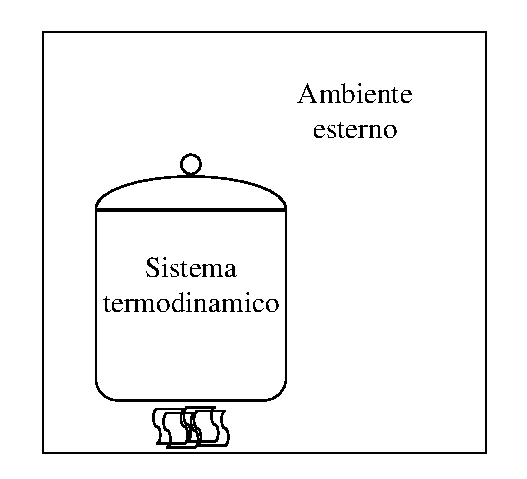
\includegraphics[width = \marginparwidth]{universo_termodinamico.pdf}
    \caption{Un esempio di universo, composto da un sistema termodinamico
    (la pentola) e un ambiente esterno (la stanza). Viene anche mostrato uno
    scambio di energia, mediato dal fuoco.}
    \label{pentola}
\end{marginfigure}


Possiamo classificare i sistemi termodinamici sulla base di due criteri: capacità
di scambiare materia e capacità di scambiare energia con l'ambiente esterno.

\begin{center}
    \begin{tabular}{c | c | c}
        Sistema & Scambia materia & Scambia energia \\
        \hline
        \hline
        \textit{Aperto} & $\surd$ & $\surd$ \\
        \hline
        \textit{Chiuso} & $\times$ & $\surd$ \\
        \hline
        \textit{Isolato} & $\times$ & $\times$
    \end{tabular}
\end{center}

\noindent È immediato chiedersi se esistono sistemi opposti a quelli chiusi, che
scambiano materia ma non energia con l'ambiente esterno. Ma questo
è impossibile, perché vale
\begin{align}
    E = mc^2
\end{align}
\noindent dove $c$ corrisponde alla velocità della luce nel vuoto.
Questa celebre equazione, anche se più complessa di quel che
sembra, mostra che ogni corpo possiede una certa energia $E$ per il semplice
motivo che esso possiede una massa $m$.

\subsection{Variabili termodinamiche}
Le \textit{variabili} (o \textit{coordinate}) \textit{termodinamiche}
sono gli strumenti che in termodinamica sostituiscono le proprietà
cinematiche a cui eravamo abituati in meccanica: lo spazio e il tempo,
che ci permettevano di descrivere il moto dei punti materiali.
Come già discusso precedentemente, questa sostituzione ha motivi pratici.
Le variabili termodinamiche fondamentali sono \textit{pressione} $p$
(rapporto tra il modulo di una forza perpendicolare ad una superficie
e l'area della superficie stessa), \textit{temperatura} $T$ (espressione
quantitativa della nostra sensazione di caldo e freddo), \textit{volume} $V$
e massa $m$\footnote{In termodinamica è spesso presente un'influenza da parte
della chimica, quindi alla massa si preferisce la \textit{mole} (come
la massa, si riferisce a quantità di materia).}. Come poi in cinematica
utilizzavamo un sistema di assi cartesiani, anche ora utilizziamo lo
stesso strumento matematico (il piano $pV$, pressione-volume) accoppiandolo però con le coordinate termodinamiche
appena introdotte. Il piano $pV$ sarà costituito da un solo quadrante,
perché sia il volume che la pressione possono assumere valori non
negativi\footnote{Anzi positivi, come accade spesso nella realtà.}.

Le variabili termodinamiche si suddividono in due categorie:
grandezze \textit{intensive} ed \textit{estensive}. Il valore delle
grandezze intensive non dipende dalla quantità di materia o dall'estensione
del campione esaminato, ma soltanto dalla sua natura e/o dalle
condizioni in cui si trova e possono essere misurate localmente.
La temperatura di una stanza, per esempio, non dipende dalle sue
dimensioni o dal tipo di aria che esso contiene. Dall'altro lato,
le estensive dipendono dalla quantità di materia esaminata e dalla
sua estensione.

\begin{center}
    \begin{tabular}{c || c}
        Grandezze intensive & Grandezze estensive\\
        \hline
        $p$, $T$ & $V$, $m$
    \end{tabular}
\end{center}


\subsection{Trasformazioni termodinamiche ed equilibrio}
I sistemi termodinamici possono essere descritti dalle coordinate
termodinamiche appena introdotte, che giacciono su un piano. Un
sistema che viene idealmente rappresentato da un punto fisso sul
piano $pV$ è in uno \textit{stato di equilibrio termodinamico},
nel quale le condizioni di pressione, volume e temperatura rimangono
costanti col passare del tempo.
Un sistema si dice in equilibrio termodinamico se esso rispetta i seguenti equilibri:
\begin{enumerate}
    \item \textit{Equilibrio meccanico}: lo stato non è sottoposto a forze totali non nulle,
    in qualsiasi coppia delle sue parti.

    \item \textit{Equilibrio chimico}: non esiste alcuna reazione chimica tra una qualsiasi
    coppia di parti del sistema.

    \item \textit{Equilibrio termico}: per ogni coppia di parti, la temperatura è la stessa.
\end{enumerate}

\noindent Per ``parti'' di un sistema intendiamo sottoinsiemi
abbastanza piccoli rispetto al sistema originale ma allo stesso
tempo sufficientemente grandi affiché gli strumenti della termodinamica
funzionino.


Un sistema può ovviamente muoversi all'interno del piano $pV$, cambiando
i propri parametri termodinamici e spostandosi tra due stati differenti.
Questi movimenti sono chiamati \textit{trasformazioni termodinamiche} e
vedremo più avanti che sono processi che coinvolgono scambi di energia
tra sistema termodinamico e ambiente esterno. Nel mondo reale, approssimare
sperimentalmente la curva di una trasformazione sul piano $pV$ è
estremamente difficile e dunque, se un sistema passa dallo stato $A$
ad uno differente $B$, non vi è garanzia di equilibrio nel percorso
tra i due punti. Per ora, ciò ci permette solo di ``accontentarci'' di
stimare teoricamente l'energia scambiata e i parametri in una trasformazione
termodinamica. Per questo motivo, sottointenderemo la seguente assunzione
in questo capitolo: tutte le trasformazioni trattate sono \textit{quasistatiche}\footnote{Da non confondere con le trasformazioni \textit{reversibili}, trattate più avanti.}
(a meno che non venga specificato diversamente).

\begin{tcolorbox}[colback = yellow!30, colframe = yellow!30!black, title = {Trasformazione quasistatica}]
    Trasformazione termodinamica ideale nella quale il sistema termodinamico
    attraversa equilibri successivi. Data una trasformazione $\tau$ quasistatica
    sul piano $pV$, tutti i punti di $\tau$ sono stati di equilibrio.
\end{tcolorbox}

\noindent Le trasformazioni quasistatiche sono irriproducibili sperimentalmente,
perché, affinché ad \textit{ogni} istante il sistema si trovi in uno stato
di equilibrio, è necessario variare le sue coordinate termodinamiche in
quantità infinitesime e in tempi sufficienetemente lunghi in modo da non
rompere gli equilibri.



\subsection{Quantificare caldo e freddo}
Abbiamo tutti un'idea intuitiva della temperatura, della quale facciamo
esperienza col tatto. Non tutti però percepiscono caldo e freddo allo
stesso modo e spesso non siamo bravi a stimare con precisione la
temperatura di un oggetto\footnote{\href{https://www.youtube.com/watch?v=vqDbMEdLiCs}{\textcolor{blue}{Misconception about Temperature - Veritasium}}.}.
Nella storia passata siamo riusciti ad individuare alcuni metodi in
grado di misurare indirettamente la temperatura, grazie agli effetti
della sua variazione. Il più comune di questi è la dilatazione dei
metalli. I vecchi e classici termometri a mercurio sfruttano questo
principio.

\begin{tcolorbox}[colback = yellow!30, colframe = yellow!30!black, title = {Termometro}]
Strumento che, data la variazione di una certa grandezza $X$ per
via di variazioni di temperatura, permette di misurare quest'ultima.
\end{tcolorbox}

...discorso su calibrazione ecc...

Se la misura che i termometri ci forniscono è indiretta, come possiamo
essere sicuri che il valore che otteniamo sia quello corretto? Il
principio zero, di cui si parla nella prossima sezione, ci consente di fidarci dei termometri.


\section{Principio zero}
\begin{tcolorbox}[colback = red!30, colframe = red!30!black, title = {Primo zero della termodinamica}]
Se un corpo $A$ è in equilibrio termico con $B$ e $B$ lo è con un terzo
corpo $C$, allora $A$ è in equilibrio termico con $C$.

In particolare, se $T_A = T_B$ e $T_B = T_C$, allora $T_A = T_C$; cioè
i corpi possiedono la medesima temperatura.
\end{tcolorbox}

\noindent Sottolineamo che le equivalenze espresse dal principio non
sono dedotte da proprietà logico-matematiche, ma sono affermazioni
forndate puramente su evidenze sperimentali.

Alcuni testi espongono il principio zero anticipando un fatto dell'universo
che noi affrontiamo nella seconda parte, cioè che due corpi, uno caldo e
uno freddo, in contatto termico tra loro raggiungeranno la stessa temperatura,
se si attende un tempo sufficientemente lungo. Precisiamo che l'equilibrio
termico, nel mondo reale, è un equilibrio dinamico. Ciò significa che
la temperatura di due corpi in contatto termico non è sempre esattamente la
stessa, ma può subire microscopiche fluttuazioni che tuttavia si possono
spesso trascurare.


\section{Esperienza di Joule}
A metà del Diciannovesimo secolo, James Prescott Joule compì alcuni
esperimenti celebri che misero in luce il legame tra alcune forme di
energia e temperatura. Il più noto esperimento è quello del mulinello,
con il quale Joule mostrò \textit{l'equivalente meccanico del calore}.
Il dispositivo di Joule consisteva in un serbatoio adiabatico contenente
acqua, la cui temperatura veniva controllata per mezzo di un termometro
infilato in un'apertura del serbatoio. Nell'acqua vi era poi immerso
un mulinello azionato dall'esterno da un sistema di carrucole e masse
in caduta libera. L'esperimento consisteva nel sollevare una certa
massa totale $m$ ad una altezza $h$; cadendo, la massa avrebbe messo
il mulinello in rotazione, agitando l'acqua del serbatoio. Joule
osservò che la temperatura dell'acqua aumentava dopo la caduta della
massa e l'incremento di temperatura era proporzionale alla massa e all'altezza.

Un'analisi energetica del sistema mette in luce che un certo lavoro è
stato compiuto sull'acqua del serbatoio:

\[ W = mgh \]

\noindent Per principio di conservazione dell'energia, il lavoro non
può essere sparito nel nulla. L'effetto della caduta della massa è stato però un aumento di temperatura.
La conclusione più ragionevole è che temperatura ed energia sono tra
loro legati da qualche relazione.




\section{Principio primo}
Con il primo principio della termodinamica introduciamo una semplice
legge che descrive le modalità con le quali i sistemi dell'universo
comunicano tra loro, cioè come essi scambiano energia. Non a caso
esponiamo dettagliatamente in questa sezione i tre meccanismi
principali con i quali il calore si ``muove'' (conduzione, convezione,
irraggiamento).


\subsection{Lavoro ed energia interna}
Come abbiamo osservato con Joule, è sperimentalmente evidente che
se si compie lavoro sull'acqua, essa
aumenta la propria temperatura. Inoltre, se la temperatura iniziale
dell'acqua è la stessa in tutti gli esperimenti e il lavoro compiuto
è sempre uguale, allora la temperatura finale sarà anch'essa la stessa
in tutte le situazioni. Da ciò si può dedurre che l'aumento di
temperatura non dipende dalla natura del lavoro. Cos'è allora la
temperatura? Non possiamo ancora rispondere a questa domanda, ma
sicuramente sappiamo che essa è legata in qualche modo all'energia,
quantomeno al lavoro.

La temperatura ci fornisce un'informazione sullo stato di
un corpo, cioè una proprietà che lo caratterizza in un dato istante,
in una certa situazione. Il lavoro è invece qualcosa di dinamico,
una ``energia in movimento'' dovuta al moto di qualche cosa. Il
lavoro si trasferisce da corpo a corpo e ne altera una proprietà di
stato, il cui indicatore è la temperatura. L'energia del lavoro,
allora, si può immagazzinare nei corpi, come abbiamo visto parlando
di (variazione di) energia potenziale $\Delta\mathcal{U} = -W$.
Anche qui potremmo parlare di una qualche energia potenziale, ma
non possiamo denominarla in questo modo perché in generale non
si osservano forze conservative in azione. Introduciamo allora
l'energia interna di un sistema, che, come si è osservato
dagli esperimenti, è esprimibile come funzione della temperatura

\[ U = U(T) \]

\noindent Non possiamo ancora dire con precisione quale sia
la formula chiusa che unisce le due quantità, ma sicuramente
gli esperimenti confermano che energia interna e temperatura
sono legate da una qualche costante di proporzionalità:

\[ U \propto T \]

\subsection{Calore}
Dal paragrafo precedente abbiamo scoperto che si può dedurre il
contenuto energetico di un sistema in funzione della sua temperatura.
Con Joule, però, abbiamo visto che, per aumentare la temperatura di
un sistema, è necessario compiere del lavoro su di esso. Ma per
esperienza sappiamo che un corpo freddo può essere riscaldato da uno
più caldo. In una situazione del genere, tuttavia, non si osserva alcun lavoro in azione. Per
spiegare questo fenomeno, la fisica ha introdotto una quantità
energetica nuova: il calore.

\begin{tcolorbox}[colback = red!30, colframe = red!30!black, title = {Calore}]
Energia scambiata tra corpi con temperature differenti in contatto termico\footnote{Per esperienza sappiamo che il passaggio spontaneo avviene
dal corpo più caldo a quello più freddo, ma questa proprietà della natura viene riassunta in principi della termodinamica che affronteremo più avanti.}.

Spesso indicata con $Q$.
\end{tcolorbox}

Spesso si è tentati di associare il calore alla temperatura. Si
tratta di un'idea errata, perché la temperatura rappresenta lo
stato di un sistema, mentre il calore è solo energia in movimento,
come lo è il lavoro. Queste grandezze si manifestano solamente
durante trasferimenti di energia. Il legame tra temperatura e calore
è tuttavia molto stretto:

\[ \Delta T \propto Q \]

\noindent cioè il calore corrisponde ad una certa variazione della temperatura
del sistema. In altri termini, variazione di temperatura e calore sono legati
mediante una certa costante $\xi$ dalla relazione $\Delta T = \xi Q$.

Abbiamo visto come quantificare la temperatura mediante i termometri. Rimane
però il problema di come quantificare il calore. Per fare un
esempio concreto, supponiamo di voler scaldare un salotto con una stufa. Per
incrementare la temperatura della stanza da 200 K a 300 K, sarà necessario
bruciare una certa quantità di legna. È facile allora esprimere il calore
necessario (che è l'energia sprigionata dalla legna che arde) ad aumentare
la temperatura della stanza: È proprio funzione della quantità di legna che dobbiamo
comprare e bruciare, a meno della costante $\xi$ espressa precedentemente.

Se anche il calore, come il lavoro, può variare la temperatura di un sistema,
ciò implica che anche lo scambio di calore può mutare l'energia interna di
un sistema.
Abbiamo visto precedentemente che l'energia interna di un sistema è una qualche
funzione della temperatura, $U = U(T)$. Questa relazione si suppone essere
invertibile, $T = T(U)$. Dagli studi sul calore, poi, abbiamo mostrato la
relazione tra calore e variazione di temperatura, dalla quale possiamo notare
che

\[ Q = \frac{1}{\xi}\Delta T = \frac{1}{\xi}(T_f - T_i) = \frac{1}{\xi}(T(U_f) - T(U_i)) \]

\noindent A meno di costanti, possiamo esprimere il calore come quantità
proporzionale alla variazione di energia interna del sistema:

\[ Q \propto \Delta U \]


\subsection{Capacità termica e calore specifico}
Esistono definizioni che ci permettono di quantificare il calore
``ad alto livello\footnote{Nel senso informatico (eh pefforza
d'altronde questo corso è dedicato agli informatici).}'', ovvero
ricorrendo a misure che non richiedono di conoscere la struttura
interna, potenzialmente microscopica, del sistema (in effetti
è proprio così che funziona la termodinamica).

Già nel paragrafo
precedente ci siamo posti implicitamente questa domanda: come
quantificare il calore? Sappiamo che $Q \propto \Delta T$.
Questa relazione di proporzionalità ci permette di definire una
proprietà dei corpi, che è la capacità termica.

\begin{align}
    C_\gamma \eqdef \left[ \frac{dQ}{dT} \right]_\gamma
\end{align}

\noindent In breve, la costante $C_\gamma$ esprime la quantità di calore
necessaria per aumentare la temperatura di un corpo di una
certa differenza $dT$. In casi ideali, possiamo semplificare
questa legge in $Q = C_\gamma \Delta T$. La $\gamma$ indica che
la capacità termica è sempre associata ad una certa trasformazione
termodinamica $\gamma$ e non è necessariamente uguale in ogni
situazione.

Già intuitivamente possiamo capire che più il corpo è grande,
nel senso che possiede più massa, più calore sarà richiesto per
aumentare la sua temperatura. Sempre in base alla trasformazione,
possiamo allora definire il calore specifico:

\begin{align}
    c_\gamma \eqdef \frac{C_\gamma}{m}
\end{align}

\noindent da cui una formula che più avanti si incontra spesso:
$Q = mc_\gamma \Delta T$. Queste costanti non solo dipendono da
$\gamma$, ma variano anche da sostanza a sostanza. Il calore
specifico di un metallo è generalmente più basso di qualcosa
come l'acqua, principalmente per questione di conducibilità termica,
di cui parliamo più avanti.


\subsection{Formulazione del primo rincipio}
Possiamo ora mostrare il primo principio della termodinamica. Il principio
mostra semplicemente che un sistema può variare la propria energia interna
mediante il contributo energetico di due quantità ``in movimento'': il lavoro,
$W = -\Delta U_W$\footnote{Poniamo il segno negativo per convenzione e convenienza matematica, come abbiamo fatto per l'energia potenziale.}
e il calore scambiato con l'ambiente, $Q = \Delta U_Q$. Questi contributi si sommano per deterimanre una
variazione totale $\Delta U = \Delta U_Q  + \Delta U_W$, da cui la formulazione
seguente del primo principio:

\begin{align}
    \Delta U = Q - W\label{firstprincip}
\end{align}

\noindent Sarebbe più corretto mostrare la seguente forma differenziale

\begin{tcolorbox}[colback = red!30, colframe = red!30!black, title = {Primo principio della termodinamica}]
\begin{align}
    dU = \delta Q - \delta W
\end{align}
\end{tcolorbox}

\noindent Ci limetermo alla seguente interpretazione: $d$ rappresenta
un differenziale esatto, che sottolinea l'indipendenza della differenza
dal percorso. La differenza di energia interna $dU$ dipende solo dagli
stati iniziale e finale del sistema, ignorando ciò che è accaduto durante la
trasformazione.
Il simbolo $\delta$ indica invece che i contributi di calore e lavoro
possono essere differenti a seconda della trasformazione
avvenuta. In altre parole, la stessa differenza $dU$ può aver
avuto origine da trasformazioni termodinamiche differenti, ognuna
delle quali ha osservato un diverso contributo di lavoro e calore.
Per riassumere, \textit{l'energia interna definisce una proprietà
di stato del sistema} e invece \textit{calore e lavoro sono proprietà
della particolare trasformazione}.

\begin{marginfigure}
    \centering
    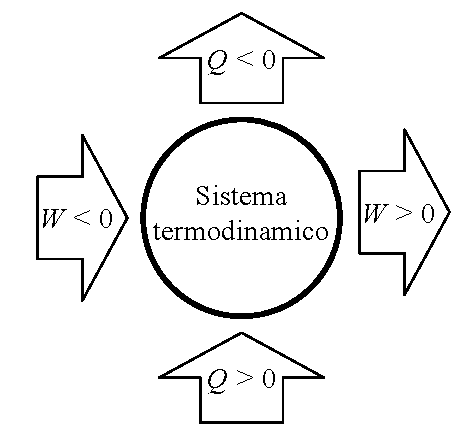
\includegraphics[width = \marginparwidth]{convenzione_segni_flussi_energetici_sistema_termodinamico.pdf}
    \caption{Convenzione sui segni dei flussi energetici in un
    sistema termodinamico, al quale si applica la nostra
    formulazione del primo principio.}\label{fluxi}
\end{marginfigure}

Chiariamo le convenzioni sui segni: supponiamo di avere un sistema
termodinamico che scambia calore con l'ambiente e che può compiere
lavoro. La situazione è mostrata in figura \ref{fluxi}.
Quando il sistema acquista calore dall'ambiente esterno,
il valore di questà quantità sarà positivo. Quando invece il
sistema perde calore, quest'ultimo ha valore negativo. In accordo
con il primo principio, supponendo di ignorare il lavoro, l'energia
interna $U$ del sistema diminuisce quando il calore esce e viceversa
aumenta quando entra nel sistema.
Per il lavoro vale il contrario: quando l'ambiente effettua lavoro
sul sistema, questa quantità di energia in entrata ha valore negativo;
quando invece il sistema effettua lavoro sull'ambiente, esso spende
e perde parte della sua energia interna. Per questo motivo, nel
primo principio, il lavoro viene sottratto alla variazione di energia
totale.

Sottolineamo infine che, nella formulazione \ref{firstprincip},
$\Delta U$ corrisponde alla variazione \textit{totale} di energia
interna del sistema in un dato momento nel quale avviene scambio
di energia. Sono dunque totali anche il calore scambiato
$Q$ e il lavoro effettuato $W$.


\subsection{Modalità di trasmissione del calore}
Come il lavoro può presentarsi in svariate forme, come abbiamo
visto dagli esperimenti di Joule ma già anche dalla meccanica,
anche il calore può essere scambiato in vari modi. Queste modalità
di trasmissione hanno in comune la condizione di \textit{contatto
termico}, ovvero situazioni in cui due corpi sono in grado di
trasmettere calore tra di loro. È importante non confondere il
contatto termico con quello fisico, perché, come vedremo, non
sempre il calore si trasmette solo se due corpi si toccano tra loro.

Altro punto da ricordare è che possiamo distinguere che l'energia
si trasferisce sotto forma di calore perché non si compie lavoro.

\subsubsection{Conduzione}
Nella conduzione, il calore viene scambiato per contatto tra corpi.
Un semplice modello per descrivere questo fenomeno è la finestra di
un edificio.

\subsubsection{Convezione}
Nella convezione, il calore viene scambiato per mezzo di masse calde
in movimento, all'interno di masse più fredde. Questa modalità è
caratteristica dei fluidi, data la necessità del moto. Semplici esempi
di questo fenomeno sono la pentola d'acqua sul fornello acceso e la
lava-lamp.

\subsubsection{Irraggiamento}
L'irraggiamento permette lo scambio di energia per mezzo di onde
elettromagnetiche, quindi senza la necessità di essere in contatto
termico con un corpo. Un esempio è il Sole, che di fatto scalda la
Terra mediante le radiazioni emesse. In realtà non è propriamente
corretto dire che il calore viene trasmesso durante il tragitto tra
i due corpi, ma l'effetto delle onde elettromagnetiche che raggiungono
la destinazione è un aumento di temperatura, che assimiliamo ad uno
scambio di calore.

Una legge degna di nota è la \textit{legge di Stefan-Boltzmann} del
potere emissivo di un corpo

\begin{align}
    \varepsilon = \sigma e T^4
\end{align}

\noindent Questa legge esprime la quantità di energia che un corpo
può emettere per irraggiamento data la sua temperatura. Nella realtà,
un corpo non è in grado di emettere la totalità di questa energia
e per tale motivo è presente un fattore $e$ adimensionale, tale che
$0 < e < 1$. Nel caso ideale $e = 1$ si parla di \textit{corpo nero}.
La quantità

\section{Gas ideali}

\subsection{Leggi dei gas ideali}

\subsubsection*{Prima legge di Gay-Lussac}
\subsubsection*{Seconda legge di Gay-Lussac}
\subsubsection*{Legge di Boyle}

\subsubsection*{Legge di Avogadro}
Esempio di equazione di stato.

\subsection{Lavoro di un gas ideale}
Mostreremo ora parte del principio di funzionamento di un pistone
di un motore a combustione interna. Si tratta di un esempio estremamente
semplificato, perché considereremo gas ideali.
Sappiamo bene che il motore termico di, ad esempio, una motocicletta
genera lavoro per azionare la catena e di conseguenza la ruota posteriore.
Il ``tempo'' nel quale il motore genera lavoro è quello nel quale
avviene lo scoppio, che aumenta violentemente la temperatura e la
pressione dell'aria all'interno del cilindro, spingendo di fatto il
pistone.

\begin{marginfigure}
    \centering
    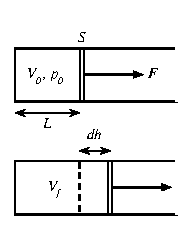
\includegraphics[width = \marginparwidth]{lavoro_gas_ideale.pdf}
    \caption{Lavoro infinitesimo di un gas all'interno di un cilindro.}
    \label{workinggas}
\end{marginfigure}

Si faccia riferimento al motore in figura \ref{workinggas}, costituito
da un cilindro e un pistone libero di muoversi al suo interno. Inizialmente, il pistone,
con sezione di area $S$, si trova ad una distanza $L$ dal fondo del cilindro.
L'aria all'interno ha pressione e volume iniziali $p_0$ e $V_0$. Se l'esterno
del pistone oppone resistenza, il gas del cilindro, avendo una certa pressione,
esercita sulla sezione del pistone una certa forza $\vecsymb{F}$. Immaginiamo
che la resistenza esterna cessi ad un certo istante: il gas, in virtù della forza
esercitata, spingerà il pistone di una certa distanza infinitesima $dh$.
Il gas sta allora compiendo lavoro sul pistone:

\[ dW = \vecsymb{F} \cdot d\vecsymb{s} = Fdh \]

\noindent la forza $F$ non ci è molto utile attualmente. Vogliamo esprimere
tutto sotto forma di variabili termodinamiche e non meccaniche. Notiamo
allora che, dopo lo spostamento $dh$, il gas raggiungerà un certo volume
$V_f$, che è leggermente più voluminoso di $V_0$ di una certa quantità $dV$:

\[ V_f = (L + dh)S = SL + Sdh = V_0 + dV \]

\noindent Tramite semplice algebretta, possiamo dedurre che
$dW = Fdh = \frac{F}{S}Sdh = pdV$. Abbiamo dunque definito
il lavoro infinitesimo di un gas ideale

\begin{align}
    dW = pdV
\end{align}

Stiamo assumendo che, durante l'aumento di $dV$, la pressione
rimanga costante. Se però vogliamo calcolare il lavoro totale
sprigionato durante l'intera corsa del pistone, dobbiamo effettuare
un'integrazione tenendo presente che la pressione varierà durante
tale processo. In generale, data una certa trasformazione termodinamica
$\tau$, il lavoro totale di un gas può essere espresso nella
seguente forma:

\begin{align}
    W_\tau = \int_\tau pdV\label{lavorogas}
\end{align}

\subsubsection*{Il lavoro sul piano $pV$}
Sappiamo bene dalla quinta superiore e da Analisi 1 che gli integrali
sono in qualche modo correlati a interpretazioni geometriche di aree
sottese a grafici. Dalla legge \ref{lavorogas} ottenuta pocanzi si può
notare che il lavoro ``si può vedere'' sul piano $pV$. Dato infatti
il tratto di curva $\tau$ che descrive una trasformazione, il lavoro
$W$ è proprio l'area (con segno) sottesa a $\tau$. In generale,

\begin{itemize}
    \item se il sistema percorre $\tau$ in modo tale da spostarsi nel verso positivo
    dell'asse del volume, il lavoro effettuato dal gas è positivo;

    \item se il sistema si dirige nel verso opposto dell'asse del volume,
    allora il lavoro effettuato è negativo;

    \item se il sistema non si discosta dal proprio volume ($dV = 0$)
    allora il lavoro è nullo.
\end{itemize}

Anticipiamo che esistono trasformazioni particolari, le trasformazioni
\textit{cicliche}, che partendo da una coordinata termodinamica
ritornano sulla medesima dopo la trasformazione, descrivendo un circuito.
In tal caso, il lavoro effettuato dal (o sul) sistema corrisponde
all'area racchiusa nel circuito. La figura mostra intuitivamente le
ragioni di questa proprietà.

\begin{itemize}
    \item Se il sistema percorre il circuito in senso orario, il
    lavoro è positivo.

    \item Se il sistema percorre il circuito in senso antiorario,
    il lavoro è negativo.
\end{itemize}





\subsection{La teoria cinetica dei gas}
È evidente che, nella termodinamica da noi affrontata, il sistema
fisico preferito è quello del gas. Lo abbiamo però sempre trattato
da un punto di vista macroscopico, utilizzando variabili termodinamiche
(pressione, volume e temperatura), senza mai spiegare cosa in realtà
accade nel microscopico, all'interno del gas stesso. È ciò che proveremo
a fare ora, costruendo una teoria che spieghi ciò che osserviamo
dall'esterno. Non abbiamo però altro strumento che quello della meccanica
e per questo motivo i risultati che otterremo in seguito sono
conosciuti sotto il nome di \textit{teoria cinetica dei gas}.

\subsubsection*{Ipotesi e presupposti della teoria}
Sottolineamo che la teoria cinetica, per funzionare, poggia su numerosi
presupposti, molti dei quali sono solo un'approssimazione della realtà.
Tuttavia, vedremo che queste ipotesi condurranno ad una spiegazione
soddisfacente delle nostre osservazioni:

\begin{itemize}
    \item Oggetto della trattazione teorica è un \textit{gas ideale}
    (o perfetto) che si trova all'interno di un contenitore con
    volume $V$. La forma del contenitore non sarà rilevante, ma spesso
    si semplificano i calcoli se esso è un cubo.

    \item Il gas è ideale nel senso che esso è costituito da particelle
    infinitamente piccole rispetto al contenitore e alle distanze che
    le separano. Tali particelle sono inoltre indistinguibili l'una
    dall'altra (eccezion fatta per il loro stato di moto): esse hanno
    in particolare la medesima massa.

    \item Sempre il gas è ideale in quanto a bassa pressione e densità,
    nella misura in cui l'interazione tra le particelle è nulla: non
    avvengono urti e non vi sono interazioni di natura gravitazionale,
    elettrica o di altro genere.

    \item Gli unici urti non trascurabili sono quelli che avvengono
    tra particella e parete del contenitore ed essi sono perfettamente
    elastici, perché tra l'altro la massa delle particelle è infinitamente
    piccola rispetto a quella del contenitore e delle sue pareti. L'urto
    non mette dunque in moto il contenitore.
\end{itemize}

\subsubsection*{La teoria}
Coerentemente con le ipotesi espresse nel paragrafo precedente,
consideriamo ora una singola particella del gas ideale, con massa
$m$. Esso sta per urtare una parete del contenitore cubico, con
lato $L$ e di una certa massa $M$ tale che $M \gg m$. Proiettiamo la situazione su un piano, come in figura
\ref{wall}. La particella potrebbe avere una qualsiasi velocità,
che denoteremo $\vecsymb{v}$. Consideriamo poi solo la componente
orizzontale di tale vettore, ovvero $\vecsymb{v}_x$.

%\begin{marginfigure}
%    \centering
%    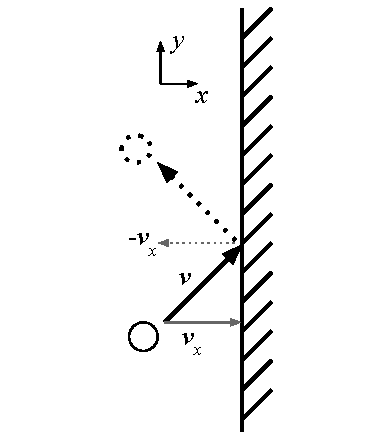
\includegraphics[width = \marginparwidth]{teoria_cinetica_parete.pdf}
%    \caption{Urto tra una particella di gas e una delle pareti
%    del contenitore.}
%    \label{wall}
%\end{marginfigure}

\begin{marginfigure}
    \begin{center}
        \begin{tikzpicture}

            \filldraw[black] (0,0) circle (2pt) node[below right]{$m$};
            \filldraw[black] (2,2) circle (2pt) node[below right]{};
            \filldraw[black] (0,4) circle (2pt) node[below right]{};

            \draw[->] (0.2,0.2) -- (1.8,1.8);
            \draw (1,1) node[above left]{$\vecsymb{v}_i$};

            \draw[->] (1.8,2.2) -- (0.2,3.8);
            \draw (1,3) node[above right]{$\vecsymb{v}_f$};

            %wall
            \draw (2,0) -- (2,4);
            \fill[pattern=north west lines] (2,0) rectangle ++(1,4);
        \end{tikzpicture}
    \end{center}
    \caption{Urto tra una particella di gas e una delle pareti
    del contenitore.}
    \label{wall}
\end{marginfigure}

Sappiamo dalle equazioni \ref{perfelastico} che l'urto perfettamente
elastico farà rimbalzare la particella in modo tale da rendere
invariato il modulo di $\vecsymb{v}_x$, ma invertendone il verso.
Le quantità di moto finale e iniziale della particella, allora,
corrispondono rispettivamente a $\vecsymb{p}_{x,i} = m\vecsymb{v}_x$
e $\vecsymb{p}_{x,f} = -m\vecsymb{v}_x$. La variazione della quantità
di moto della particella è quindi

\[ \Delta\vecsymb{p}_x = -2mv_x \hat{x} \]

\noindent Utilizziamo il versore $\hat{x}$ per separare i moduli e per trattare
oggetti scalari.

Sappiamo che la variazione $\Delta\vecsymb{p}_x$ può essere interpretata
come un impulso esercitato dalla parete, che quindi esercita una forza
sulla particella. Ma come calcolare questa forza? È necessario trovare
un intervallo temporale entro il quale l'impulso agisce, in modo da
ricavare l'intensità della forza mediante la definizione \ref{impulso}.
Possiamo notare che, per via degli urti perfettamente elastici, la particella
continua a rimbalzare senza che la sua velocità totale $v$ muti.
Proiettando il moto sull'asse $x$, vedremmo il vettore $\vecsymb{v}_x$
invertirsi ciclicamente ad ogni urto con le pareti di destra e sinistra.
La particella impiega allora un tempo

\[ \Delta t = \frac{2L}{v_x} \]

\noindent per lasciare una parete e tornarvici per urtare nuovamente.
Durante questo intervallo di tempo, in media, la forza impulsiva
esercitata da una parete sulla particella ha intensità

\[ F_x = \frac{\Delta p_x}{\Delta t} = 2mv_x \frac{v_x}{2L} = \frac{mv_x^2}{L} \]

\noindent Tramite la definizione di pressione $p = F/S$, (con $S$ la
superficie di una parete, dunque $L^2$) otteniamo la
pressione esercitata dalla singola particella

\[ p_x = \frac{F_x}{L^2} = \frac{mv_x^2}{L^3} = \frac{mv_x^2}{V} \]

\noindent Notare che questo ragionamento vale solo per la componente
$x$, ma lo stesso ragionamento può essere esteso a tutte le altre
componenti. La relazione precedente non è ancora di nostro aiuto,
perché riguarda solo una particolare particella, la cui velocità può
essere differente dalle altre. Calcoliamo dunque la pressione mediante
la forza totale esercitata dalle particelle sull'asse $x$:

\[ F_{\text{tot}, x} = \sum_i F_{x,i} = \sum_i \frac{mv_{x,i}^2}{L} = \frac{m}{L}\sum_i v_{x,i}^2 \]

Supponendo che il gas sia costituito da $N$ particelle, possiamo
effettuare un'approssimazione riducendo le velocità ad una loro media
(essendo al quadrato, sarà una velocità quadratica media).

\[ p_x = \frac{F_{\text{tot},x}}{L^2} = N\frac{m\left\langle v_x^2 \right\rangle}{V} \]

Il ragionamento effettuato per la componente $x$ vale anche per tutte
le altre. Per questo motivo, dato che la pressione è una grandezza
intensiva che idealmente rimane costante in tutto il cubo, possiamo
supporre che $p_x = p_y = p_z = p$. Vogliamo però ottenere un'equazione
che non dipenda da una componente della velocità delle particelle,
ma dalla loro velocità totale. Anche qui supponiamo di ridurre le
velocità di tutte le particelle, che potrebbero differire tra loro,
ad una velocità quadratica media totale. La relazione con le sue
componenti spaziali è ricavabile geometricamente:

\[ \left\langle v^2 \right\rangle  = \left\langle v_x^2 \right\rangle + \left\langle v_y^2 \right\rangle + \left\langle v_z^2 \right\rangle \]

\noindent Le approssimazioni introdotte ci permettono anche di
supporre che tutte e tre le componenti spaziali siano equivalenti
tra loro, ovvero che $\left\langle v_2^2 \right\rangle = \left\langle v_y^2 \right\rangle = \left\langle v_z^2 \right\rangle$.
Usando allora l'equazione della pressione:

\[ p = N\frac{m}{V}\left(\frac13 \left\langle v^2 \right\rangle\right) \]

\noindent Notiamo che compare il prodotto $m\left\langle v^2 \right\rangle$, che
corrisponde al doppio dell'energia cinetica media delle particelle,
$\left\langle E_K \right\rangle$. Otteniamo dunque la seguente relazione:

\[ pV = \frac23 N\left\langle E_K \right\rangle \]

\noindent $\left\langle E_K \right\rangle$ corrisponde ad una singola particella.
Allora possiamo concludere che la somma di tutte le energie cinetiche
medie delle particelle del gas costituiscono l'energia interna del
gas stesso: $E_\text{int} = U = N\left\langle E_K \right\rangle$.
La teoria ci ha dunque permesso dunque di unire le seguenti relazioni:

\[ pV = Nk_BT = \frac23 U \]

In particolare, possiamo notare che

\[ \left\langle E_K \right\rangle = \frac{3}{2}k_B T \]

\noindent che esprime la relazione tra energia cinetica media di una
particella e la temperatura. In un certo senso, la temperatura \textit{è}
l'energia cinetica media delle particelle.

\subsubsection*{Conclusioni}
Il risultato più importante della teoria cinetica è l'unione tra
il mondo macroscopico osservato sperimentalmente e il mondo microscopico
modellato teoricamente. In particolare:
\begin{itemize}
    \item La teoria cinetica offre una spiegazione dell'origine della
    pressione esercitata da un gas in un contenitore. L'origine è proprio
    dovuta alla continua collisione delle particelle con le pareti
    del contenitore.

    \item La teoria cinetica mostra che la temperatura è strettamente
    legata all'energia cinetica media delle particelle. Intuitivamente,
    la temperatura è interpretabile proprio come l'agitazione media
    delle particelle, per l'appunto l'energia del loro movimento.

    \item La teoria cinetica costruisce un modello generalizzabile
    a sistemi di costituenti non necessariamente monoatomico-puntiformi,
    come approfondito nella prossima sezione.
\end{itemize}

\subsubsection*{Gradi di libertà}
Nell'equazione relativa all'energia cinetica media,
il fattore $1/2$ deriva dalla definizione di enrgia cinetica, ma
il numero $3$ invece? Esso dipende dal numero di dimensioni entro
le quali le particelle possono muoversi, ovvero i \textit{gradi di
libertà}. Se compissimo lo studio da capo, costringendo però le particelle
a giacere su un piano, i gradi di libertà sarebbero solo due e il fattore
moltiplicativo
dell'energia cinetica media sarebbe diverso. Ciò è dovuto al fatto
che ogni grado di libertà permette alla particella di muoversi su
un'altra dimensione e quindi di aggiungere un contributo in più alla
propria energia cinetica. In generale, ogni grado di
liberta comporta un contributo energetico di $\frac12k_BT$ e
dunque, per $l$ gradi di libertà, si ottiene

\begin{align}
    \left\langle E_K \right\rangle = \frac{l}{2}k_BT
\end{align}

I gradi di libertà possono crescere all'aumentare della complessità
della particella di gas. Oltre alle tre dimensioni, una molecola
biatomica (quindi non puntiforme come abbiamo sempre supposto finora)
può anche ruotare su due assi\footnote{Due assi sono sufficienti a
coprire tutte le rotazioni nelle tre dimensioni}; i due atomi possono
poi vibrare intorno alla loro ``sede'' nella molecola, dunque anche
questa energia deve essere presa in considerazione. In totale, una
molecola biatomica ideale può avere $l = 6$ gradi di libertà.






\section{Trasformazioni termodinamiche}
Questa sezione è dedicata ad analisi più approfondite sulle trasformazioni
termodinamiche fondamentali, ovvero trasformazioni molto semplici da
trattare mediante gli strumenti di termodinamica finora mostrati. Da
un certo punto di vista, queste trasformazioni rappresentano le modalità
fondamentali con le quali un sistema può muoversi sul piano $pV$. Un
motivo della loro semplicità risiede nel fatto che, in ogni trasformazione,
un qualche parametro termodinamico rimane sempre costante.

Supporremo che queste trasformazioni riguarderanno un gas ideale
contenuto in un cilindro. A seconda del caso di studio, il cilindro
potrà variare il proprio volume interno grazie ad un pistone mobile,
oppure sarà adiabatico. Le trasformazioni saranno inoltre \textit{quasistatiche
reversibili}: ad ogni istante, il sistema è in uno stato di
equilibrio (il passaggio dall'uno all'altro è sufficientemente lento
per raggiungere tale scopo) e inoltre è sempre possibile ripercorrere
la trasformazione, e ogni suo tratto intermedio, in senso inverso.
Le leggi che deriveremo non saranno pertanto applicabili alla lettera
a trasformazioni reali di gas reali, ma costituiranno solo una buona
approssimazione delle osservazioni sperimentali.


\subsection{Isocore}
Queste trasformazioni traggono il loro nome per via del loro volume,
che rimane sempre costante, cioè $dV = 0$. Segue in particolare che
$dW = pdV = 0$, ricordando la definizione di lavoro di un gas ideale.
D'altronde, il volume del gas non cambia e quindi nessuna parte del
suo contenitore viene mossa.

Dal primo principio vale $dU = dQ$. Ciò significa che avviene solo
scambio di calore. Possiamo supporre che il gas, durante la trasformazione,
vari la propria temperatura in relazione al calore scambiato secondo
un certo \textit{calore specifico a volume costante} $c_V$.

\begin{align}
    dQ = nc_VdT
\end{align}

\begin{marginfigure}
    \begin{center}
        \def\xmax{3}
        \def\ymax{2.5}
        \begin{tikzpicture}

        \coordinate (B) at (.5*\xmax,.8*\ymax);
        \coordinate (A) at (.5*\xmax,.2*\ymax);
        
        % LINE
        \draw[very thick,midarr=.55,myred] (A) -- (B);
        \fill (B) circle(0.07) node[right=2,above=2] {$B$};
        \fill (A) circle(0.07) node[right=2] {$A$};
        
        % AXIS
        \draw[->,thick] (0,-0.1*\ymax) -- (0,\ymax) node[anchor=north east] {$p$};
        \draw[->,thick] (-0.1*\xmax,0) -- (\xmax,0) node[anchor=north east] {$V$};
        
        \end{tikzpicture}
    \end{center}
    \caption{Trasformazione isocora sul piano $pV$. Il grafico evidenzia
    molto bene il fatto che il lavoro è nullo, proprio perché il tratto
    $AB$ descrive un segmento verticale che sottende area nulla (volgarmente, non
    ha largezza).}
\end{marginfigure}

\noindent Da cui $dU = nc_VdT$. Come aveva previsto Joule, per questa
particolare trasformazione abbiamo individuato una relazione che lega
energia interna e (variazione di) temperatura di un gas. Ricordando
poi la teoria cinetica, $U = \frac32 nRT$. È facile allora scoprire
che, dati $l$ gradi di libertà per un gas ideale,

\[ c_V = \frac{l}{2}R \]

\noindent per gas monoatomici in tre dimensioni, vale perciò $c_V = \frac32 R$.


\subsection{Isobare}
In queste trasformazioni, è la pressione a rimanere costante.
Calcolarne il lavoro è molto semplice. Si evince infatti che
la definizione si riduce ad una semplice moltiplicazione:
$dW = pdV$, da cui $W = p\Delta V$.

Dalle trasformazioni isocore, abbiamo scoperto un legame tra
variazione di energia interna del gas e variazione di temperatura.
Già per definizione legammo in una funzione queste due quantità.
In particolare, sptabilimmo che $U$ è una funzione di stato, la
cui variazione non dipende dal percorso ma dagli stati iniziale
e finale. Siamo allora legittimati a impiegare la relazione
$dU = nc_VdT$ trovata nelle isocore.

Rimane da trovare il calore scambiato durante una isobara. Anche
qui possiamo inventare una nuova costante, un \textit{calore specifico
a pressione costante} $c_p$, col quale legare calore e intervallo
di temperatura:

\[ dQ = nc_pdT \]

\noindent come per $c_p$, ci piacerebbe conoscere la sua vera forma.
Notiamo che differenziando i membri della legge di Avogadro,
$d[pV] = d[nRT]$, ci ritroveremo con la relazione $pdV = nRdT$,
da cui scopriamo che $dW = nRdT$. Dal primo principio $dU = dQ - dW$,
possiamo allora scoprire che $nc_VdT = nc_pdT - nRdT$, da cui
la \textit{relazione di Mayer}\footnote{Come lo studentato.}

\begin{marginfigure}
    \begin{center}
        % PV diagram - constant P
        \def\xmax{3}
        \def\ymax{2.5}
        \begin{tikzpicture}
        
        % AREA
        \coordinate (A) at (.2*\xmax,.6*\ymax);
        \coordinate (B) at (.8*\xmax,.6*\ymax);
        \coordinate (C) at (.8*\xmax,.2*\ymax);
        \fill[mylightblue] (A) rectangle (C|-0,0) node[midway,blue] {$W$};
        
        % LINE
        \draw[very thick,midarr=.55,myred] (A) -- (B);
        %\draw[very thick,midarr=.55,blue] (B) -- (C);
        \fill (A) circle(0.07) node[right=2,above=2] {$A$};
        \fill (B) circle(0.07) node[right=2,above=2] {$B$};
        %\fill (C) circle(0.07) node[right=2] {$P_2$, $V_2$};
        
        % AXIS
        \draw[->,thick] (0,-0.1*\ymax) -- (0,\ymax) node[anchor=north east] {$p$};
        \draw[->,thick] (-0.1*\xmax,0) -- (\xmax,0) node[anchor=north east] {$V$};
        
        \end{tikzpicture}
    \end{center}
    \caption{Trasformazione isobara sul diagramma $pV$. La
    pressione in $A$ è uguale a quella in $B$. Notare come
    il lavoro $W$ può essere facilmente calcolato: corrisponde
    proprio all'area del rettangolo azzurro, che ha per base
    $\Delta V = V_B - V_A$ e altezza $p_A = p_B$.}
\end{marginfigure}

\begin{tcolorbox}[colback = red!30, colframe = red!30!black, title = {Relazione di Mayer}]
\begin{align}
    c_p - c_V = R
\end{align}
\end{tcolorbox}

\noindent La relazione ci permette di esprimere $c_p$ per gas
monoatomici in tre dimensioni: $c_p = c_V + R = \frac52 R$.
Osserviamo infine che

\begin{align}
    c_p > c_V
\end{align}

\noindent È facile spiegare intuitivamente
il perché di questa disuguaglianza: a parità di calore fornito ad
una certa quantità di gas, è maggiore la differenza di temperatura
registrata dal gas a volume costante, perché esso non disperde il
calore fornito in lavoro, come invece accade per il gas a pressione
costante (in quest'ultimo, possiamo immaginare che il contenitore
possieda un pistone mobile. Fornendo calore al gas, la pressione
può rimanere costante a costo di muovere il pistone).

Per finire, tenete bene a mente questa definizione:

\begin{align}
    \gamma = \frac{c_p}{c_V}\label{gamgam}
\end{align}

\noindent il motivo: ci tornerà utile in una delle prossime trasformazioni.
Spendiamo qualche ultima parola sul termine $\gamma$:
ricordando che al crescere della complessità delle molecole del
gas crescono i loro gradi di libertà $l$, concludiamo che

\[ \lim_{l \to +\infty} \gamma(l) = 1 \]

\noindent Questo risultato ci suggerisce che all'aumentare della
complessità della molecola, i calori specifici del gas a pressione
e volume costante sono pressoché uguali.

\subsection{Isoterme}
Come si evince dal nome, queste trasformazioni avvengono a temperatura
costante. Come già visto con la legge di Boyle, per il gas ideale
vale $pV = \text{ cost.} = nRT$. Per questo motivo, $dT = 0$, da cui
$dU = nc_VdT = 0$ (come prima, esprimiamo la variazione di energia
interna sfruttando il calore specifico a volume costante). Sempre in
accordo con le precedenti osservazioni, se la temperatura non varia
allora anche l'energia interna del gas rimane costante. Dal primo
principio segue allora

\[ dQ = dW \]

\noindent da cui $dQ = dW = pdV = nRT\frac{dV}{V}$ per definizione di lavoro
di un gas ideale. Segue dunque che:

\begin{align}
    Q = W = \int_{V_i}^{V_f}nRT\frac{dV}{V} = nRT\ln\left(\frac{V_f}{V_i}\right)
\end{align}

\begin{marginfigure}
    \begin{center}
        % PV diagram - isotherm
        \begin{tikzpicture}
            \def\N{40} % number of plot samples
            \def\xmax{3}
            \def\ymax{2.5}
            \def\isotherm{(A) to[out=-60,in=170] (B)}
            \def\T{1.2}
            \def\xa{.2*\xmax}
            \def\xb{.8*\xmax}
            \def\ya{{\T/(\xa)}}
            \def\yb{{\T/(\xb)}}
            
            % AREA
            \coordinate (A) at (\xa,\ya);
            \coordinate (B) at (\xb,\yb);
            \fill[mylightblue,samples=\N,domain=\xa:\xb]
            plot(\x,{\T/\x}) -- (B|-0,0) -- (A|-0,0) node[midway,left=4,above=5,blue] {$W$} -- cycle;
            
            % LINE
            \draw[myred,very thick,midarr=.58,samples=\N,domain={\xa}:{\xb}]
            plot(\x,{\T/\x});
            \fill (A) circle(0.07) node[right=5,above=2] {$A$};
            \fill (B) circle(0.07) node[right=2] {$B$};
            
            % AXIS
            \draw[->,thick] (0,-0.1*\ymax) -- (0,\ymax) node[anchor=north east] {$p$};
            \draw[->,thick] (-0.1*\xmax,0) -- (\xmax,0) node[anchor=north east] {$V$};
            
        \end{tikzpicture}
    \end{center}
    \caption{Trasformazione isoterma sul piano $pV$. Il
    grafico corrisponde ad un tratto di ramo di iperbole
    equilatera. Tutti i punti sul ramo rappresentano stati
    ad una certa temperatura $T$.}
\end{marginfigure}

\subsubsection*{Considerazioni}
Si noti che, per ottenere il calore scambiato, non ha
senso inventarsi, come per le altre trasformazioni, un calore specifico
a temperatura costante $c_T$, perché la sua eventuale definizione
$dQ = nc_TdT$ non funzionerebbe: $dT = 0$, da cui concluderemmo erroneamente che
$dQ = 0$! In una trasformazione isoterma è possibile
mantenere una temperatura costante del gas a patto di convertire
calore in lavoro o viceversa. Se ad esempio si riceve lavoro dall'ambiente esterno,
esso viene contemporaneamente dissipato in calore in uscita, altrimenti
l'energia interna del gas (quindi la sua temperatura) aumenterebbe.
Per questo motivo, possiamo determinare la quanità di calore in una
isoterma a partire dal lavoro.


\subsection{Adiabatiche}
Se nelle trasformazioni isocore non si osserva lavoro in azione, nelle
adiabatiche non si registra invece scambio di calore: $dQ = 0$, da cui,
sempre per il primo principio, $dU = -dW$. Anche qui possiamo utilizzare
la scorciatoia di $c_V$ per concludere che $dU = nc_VdT$.
Dalla relazione $dU = -dW$ possiamo trarre conclusioni interessanti.
Possiamo infatta esprimerla come $nc_VdT = -pdV$. Proseguendo,

\begin{align*}
    nc_VdT &= -pdV\\
    \not n c_VdT &= -\not n RT\frac{dV}{V}\\
    \frac{dT}{T} &= -\frac{R}{c_V}\frac{dV}{V}
\end{align*}

\begin{marginfigure}
    \begin{center}
        \begin{tikzpicture}
            \def\N{40} % number of plot samples
            \def\Th{2.5}
            \def\Tc{.8}
            \def\Ch{2.4}
            \def\gam{2}
            \def\A{ (\Th/\Ch)^(1/(1-\gam)) }
            \def\B{ (\Tc/\Ch)^(1/(1-\gam)) }
            \def\isotherm#1#2{{ #2/(#1) }}
            \def\adiabatic#1#2{{ #2/(#1)^(\gam) }}
            \def\xmax{3.5}
            \def\ymax{2.5}

            \coordinate (A) at ({\A},{\isotherm{\A}{\Th}});
            \coordinate (B) at ({\B},{\isotherm{\B}{\Tc}});
            
            % WORK
            \fill[mylightblue,domain={\A:\B},samples=\N]
              plot (\x,\adiabatic{\x}{\Ch}) |- (A|-0,0) -- cycle;
            
            \node[blue] at ($(B-|A)!.25!(B)+(0,.14)$) {$W$};

            % ISOTHERMS
            \draw[mydarkblue,thick,
                  domain={\isotherm{1.1*\ymax}{\Th}}:{1*\xmax},samples=\N,dashed]
              plot (\x,\isotherm{\x}{\Th});

            % ADIABATIC
            \draw[myred,thick,midarr=.48,
                  domain={\A:\B},samples=\N]
              plot (\x,\adiabatic{\x}{\Ch});
            
            % POINTS
            \fill[black] (A) circle(0.05) node[right = 2, above = 2] {$A$};
            \fill[black] (B) circle(0.05) node[right = 2, above = 2] {$B$};
            
            % AXIS
            \draw[->,thick] (0,-0.1*\ymax) -- (0,\ymax+0.1)
              node[anchor=north east,inner sep=4,scale=1] {$p$};
            \draw[->,thick] (-0.1*\xmax,0) -- (\xmax+0.1,0)
              node[anchor=north east,inner sep=4,scale=1] {$V$};
            
          \end{tikzpicture}
    \end{center}
    \caption{Trasformazione adiabatica sul piano $pV$. La curva
    adiabatica appare più ripida dell'isoterma, rappresentata
    dalla curva tratteggiata. Più $\gamma$ cresce, più la pendenza
    dell'adiabatica si
    fa forte. Ricordiamo però che $\gamma$ può al più avvicinarsi
    a 1.}
\end{marginfigure}

\noindent notiamo che l'algebretta e la relazione di Mayer
ci portano a scoprire che $R/c_V = (c_p - c_V)/c_V = \gamma - 1$
(ricordate la \ref{gamgam}?). Possiamo allora scrivere

\begin{align*}
    \frac{dT}{T} &= -(\gamma - 1)\frac{dV}{V}\\
    \int_{i}^{f}\frac{dT}{T} &= \int_{i}^{f}-(\gamma - 1)\frac{dV}{V}\\
    \ln\left(\frac{T_f}{T_i}\right) &= -(\gamma - 1)\ln\left(\frac{V_f}{V_i}\right)\\
    T_fV_f^{\gamma - 1} &= T_iV_i^{\gamma - 1}
\end{align*}

\noindent vedere un prodotto che rimane sempre costante solletica le
meningi dei fisici. Dall'ultima equazione si conclude che

\begin{align}
    TV^{\gamma - 1} = \text{ cost.}\label{lativuu}
\end{align}

\noindent Lasciamo al lettore l'esercizio di ricavare le altre
espressioni di questa relazione, ovvero utilizzando le altre
variabili termodinamiche\footnote{Scherzone, forniamo qui
la legge espressa in pressione-volume: $pV^\gamma = \text{cost}$
(avete ottenuto la stessa equazione? Sì? Scossa? [\texttt{attesa
pressante}] Va beneee). Lo facciamo perché possiamo spiegare
matematicamente l'andamento dell'adiabatica sul piano $pV$.}.

\subsection[Sunto, trasformazioni composte e cicliche, reversibilità]{Riassunto, trasformazioni composte e cicliche, reversibilità nelle trasformazioni}
Le sezioni precedenti introducono i mattoncini fondamentali per
trattare molti problemi termodinamici semplici. Esistono altre
trasformazioni, più o meno complesse, che però ricorrono a
calcoli più lunghi oppure a strumenti matematici al di fuori
della nostra portata.
Di seguito riportiamo alcune considerazioni sulle trasformazioni
appena introdotte.

\subsubsection*{Tabella riassuntiva}
Sappiamo bene che le tabelle riassuntive piacciono a tutti quando
si parla di leggi da memorizzare.

\begin{center}
    \begin{tabular}{c | c | c | c | c}
        & Isocora & Isobara & Isoterma & Adiabatica\\
        & $\Delta V = 0$ & $\Delta p = 0$ & $\Delta T = 0$ & $Q = 0$\\
        \hline
        \hline
        $\Delta U$ & $nc_V\Delta T$ & $nc_V\Delta T$ & 0 & $nc_V\Delta T$\\
        \hline
        $Q$ & $nc_V\Delta T$ & $nc_p\Delta T$ & $nRT\ln(V_f/V_i)$ & 0\\
        \hline
        $W$ & 0 & $nR\Delta T = p\Delta V$ & $nRT\ln(V_f/V_i)$ & $-nc_V\Delta T$
    \end{tabular}
    \captionof{table}{Leggi utili delle trasformazioni fondamentali.}
    \label{tabellazza_riassuntazza}
\end{center}

\subsubsection*{Trasformazioni composte e cicliche}
Combinando insieme le trasformazioni semplici viste fino ad ora, è possibile
comporre trasformazioni più complesse. Ad esempio, un gas in certe
condizioni di pressione e volume può passare ad un altro stato mediante
una adiabatica, seguita da una isoterma e infine da una isobara. %FIGURA!!!
Tra tutte queste trasformazioni ``composte'', quelle più interessanti
sono forse le trasformazioni cicliche (o cicli termodinamici), nelle
quali, data una coordinata termodinamica, il sistema ritorna nello stesso
punto dopo aver compiuto alcune trasformazioni. Seguendo i nostri presupposti,
possiamo concludere che la variazione di energia interna dei sistemi che
subiscono trasformazioni cicliche non varia tra giri consecutivi:

\[ \Delta U_\tau = 0 \quad \forall \tau \text{ ciclica} \]

\noindent in quanto quest'ultima dipende unicamente dallo stato. Se
lo stato iniziale e finale coincidono, non vi sono variazioni di energia
interna.
Le trasformazioni cicliche costituiscono il principio di funzionamento delle macchine.

Mostriamo un esempio di trasformazione ciclica, con calcoli
annessi:


\subsubsection*{Reversibilità e irreversibilità}
Abbiamo affermato che le leggi che descrivono le trasformazioni fondamentali
valgono solamente nel caso ideale di trasformazioni reversibili.

\begin{tcolorbox}[colback = yellow!30, colframe = yellow!30!black, title = {Trasformazioni reversibili}]
    Un processo si dice reversibile se esso, in qualche modo, è
    invertibile così da riportare l'universo allo stato
    precedente.
\end{tcolorbox}

\noindent L'ipotesi di reversibilità ci consente di utilizzare senza
pensieri le leggi della tabella \ref{tabellazza_riassuntazza}. Inoltre,
il verso di percorrenza delle trasformazioni reversibili può essere
tranquillamente invertito, a patto di rispettare le convenzioni sui
segni delle quantità di energia che vengono scambiate.

È estremamente importante leggere la definizione senza perdere alcun
dettaglio: \emph{l'universo} (sistema e ambiente esterno insieme) deve poter
essere riportato indietro, prima che la trasformazione avvenisse.
Per spiegare meglio il concetto, prendiamo come esempio un cubetto di ghiaccio e una tazza di
té\footnote{Té o the? Boh, mai capito quale dei due sia giusto.} bollente.
Inavvertitamente, facciamo cadere il ghiaccio nella tazza e,
con indifferente stupore, osservando il cubetto gelido nella bevanda
incandescente, vedremmo il primo dissolversi lentamente nell'intruglio.
Il latte è ormai stato versato, ma vorremmo ritornare indietro e
recuperare quel disgraziato cubetto. Recuperiamo allora un po' di acqua
del té e la ricongeliamo nel freezer. Ed ecco che il nostro cubetto
è di nuovo nelle nostre mani.

Ma siamo sicuri di aver riportato proprio \emph{tutto l'universo}
allo stato iniziale? Non solo il ghiaccio, ma anche il té, la tazza,
l'intero ambiente nel quale tutto ciò è avvenuto? Purtroppo, il prossimo
capitolo mostra che queste domande trovano risposta negativa. Il motivo
non lo possiamo ancora comprendere; possiamo solo dire che il processo
di scioglimento del ghiaccio è stato irreversibile e in verità lo sono
tutti quelli che vediamo nella realtà: oggetti che bruciano e si consumano,
gas che si espandono, stelle che muoiono. Tutto questo non può essere
riportato come era esattamente all'inizio, ambiente esterno compreso.
Si tratta di una legge di natura. Perché allora siamo riusciti a riottenere
il cubetto di ghiaccio dell'esempio precedente? In realtà, questo è possibile
a spese di qualcos'altro: il congelatore che consuma corrente elettrica,
prodotta chissà dove mediante trasformazioni irreversibili. Anticipiamo
peraltro che queste spese prese in carico dall'ambiente esterno sono
maggiori nel caso in cui si desidera tornare indietro.
\chptr{Termodimaica - Parte II}
\marginpar{\minitoc}

\epigraph{A: ``Quindi non è possibile nemmeno teoricamente?''\\I: ``Esattamente.''\\A: ``Per questo secondo me è \emph{mind-blowing}.''}{Una lezione di termodinamica,\\se non sbaglio sul II principio,\\a.a. 2023/2024, semestre II}

Lasciando stare per un momento il noioso capitolo precedente,
questa seconda parte è una sorta di storia piena di personaggi
leggendari, macchine e teorie bizzarre; qualcosa che tocca
quasi il genere steampunk. Ora che abbiamo in mano gli strumenti
fondamentali della termodinamica, possiamo vedere nel
dettaglio le applicazioni e le implicazioni di questa viverna
fatta di energia allo stato puro, aggiungendo però altri
principi fondamentali. Rispetto a molti altri
argomenti di questo corso (e della fisica stessa), questo
capitolo sottolinea come in realtà la scienza non sia
solamente alla ricerca di cosa si può fare, ma anche di
cosa è impossibile e quali limiti ci tocca accettare. Uno
di questi è il seguente: una
volta innescato un fenomeno, non sempre si può tornare indietro.
Scopriremo alla fine che questa osservazione è strettamente
legata alla nostra percezione dello scorrere del tempo.

\section{Macchine}
Senza mancare di generalità, una macchina termodinamica
è un dispositivo in grado di convertire scambi di calore
in lavoro o viceversa. Un classico esempio di macchina
termodinamica è il motore a scoppio di una motocicletta,
che converte la benzina combusta in lavoro utile a
muovere la ruota; ma è una macchina anche il frigorifero
da cucina, perché grazie alla corrente elettrica di
casa (che fornisce lavoro) sposta il caldo verso
l'esterno, raffreddando il cibo. Tutte le macchine
termodinamiche sono costituite dagli stessi elementi
fondamentali:

\begin{itemize}
    \item Almeno due \textbf{sorgenti}\footnote{In realtà questa è una
    spensierata idealizzazione. Nella realtà, le macchine
    operano tra più di due sorgenti, anzi, infinite.} (o pozzi, o serbatoi in alcuni
    testi), una calda e una fredda. Queste sorgenti
    permettono quello scorrimento di calore essenziale al
    funzionamento della macchina. Nel caso
    del motore a scoppio, la sorgente calda è rappresentata dalla
    combustione della benzina e quella fredda è il
    liquido refrigerante e/o l'ambiente esterno. Nel
    frigorifero, la sorgente calda è l'ambiente esterno,
    quella fredda è lo scompartimento interno e il
    cibo che esso contiene.

    \item La \textbf{macchina} vera e propria: può sembrare
    una definizione circolare, ma con questo componente
    si intende l'agente, la sostanza, il meccanismo
    che sfrutta (o produce) lo scorrimento di
    calore descritto nel punto precedente per
    produrre (o richiedendo) lavoro. Nel motore,
    il cuore della macchina è la miscela di aria
    e benzina che, scaldandosi, spinge il pistone
    generando lavoro. Nel frigorifero, in genere si
    sfrutta una sostanza refrigerante liquido-gassosa
    sottoposta a compressioni, condensazioni e altre
    trasformazioni che ciclicamente trasferiscono
    calore dall'interno del frigo verso l'esterno.
    Ovviamente, è necessario spendere lavoro per
    operare su questa sostanza, cioè pagando la
    bolletta della corrente.
\end{itemize}

Come mai le macchine hanno bisogno di almeno due sorgenti?
Scopriremo che questa regola è stabilita dal secondo principio
della termodinamica, argomento delle prossime sezioni.
Per ora ci basti pensare a questo:
consideriamo una macchina termica, che cioè genera lavoro
prelevando calore dalla sorgente calda e cedendone un po' a
quella fredda; la macchina agisce come
una sorta di mulino, che funziona per via della differenza
di temperatura tra le sorgenti; il flusso di calore equivale
a quello dell'acqua che permette al mulino di ruotare; come
però l'acqua deve poter uscire dalla ruota del mulino, cadendo
in qualche punto più basso, anche
il calore deve poter essere ceduto ad un'altra sorgente, più
fredda.

Spesso le macchine termodinamiche vengono rappresentate
come in figura\footnote{Sono poche le persone di scienza in grado di disegnare;
pertanto, ci dobbiamo accontentare di questa tradizionale
rappresentazione grafica.}. Notare come...

Per principio di conservazione, supponendo
ovviamente che l'intera macchina sia isolata, l'energia
non entra né esce dal sistema. Le uniche quantità di energia
coinvolte sono lavoro e i calori scambiati con le sorgenti,
pertanto vale la relazione

\begin{align}
    W = Q_\text{h} + Q_\text{c}\label{conservaz_macchina}
\end{align}

\noindent Per evitare fin da subito qualsiasi genere di
ambiguità, scriveremo $Q_\text{c}$ intendendo il calore che
la macchina scambia con la sorgente fredda (\textit{cold}),
$Q_\text{h}$ quello scambiato tra macchina e sorgente calda
(\textit{hot}). I segni di $W, Q_\text{c}$ e $Q_\text{h}$
possono essere positivi o negativi in base al tipo di
macchina che si considera: termica o frigorifera.

\subsection{Macchine termiche e frigorifere}
Tutte le macchine si possono distinguere sulla base del segno
del lavoro $W$ nella relazione \ref{conservaz_macchina}. Ricordiamo
che, in un sistema termodinamico (nel nostro caso, quello della
macchina), il lavoro in uscita (prodotto dalla macchina) assume
segno positivo, mentre quello in entrata (compiuto sulla macchina)
è negativo\footnote{Ah, quindi ti stai chiedento perché non classifichiamo
il caso $W = 0$? Beh si tratta di qualcosa di tanto utile quanto un
cubo di tungsteno acquistato su Amazon.}.

\begin{itemize}
    \item \textbf{Macchina termica ($W > 0$):} il genere di macchina a noi
    più familiare, ovvero quello a cui appartiene il motore della
    nostra automobile. Queste macchine prelevano calore dalla sorgente
    calda, fonte di energia, ne trasformano una parte in lavoro in uscita
    e il resto lo cedono come altro calore alla sorgente fredda.

    \item \textbf{Macchina frigorifera ($W < 0$):} in un certo senso
    è l'antagonista della macchina termica, perché opera al contrario.
    Non produce lavoro, ma lo richiede dall'esterno per permettere di
    raffreddare la sorgente fredda, dalla quale viene prelevato calore,
    e scaldare quella calda. Come suggerisce il nome, i frigoriferi
    funzionano secondo questo principio, ma fanno parte di questa
    categoria anche le
    pompe di calore\footnote{Un frigorifero, ma con uno
    scopo differente: spingere calore da un'ambiente freddo verso
    un ambiente caldo.}. Come spiegato più avanti, le macchine frigorifere
    operano in un verso innaturale, mentre le macchine termiche operano in
    quello naturale.
\end{itemize}

\subsection{Rendimento}
Ora che abbiamo costruito la nostra macchina, ci chiediamo quanto ci
costi mantenerla in funzione, ovvero quanta energia richiede (la quantità
di combustibile ad esempio) e quanta di questa energia viene utilizzata
senza essere sprecata. In un motore di un'auto, per esempio, vorremmo che
tutta, o quasi tutta, la benza venga consumata per permetterci di raggiungere
Povo da Trento senza intoppi, anche se sappiamo che l'auto si scalda, il pistone
e le ruote fanno attrito frenando di un po' la nostra corsa, viene prodotto
del suono e così via. Tutte queste sono forme di ``spreco'' di energie.
Giungendo al sodo, ci stiamo ponendo il problema
di determinare l'efficienza della macchina, chiamata anche rendimento.

Per una macchina termica, definiamo il rendimento $\eta$ come
la frazione di calore prelevato dalla sorgente calda che
viene convertita in lavoro:

\begin{align}
    \eta = \frac{W}{Q_\text{h}}\label{rendimento_termica}
\end{align}

\noindent Per via della relazione \ref{conservaz_macchina},
possiamo esprimere la definizione \ref{rendimento_termica}
nel seguente modo:

\begin{align*}
    \eta = \frac{Q_\text{h} + Q_\text{c}}{Q_\text{h}} = 1 + \frac{Q_\text{c}}{Q_\text{h}}
\end{align*}


\subsubsection*{Rendimento per macchine frigorifere}
Allo stesso modo in cui in occidente si è abituati a leggere le cose
da sinistra a destra, in termodinamica viene spesso impiegato il senso di
funzionamento delle macchine termiche per effettuare studi e dimostrazioni
di teoremi. Non a caso useremo spesso la legge \ref{rendimento_termica},
ma è bene ricordare che esiste un indice di bontà anche per
le macchine frigorifere, che però prende il nome di coefficiente di
prestazione.

Estendiamo la definizione di macchina frigorifera, perché, a seconda del
tipo di frigorifero considerato, cambia la definizione del coefficiente
di prestazione:

\begin{itemize}
    \item Frigorifero: lo scopo del frigorifero è di mantenere tale la
    sorgente fredda. Quindi, un buon frigorifero dovrebbe sottrarre molto
    calore dalla sorgente fredda e intanto utilizzare poco lavoro in entrata:

    \begin{align}
        \eta_\text{frigo} = \frac{Q_\text{c}}{W}
    \end{align}

    \item Pompa di calore: lo scopo di una pompa di calore è di impedire che
    il calore fluisca dalla sorgente calda a quella fredda. Anche se si tratta
    pur sempre di un frigorifero, la differenza è piuttosto sottile e si basa
    unicamente sull'utilizzo per cui è stata progettata. È infatti più importante,
    in una pompa, la quantità di calore che si riversa nella sorgente calda,
    rispetto a quello prelevato dalla sorgente fredda:

    \begin{align}
        \eta_\text{pompa} = \frac{|Q_\text{h}|}{W}
    \end{align}
\end{itemize}

\subsection[Cicli Diesel e Otto]{Cicli reali di macchine reali: Diesel e Otto}
Esaminiamo un esempio reale di ciclo termodinamico, impiegato in
una classe diffusa di motori termici: il ciclo Diesel, il cui
principio di funzionamento consiste nel portare la mistura di
miscela e aria a pressione elevata in tempi brevi per generare
lo scoppio. Tale ciclo
è illustrato sul piano $pV$ nella figura \ref{erciclodiesel}, anche
se in realtà, come vedremo, si tratta solo di una spensierata idealizzazione.
Considereremo infatti molti tratti del ciclo come trasformazioni
quasistatiche. Nel ciclo, il gas che subisce queste trasformazioni
è il mix di aria, combustibile (la cosiddetta miscela) ed
eventuali residui di scarico, combusti o meno.
Il ciclo diesel è costituito dai seguenti tratti, o
``tempi'':

\begin{marginfigure}
    \begin{center}
        \begin{tikzpicture}
            \def\xmax{3}
            \def\ymax{2.5}
            \def\Ch{2.5}
            \def\Cc{0.9}
            \def\N{40}
            \def\gam{1.0}
            \def\adiabatic#1#2{{ #2/(#1)^(\gam) }}
            \def\xA{.24*\xmax}
            \def\xB{.90*\xmax}
            \coordinate (A) at ({\xA},{\adiabatic{\xA}{\Ch}});
            \coordinate (B) at ({\xB},{\adiabatic{\xB}{\Ch}});
            \coordinate (C) at ({\xB},{\adiabatic{\xB}{\Cc}});
            \coordinate (D) at ({\xA},{\adiabatic{\xA}{\Cc}});
            \coordinate (E) at (C-|A);
            
            % WORK
            \fill[mylightblue,domain={\xA:\xB},samples=\N]
              plot (\x,\adiabatic{\x}{\Ch}) --
              plot[domain={\xB:\xA}](\x,\adiabatic{\x}{\Cc}) -- cycle;
            \node[below=-5,blue,scale=.9] at ($(D)!.4!(B)$) {$W$};
            
            % ADIABATIC TRANSFORMATION
            \draw[myred,thick,midarr=.18,midarr=.75,domain={\xA:\xB},samples=\N]
              (D) -- (A)
              plot (\x,\adiabatic{\x}{\Ch});
            \draw[blue,thick,midarr=.1,midarr=.62,domain={\xB:\xA},samples=\N]
              (B) -- plot(\x,\adiabatic{\x}{\Cc});
            \draw[blue!80!white,thick,midarr=.65]
              (C)++(0,.02) -- ($(E)+(0,.02)$);
            \draw[blue!80!black,thick,midarr=.55]
              (E)++(0,-.03) -- ($(C)+(0,-.03)$);
            %\node[blue,above=2,right,scale=0.75] at (B) {exhaust};
            %\node[blue!80!black,right=12,below=-1,scale=0.75] at (E) {intake};
            %\node[myred,above left,scale=0.75] at (D) {spark};
            
            % HEAT
            \draw[>={LaTeX[width=5,length=4]},->,line width=2,mydarkred]
              ($(D)!.28!(A)$)++(-.2,0) --++ (.5,0) node[near end,left=10,scale=.8] {$Q_\text{h}$};
            \draw[>={LaTeX[width=5,length=4]},->,line width=2,mydarkblue]
              ($(B)!.72!(C)$)++(-.2,0) --++ (.5,0) node[right=-2,scale=.8] {$Q_\text{c}$};
            
            % POINTS
            \fill[mydarkblue]
               (A) circle(0.05) node[above left] {$C$}
               (B) circle(0.05) node[above right] {$D$}
               (C) circle(0.05) node[below] {$A$}
               (D) circle(0.05) node[below left] {$B$}
               (E) circle(0.05) node[left] {$O$};
            
            % AXIS
            \draw[->,thick] (0,-0.1*\ymax) -- (0,\ymax+0.1)
              node[anchor=north east,inner sep=4,scale=1] {$p$};
            \draw[->,thick] (-0.1*\xmax,0) -- (\xmax+0.1,0)
              node[anchor=north east,inner sep=4,scale=1] {$V$};
            
          \end{tikzpicture}
    \end{center}
    \caption{Ciclo Diesel teorico.}
    \label{erciclodiesel}
\end{marginfigure}


\begin{enumerate}
    \item $OA$ è una fase di aspirazione della miscela. Si
    tratta di una trasformazione isobara. Qui il pistone si
    abbassa, aumentando il volume della camera di combustione.

    \item $AB$ è una adiabatica, che corrisponde ad una compressione
    forte abbastanza da innescare, in $B$, l'esplosione della
    miscela. Ovviamente non viene scambiato calore.

    \item $BC$ è la fase di esplosione. Si tratta di un fenomeno
    più complesso di quello che i nostri strumenti di termodinamica
    possano descrivere. Per questo assumiamo che tale fase non
    sia quasistatica, essendo tra l'altro molto rapida. Questo tratto
    è quello che immette calore
    nel cilindro, permettendo di alzare violentemente la pressione
    (e la temperature) a volume idealmente costante.

    \item $CD$ è una seconda adiabatica, nella quale il pistone
    viene spinto in seguito alla precedente esplosione. Qui viene
    compiuto lavoro dal motore.

    \item $DA$ è un'altra fase non quasistatica, perché dopo le
    precedenti due fasi violente il pistone termina la sua
    corsa; pressione e temperatura crollano vertiginosamente.

    \item $AO$ chiude il ciclo, scaricando i gas combusti e,
    permettendo di preparare il motore all'aspirazione di miscela
    successiva.
\end{enumerate}

Calcoliamo l'efficienza di questo ciclo. Innanzitutto, posiamo
notare che le fasi $OA$ e $AO$, sommandosi, si annullano e dunque
non le considereremo. Possiamo utilizzare la definizione di
efficienza $\eta = 1 - |Q_c|/Q_a$; serve dunque calcolare i
calori scambiati nel ciclo. Dal momento che $AB$ e $CD$ sono
adiabatiche, rimangono solo i tratti $BC$ e $DA$. Abbiamo detto
che queste fasi non sono quasistatiche, ma possiamo notare che
avvengono dei ``salti'' di temperatura simili ad una isocora.
Facendo dunque finta di nulla, manco fossimo ad un attraversamento
pedonale col semaforo rosso per i pedoni,
possiamo supporre che valgano le leggi finora studiate:

\begin{align*}
    Q_a &= Q_{BC} = \Delta U_{BC} = nc_V(T_B - T_C) > 0\\
    Q_c &= Q_{DA} = nc_V(T_A - T_D) < 0
\end{align*}

\noindent da cui

\[ \eta_\text{Diesel} = 1 - \frac{|T_A - T_D|}{T_C - T_B} \]

\noindent ricordiamo, in condizioni ideali. Questa efficienza,
secondo analisi più approfondite, potrebbe raggiungere un
valore pari a $\eta \simeq 0.6$.

\begin{marginfigure}
    \centering
    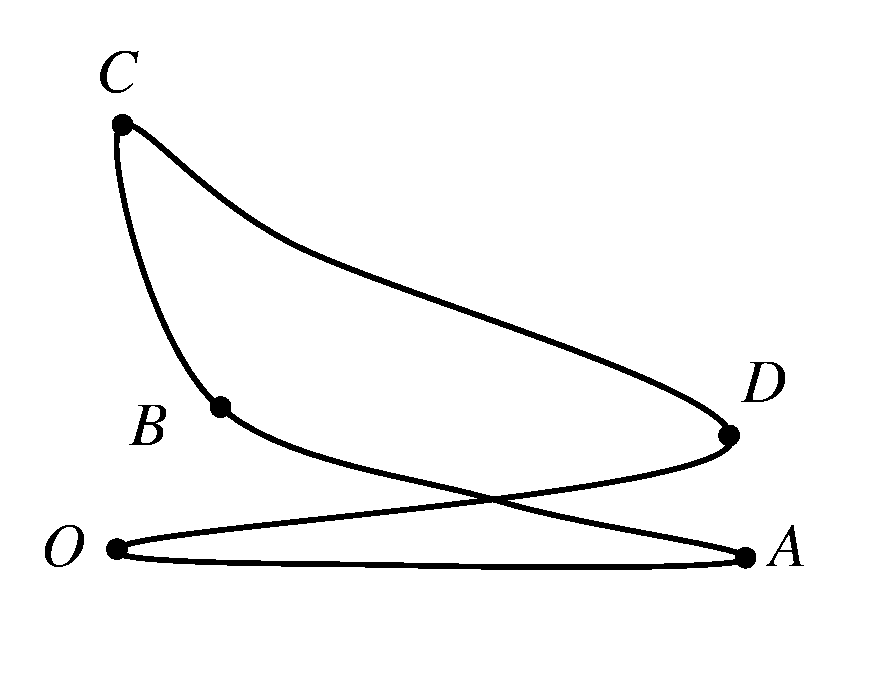
\includegraphics[width = \marginparwidth]{ciclo_8.pdf}
    \caption{Rappresentazione approssimativa del ciclo di Otto in
    condizioni reali. Sono evidenziate anche le coordinate teoriche
    corrispondenti a quelle presenti in figura \ref{erciclodiesel}.}
    \label{ciclo8}
\end{marginfigure}

Nella realtà, il ciclo Diesel come appena mostrato è ben lontano
da quelli che vengono solitamente progettati. In figura \ref{ciclo8}
viene mostrato il \textit{ciclo Otto}, molto simile a quello Diesel
e dal quale traggono ispirazione i maggiori tipi di motori termici
attuali. Si deve essere coscienti del fatto che la forma in figura
subisce numerosissime fluttuazioni sul piano $pV$ e l'intera trasformazione
è ovviamente irreversibile. Tutto ciò spiega il crollo drastico
dell'efficienza prevista teoricamente.

\subsubsection*{Un modo di cicli}
Abbiamo grattato solamente la superficie del mondo dei cicli termodinamici
impiegati come principi di funzionamento delle macchine.
Una delle prossime sezioni discute in dettaglio il ciclo di Carnot,
ma precisiamo che ne esistono molti altri\footnote{\href{https://it.wikipedia.org/wiki/Macchina_termica\#Esempi}{\textcolor{blue}{Wikipedia - Macchina Termica, Esempi}}.} %occhio al backslash nell'url. Serve da escape per la gratella
che si aggiungono a quello di Diesel.




\section{Principio secondo}
Dopo aver introdotto il concetto di macchina e della sua efficienza,
è legittimo chiedersi se è possibile progettare nella realtà
la macchina perfetta, che cioè converte tutta l'energia
(in particolare calore) in ingresso interamente in lavoro in uscita,
con efficienza unaria (100\%).
Operando ciclicamente, per una macchina dovrebbe seguire dal primo
principio $\Delta U = Q - W$ la conclusione $\Delta U = 0$ e allora

\[ Q = W \]

\noindent La teoria sembrerebbe essere fondata: lavoro e calore sono
convertibili, cioè spendendo calore otteniamo lavoro e possiamo tra l'altro
invertire il processo, perché l'uguaglianza non ci impone un
verso preferenziale e noi siamo tanto furbi da costruire macchine
in grado di funzionare al contrario. Per esperienza, tuttavia, è evidente che non
è così, cioè se spendiamo una certa quantità di calore $Q$ e
la trasformiamo in lavoro, sembra impossibile, mediante quel lavoro,
riottenere tutto il calore $Q$ iniziale. Per fare un esempio, potremmo
immaginare di costruire un mulino ad acqua in questo modo: sappiamo che
tutti i mulini sono mossi dalla corrente e in tal modo producono
lavoro; potremmo dunque far sì che il mulino alimenti una pompa che
riporta l'acqua in cima al mulino, facendolo muovere indefinitamente.
Assumendo che il dispositivo sia costruito in maniera
eccellente, riducendo quanto possibile dispersione e attriti,
in realtà questa macchina è destinata a fermarsi dopo un certo
intervallo di tempo\footnote{Consigliamo di dare un'occhiata alla
sezione dedicata al moto perpetuo, negli approfondimenti di questo
capitolo.}, sia esso una manciata di secondi o qualche milione di
anni.

Potremmo ribattere affermando che la realtà ci pone problemi come
attrito e dissipazioni di vario genere. Ciò che è sconcertante è
l'impossibilità non solo reale di costruire macchine simili,
ma anche teorica. Questa conclusione, come vedremo, fonda
le radici nel secondo principio, che a sua volta poggia sulla
seguente evidenza:

\begin{center}
    \textit{il calore non fluisce \underline{\emph{mai spontaneamente}} da un corpo ad uno più caldo}.
\end{center}

\noindent Con questo possiamo spiegare perché le macchine frigorifere
funzionano in un verso innaturale: remano contro questo fatto di natura,
permettendo al calore di fluire \emph{non spontaneamente} da sorgenti
fredde a sorgenti calde.

\subsection{Enunciati}
Esistono due enunciati celebri del secondo principio della termodinamica\footnote{Anche se storicamente non fu così, trattiamo prima l'attuale forma
del secondo principio della termodinamica, permettendoci di chiarire
le sezioni successive.}.
In qualità di principi, essi sono dati per veri sulla base dell'esperienza,
ma è comunque possibile dimostrare che essi si riferiscono alla
stessa proprietà della natura.

\begin{tcolorbox}[colback = red!30, colframe = red!30!black, title = {Enunciati del secondo principio della termodinamica}]
    \begin{itemize}
        \item \textbf{Enunciato di Kelvin-Plank}
        
        \begin{center}
            \textit{È impossibile realizzare una macchina il cui unico risultato
            sia quello di trasformare calore, a partire da una sola sorgente, interamente in lavoro.}
        \end{center}
    
        \item \textbf{Enunciato di Clausius}
        
        \begin{center}
            \textit{È impossibile realizzare un processo il cui unico risultato\\
            sia quello di trasferire calore da un corpo ad uno più caldo.}
        \end{center}
    \end{itemize}
\end{tcolorbox}

\noindent Una delle proprietà della natura che il secondo principio sottointende
è il fatto che ogni macchina termica, qualsiasi essa sia (anche tra quelle non ancora
inventate!) deve sempre operare tra almeno due sorgenti affiché essa possa
funzionare. Inoltre, da come si evince dall'enunciato di Kelvin-Plank, è impossibile
costruire macchine con rendimento pari a 1.

\subsection{Equivalenza degli enunciati}
Dimostreremo che i due enunciati sono equivalenti nel seguente modo:
indicando con $KP$ l'enunciato di Kelvin-Plank e con $C$ quello di
Clausius, concluderemo che $KP \Leftrightarrow C$ mostrando che
$\overline{KP} \Leftrightarrow \overline{C}$, cioè negando l'uno necessariamente
si deve negare anche l'altro\footnote{Dimostrazione: siano $a,b$ affermazioni
tali che $a \Leftrightarrow b$. Allora $(a \Leftrightarrow b) \equiv (a \Rightarrow b
\wedge b \Rightarrow a) \equiv (\lnot b \Rightarrow \lnot a \land \lnot a \Rightarrow \lnot b) \equiv (\lnot a \Leftrightarrow \lnot b)$,
dove nel terzo passaggio abbiamo impiegato la contronominale dell'implicazione $\Rightarrow$,
per cui $(x \Rightarrow y) \equiv (\lnot x \lor y) \equiv (\lnot\lnot\lnot x \lor \lnot\lnot y) \equiv (\lnot y \Rightarrow \lnot x)$.}. Di volta in volta
considereremo macchine che disobbediscono ai due principi, che chiameremo
sempre $\overline{KP}$ e $\overline{C}$, e che operano tra due
serbatoi 1 e 2 a temperature $T_1 < T_2$.

\subsubsection*{Dimostrazione: $\overline{KP} \Rightarrow \overline{C}$}
Cominciamo mostrando che $\overline{KP} \Rightarrow \overline{C}$,
facendo riferimento alla figura \ref{kptocproof}.
Consideriamo allora la macchina $\overline{KP}$ che preleva una
certa quantità di calore $Q_1 > 0$ da 1 e lo converte interamente
in lavoro $W$, alla facciaccia di Kelvin e Plank.

\[ Q_1 = W \]

\begin{marginfigure}
    \centering
    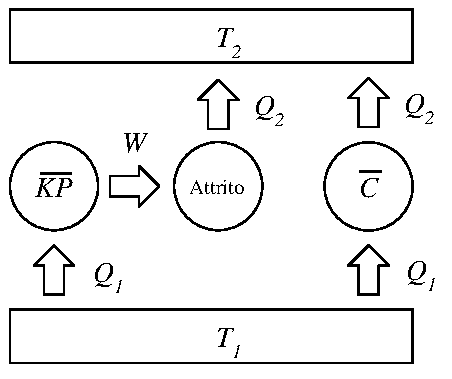
\includegraphics[width = \marginparwidth]{violare_kelvin-plank.pdf}
    \caption{Dimostrazione dell'implicazione $\overline{KP} \Rightarrow \overline{C}$.}
    \label{kptocproof}
\end{marginfigure}

\noindent Il lavoro $W$ viene poi impiegato per alimentare una
seconda macchina che cede il calore prodotto $Q_2$ alla sorgente
2. Questa macchina può essere progettata, per esempio, sulla base
di trasformazioni isoterme, oppure dissipando il lavoro meccanico
in attrito, che genera sempre calore. Allora

\[ Q_2 = -W \]

\noindent Ma allora,
se uniamo le macchine, ne otteniamo una che nel complesso preleva
del calore $Q_1$ dalla sorgente fredda 1 e cede quella stessa
quantità di calore alla sorgente calda 2, senza produrre altri
risultati. Questa macchina composta è proprio $\overline{C}$.

\begin{marginfigure}
    \centering
    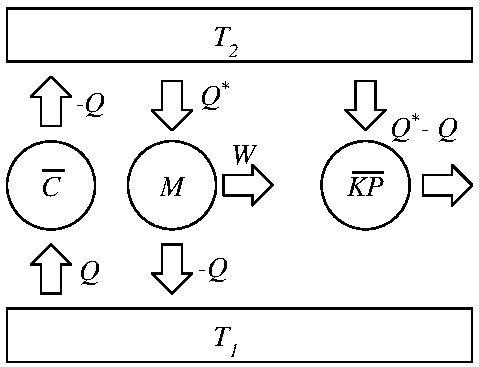
\includegraphics[width = \marginparwidth]{violare_clausius.pdf}
    \caption{Dimostrazione dell'implicazione $\overline{C} \Rightarrow \overline{KP}$.}
    \label{ctokpproof}
\end{marginfigure}

\subsubsection*{Dimostrazione: $\overline{C} \Rightarrow \overline{KP}$}
Si osservi la figura \ref{ctokpproof}.
Supponiamo di avere una macchina $\overline{C}$ che trasferisce
calore $Q > 0$ da 1 verso 2. Il calore in entrata nella macchina è
$Q_1 = Q$ mentre quello in uscita è $Q_2 = -Q$.
Consideriamo poi una seconda macchina $M$, progettata per prelevare
del calore $Q^* > Q$ dalla sorgente calda 2, produrre lavoro $W$
e cedere calore $Q_c = -Q$ alla sorgente fredda 1. Questo è ammissibile
operando sul rendimento $\eta_M = 1 - |Q_c|/Q^*$ di $M$.
Se si uniscono $\overline{C}$ e $M$, si ottiene una macchina che nel
complesso assorbe calore $Q^* - Q$ dalla sorgente calda 2, produce
lavoro $W$ ma che preleva per poi cedere di nuovo lo stesso calore
$Q$ alla sorgente 1, come se non esistesse. Dunque $W = Q^* - Q$.
La macchina composta corrisponde allora a $\overline{KP}$.

Si potrebbe ribattere sostenendo che $\overline{KP}$ può funzionare
perché vi è comunque scambio di calore $Q$ con la sorgente fredda,
anche se questo calore viene sempre ceduto e prelevato ripetutamente,
ma comunque questo ragionamento non regge. Per convincerci di ciò,
basta pensare ad un'altra macchina composta $X$ che incorpora
$\overline{KP}$ (costruita precedentemente) e la sorgente 1, mentre la 2
rimane esterna. Non vediamo la sorgente 1, in quanto componente
della macchina $X$ che opera solamente con la sorgente 2. Allora anche $X$
è analoga ad una macchina di tipo $\overline{KP}$.


\section{Esperienza di Carnot}
Nel 1824, l'ingegnere francese Sadi Carnot pubblicò il
\textit{Réflexions sur la puissance motrice du feu et sur les machines
propres à développer cette puissance}. Trascurando il titolo
altisonante, la questione che egli affrontò nell'opera
scaturì dalla nascente competizione alimentata dalla rivoluzione industriale:
In quali condizioni una macchina termica ha il redimento
massimo, indipendentemente da come essa viene costruita? Come
vedremo, la potenza di questa domanda (e della sua risposta) sta
proprio nell'indipendenza dalla tecnologia con la quale la
macchina funziona. Non importa se essa è il motore di una monoposto
di Formula 1, lo scramjet del Boeing X-43 o un altro metodo di
propulsione di qualche civiltà aliena a noi sconosciuta.

\begin{marginfigure}
    \centering
    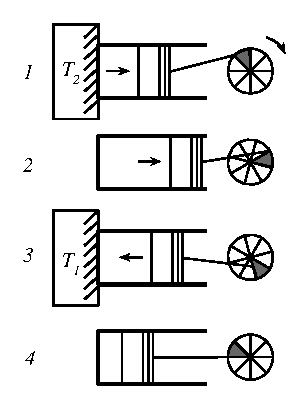
\includegraphics[width = \marginparwidth]{macchina_di_carnot.pdf}
    \caption{I quattro tempi che costituiscono il ciclo di funzionamento della macchina di Carnot.
    Il diagramma originale di Carnot non lo prevedeva, ma possiamo immaginare questa macchina come
    un classico motore che mette in rotazione un volano.}
    \label{macchinacarnot}
\end{marginfigure}

\subsection{Ciclo e macchina di Carnot}
Per rispondere ai suoi quesiti,
Carnot si ingegnò nella creazione di una macchina ideale,
la \textit{maccina di Carnot} (che indicheremo spesso con $\mathcal{C}$),
costituita da un cilindro che può esser reso adiabatico o
diatermico a piacere, un pistone mobile e un gas sottoposto al
\textit{ciclo di Carnot}. Altri componenti essenziali sono due
sorgenti a temperature differenti.
Un modello della macchina è mostrato in figura \ref{macchinacarnot}.
Durante un ciclo
di funzionamento, la macchina esegue i seguenti quattro passi
(consideriamo la sua versione termica, non frigorifera):


\begin{enumerate}
    \item \textit{Acquisizione di calore:} la macchina viene posta sulla
    sorgente calda. Supponendo che il gas sia già alla temperatura di
    questa sorgente, esso viene espanso isotermicamente, determinando
    il sollevamento del pistone e dunque la conversinoe di calore in
    lavoro.

    \item \textit{Raffreddamento adiabatico:} la macchina viene tolta dalla
    sorgente calda, ma il gas continua ad espandersi adiabaticamente
    (per questo il cilindro deve essere adiabatico durante questa
    fase) fino a raggiungere la temperatura della sorgente fredda.

    \item \textit{Cessione di calore:} il pistone viene abbassato per
    comprimere il gas, che isotermicamente cede calore alla sorgente
    fredda.

    \item \textit{Riscaldamento adiabatico:} la macchina viene tolta dalla sorgente
    fredda, ma il gas continua ad esser compresso adiabaticamente fino
    a raggiungere la temperatura della sorgente più calda. Il ciclo
    ricomincia.
\end{enumerate}

\begin{marginfigure}
    \begin{center}
        \begin{tikzpicture}
            \def\xmax{3}
            \def\ymax{2.5}
            \def\Th{1.20}
            \def\Tc{0.45}
            \def\Ch{0.4}
            \def\Cc{1.9}
            \def\N{40}
            \def\gam{2.2}
            \def\isotherm#1#2{{ #2/(#1) }}
            \def\adiabatic#1#2{{ #2/(#1)^(\gam) }}
            \def\xA{ (\Th/\Ch)^(1/(1-\gam)) }
            \def\xB{ (\Th/\Cc)^(1/(1-\gam)) }
            \def\xC{ (\Tc/\Cc)^(1/(1-\gam)) }
            \def\xD{ (\Tc/\Ch)^(1/(1-\gam)) }
            \coordinate (A) at ({\xA},{\isotherm{\xA}{\Th}});
            \coordinate (B) at ({\xB},{\isotherm{\xB}{\Th}});
            \coordinate (C) at ({\xC},{\isotherm{\xC}{\Tc}});
            \coordinate (D) at ({\xD},{\isotherm{\xD}{\Tc}});
            
            %\clip (-0.1*\xmax,-0.12*\ymax) rectangle (1.05*\xmax,1.1*\ymax);
            
            % WORK
            \fill[mylightblue,samples=\N]
                plot[domain={\xA:\xB}] (\x,\isotherm{\x}{\Th}) --
                plot[domain={\xB:\xC}] (\x,\adiabatic{\x}{\Cc}) --
                plot[domain={\xC:\xD}] (\x,\isotherm{\x}{\Tc}) --
                plot[domain={\xD:\xA}] (\x,\adiabatic{\x}{\Ch});
            \node[blue,scale=.9] at ($(B)!.5!(D)$) {$W$};
            
            % ADIABATIC & ISOTHERMIC TRANSFORMATIONS
            \draw[myred,thick,midarr=.60,domain={\xA:\xB},samples=\N]
                plot (\x,\isotherm{\x}{\Th}); % hot
            \draw[blue,thick,midarr=.45,domain={\xB:\xC},samples=\N]
                plot (\x,\adiabatic{\x}{\Cc}); % cold
            \draw[blue,thick,midarr=.65,domain={\xC:\xD},samples=\N]
                plot (\x,\isotherm{\x}{\Tc}); % cold
            \draw[myred,thick,midarr=.40,domain={\xD:\xA},samples=\N]
                plot(\x,\adiabatic{\x}{\Ch}); % hot
            
            % POINTS
            \fill[mydarkblue]
                (A) circle(0.05) node[above=1,scale=.8] {$A$}
                (B) circle(0.05) node[above right,scale=.8] {$B$}
                (C) circle(0.05) node[above=1,scale=.8] {$C$}
                (D) circle(0.05) node[below left,scale=.8] {$D$};
            
            % HEAT
            \draw[>={LaTeX[width=6,length=4]},->,line width=2,mydarkred]
                (.33*\xmax,.590*\ymax) --++ (-89:.56)
                node[pos=0,inner sep=0,anchor=-130,scale=.9] {$Q_\text{ass}$};
            \draw[>={LaTeX[width=6,length=4]},->,line width=2,mydarkblue]
                (.50*\xmax,.15*\ymax) --++ (-89:.56)
                node[inner sep=-2,anchor=60,scale=.9] {$Q_\text{ced}$};
            
            % AXIS
            \draw[->,thick] (0,-0.1*\ymax) -- (0,\ymax+0.1)
                node[anchor=north east,inner sep=4,scale=1] {$P$};
            \draw[->,thick] (-0.1*\xmax,0) -- (\xmax+0.1,0)
                node[anchor=north east,inner sep=4,scale=1] {$V$};
            
        \end{tikzpicture}
    \end{center}
    \caption{Il ciclo di Carnot sul piano $pV$.}
    \label{ciclodicarnot}
\end{marginfigure}


Carnot tiene a sottolineare come la macchina debba operare in condizioni
ben controllate, perché il gas al suo interno deve poter percorrere un
ciclo termodinamico \textit{quasistatico reversibile}. Perciò, lo spostamento
della macchina tra le due sorgenti, la compressione e l'espansione devono
essere estremamente lente, tanto da evitare attriti, dissipazioni di
calore, fluttuazioni irregolari nella temperatura,
turbolenze e comportamenti non ideali delle particelle del gas.
Una volta certi di aver soddisfatto questi requisiti, il
grafico del \textit{ciclo di Carnot} si presenterà nella forma mostrata
in figura \ref{ciclodicarnot}.

%\begin{marginfigure}
%    \centering
%    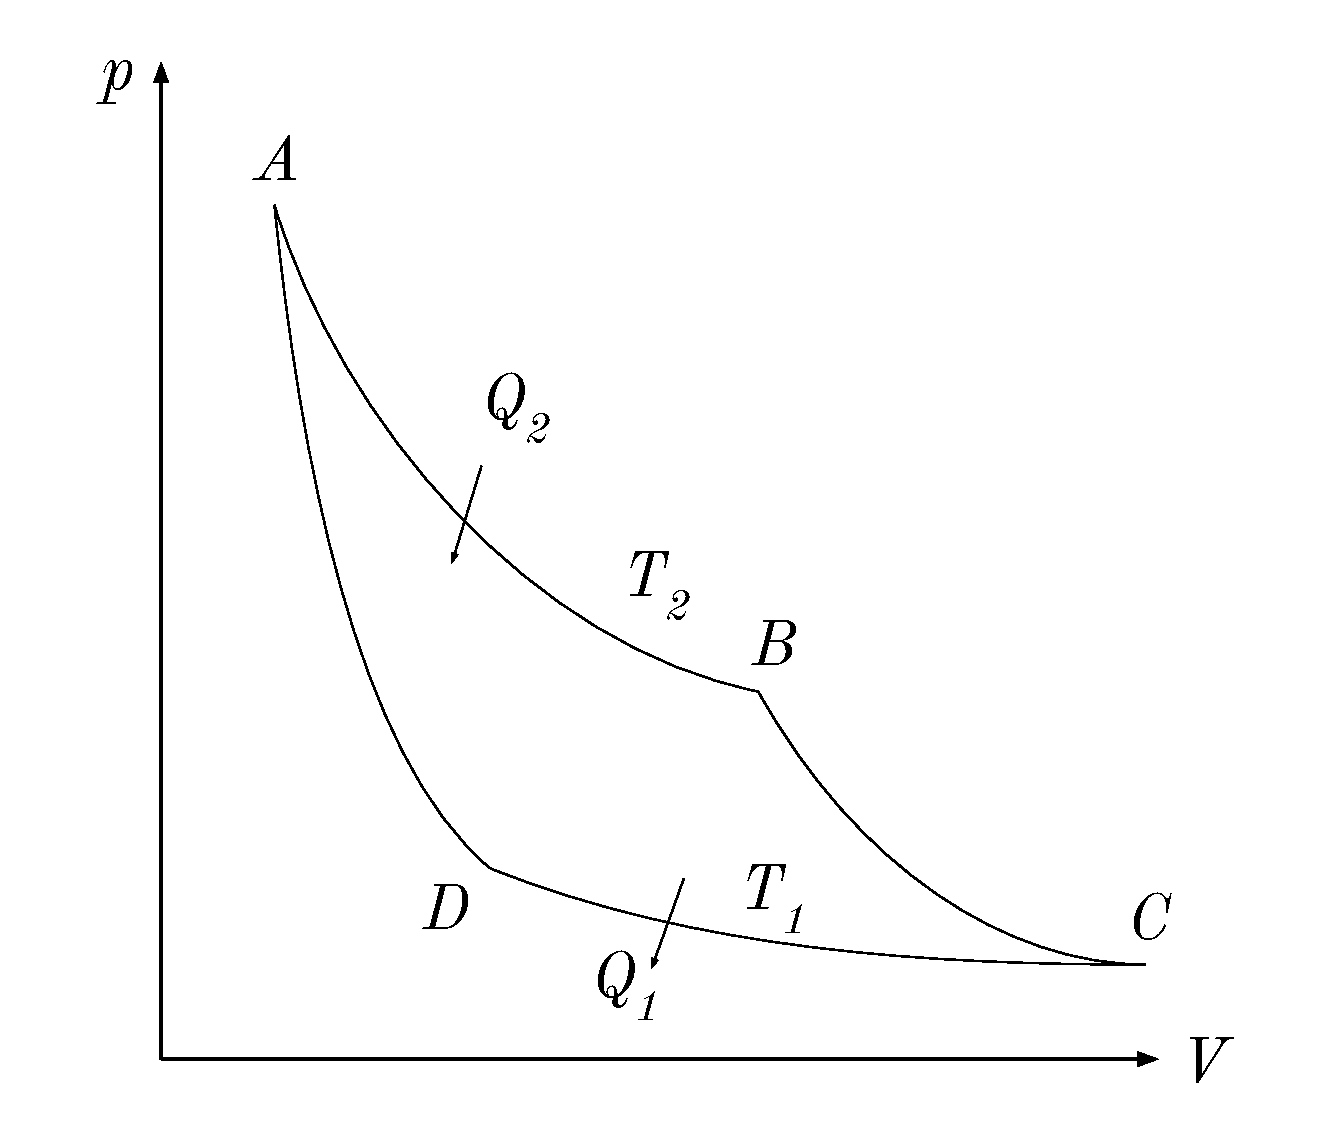
\includegraphics[width = \marginparwidth]{ciclo_di_carnot.pdf}
%    \caption{Il ciclo di Carnot sul piano $pV$.}
%    \label{ciclodicarnot}
%\end{marginfigure}



Analizzando il ciclo otterremo un risultato interessante.
Supponiamo che la sorgente fredda abbia temperatura $T_1$ mentre quella
calda $T_2$ e che la macchina di Carnot venga caricata di $n$ moli
di gas ideale. Calcoliamo gli scambi di energia nelle varie
trasformazioni che compongono il ciclo:

\begin{itemize}
    \item \textit{AB:} essendo una isoterma, $\Delta U_{AB} = 0$ e
    \[ Q_{AB} = W_{AB} = nRT_2\ln\left(\frac{V_B}{V_A}\right) > 0 \]
    Notare come questo costituisce il calore assorbito dalla macchina.

    \item \textit{BC:} essendo adiabatica, $Q_{BC} = 0$ e
    \[ \Delta U_{BC} = -W_{BC} = -nc_V(T_1 - T_2) \]

    \item \textit{CD:} la situazione è analoga a quella in \textit{AB}:
    \[ Q_{CD} = nRT_1\ln\left(\frac{V_D}{V_C}\right) < 0 \]

    \item \textit{DA:} come in \textit{BC}
    \[ \Delta U_{DA} = -W_{DA} = -nc_V(T_2 - T_1) \]
\end{itemize}

\noindent Abbiamo potuto usare le leggi ricavate dallo studio delle
trasformazioni elementari perché abbiamo supposto che il ciclo di
Carnot fosse quasistatico-reversibile. Veniamo ora alla risposta che
Carnot desiderava trovare: quale efficienza può essere raggiunta da
una tale macchina. Applicando la definizione di rendimento, dai
risultati precedenti è facile concludere che

\[ \eta_\mathcal{C} = \frac{W}{Q_{AB}} = 1 + \frac{T_1}{T_2}\frac{\ln(V_D/V_C)}{\ln(V_B/V_A)} \]

\noindent Ricordando la legge \ref{lativuu} che caratterizza le
trasformazioni adiabatiche, si scopre che l'efficienza qui sopra può
essere semplificata ulteriormente. Infatti, per la trasformazione
\textit{BC} vale $T_2V_B^{\gamma - 1} = T_1V_C^{\gamma - 1}$ mentre
per \textit{DA} $T_1V_D^{\gamma - 1} = T_2V_A^{\gamma - 1}$. Mediante
semplice algebretta, è evidente che $V_B/V_A = V_C/V_D$. Concludiamo
allora che

\begin{align}
    \eta_\mathcal{C} = 1 - \frac{T_1}{T_2}
\end{align}

Ecco dunque svelato l'arcano: idealmente, l'efficienza di una buona
macchina, ovvero ideale, dipende unicamente dalle temperature entro
le quali essa opera. Quanto più la loro differenza è grande, tanto
più la macchina sarà efficiente. Tuttavia, allo stato attuale della
nostra conoscenza della natura, non possiamo neppur teoricamente
ottenere $\eta_\mathcal{C} = 1$, (anzi $0 \leq \eta_\mathcal{C} < 1$),
perché dovremmo possedere un oggetto di temperatura $T_2 = +\infty$\footnote{Ammesso che ciò possa essere fisicamente sopportabile da qualche materiale misterioso, un corpo a temperatura infinita sarebbe
caratterizzato da un'energia interna infinita, il che minerebbe la
solidità dei principi di conservazione fin ora incontrati.},
oppure un oggetto a temperatura nulla\footnote{Si faccia
riferimento agli approfondimenti di questo capitolo per giustificazioni
alternative dell'impossibilità di raggiungere lo zero assoluto.}.

Vale inoltre per una macchina di questo tipo

\[ 1 - \frac{T_1}{T_2} = 1 - \frac{|Q_\text{ced}|}{Q_\text{ass}} \]

\noindent per cui

\begin{align}
    \frac{T_1}{T_2} = \frac{|Q_\text{ced}|}{Q_\text{ass}}
\end{align}



\subsection{Teorema di Carnot}
Carnot progettò mentalmente una macchina semplice ma inrealtà
particolare, che ha ben poco a che fare con il motore, ad esempio,
di una turbina di un aereo. Per questo motivo è stato formulato
il teorema di Carnot, con il quale si estende la valutazione
dell'efficienza a \textit{tutte} le macchine che operano tra due
sole sorgenti, anche quelle non ancora progettate.


\begin{tcolorbox}[colback = red!30, colframe = red!30!black, title = {Teorema di Carnot}]
Il rendimento di una qualsiasi macchina termica $X$ (reversibile o non)
che opera tra due
temperature costanti $T_1,T_2: T_1 < T_2$ è limitato superiormente dal rendimento della
macchina di Carnot $\mathcal{C}$ che lavora tra le medesime temperature.

\begin{align}
    \eta_X \leq \eta_\mathcal{C} \quad \text{per } T_1 < T_2\label{carnot1}
\end{align}

Inoltre, tutte le macchine reversibili che operano con la stessa coppia di temperature
hanno lo stesso rendimento, che equivale a quello della corrispondente macchina di
Carnot. Se $X$ è una macchina reversibile, allora:

\begin{align}
    \eta_X = \eta_\mathcal{C}\label{carnot2}
\end{align}

\end{tcolorbox}


\subsubsection*{Dimostrazione}
Si faccia riferimento alla figura \ref{teo_carnot}.
Per dimostrare il teorema, consideriamo una macchina $X$ qualsiasi
e una macchina di Carnot $\mathcal{C}$. Esse operano tra le solite
sorgenti a temperature $T_1$ e $T_2 > T_1$.
$X$ è costruita in tal guisa da produrre lavoro $W'$ e scambiare
calore $Q_1' < 0$ e $Q_2' > 0$ con le rispettive sorgenti. $\mathcal{C}$
produce invece $W$ e scambia $Q_1 < 0$ e $Q_2 > 0$.
Non sappiamo ancora nulla sui loro rendimenti né quale sia la migliore.
Quale dunque vincerà questa battaglia?
Chi scommette su $X$ sosterrà che

\[\eta_X \stackrel{?}{>} \eta_\mathcal{C} \]

\begin{marginfigure}
    \centering
    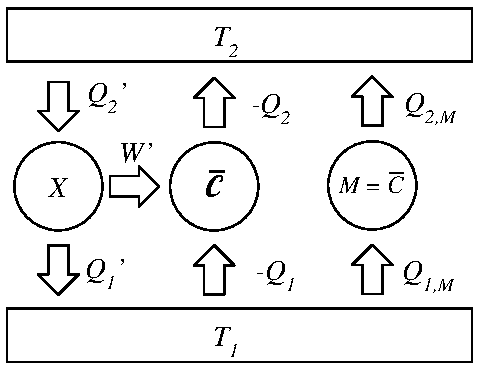
\includegraphics[width = \marginparwidth]{violare_carnot.pdf}
    \caption{Dimostrazione del primo enunciato del teorema di
    Carnot.}
    \label{teo_carnot}
\end{marginfigure}

La macchina di Carnot è per definizione reversibile. Esiste dunque
la sua versione frigorifera $\overline{\mathcal{C}}$ che opera al contrario.
$\overline{\mathcal{C}}$ avrà bisogno di lavoro esterno $-W$ per operare,
prelevando dalla sorgente fredda il calore $-Q_1$ e cedendo nel
complesso $-Q_2$ a quella calda. Immaginiamo che le due macchine
vengano ora accoppiate, in modo che $X$ alimenti $\overline{\mathcal{C}}$.
Ciò che ne deriva è una macchina $M$ che compie un certo lavoro
$W_M = W' - W$ e scambia certe quantità di energia con le sorgenti
tali che $Q_{1,M} = Q_1'-Q_1$ e $Q_{2,M} = Q_2' - Q_2$. $X$ è infine
progettata cosicché $W' = W$, cioè essa fornisce il lavoro di cui
$\overline{\mathcal{C}}$ ha bisogno. Ciò a cui vogliamo arrivare è
confrontare le efficienze a parità di lavoro prodotto.
Se allora si sostiene che $\eta_X > \eta_\mathcal{C}$ (attenzione che
ora torniamo a considerare $\mathcal{C}$! Possiamo farlo per supposizione
di reversibilità), ciò equivale
ad assumere che $W/Q_2' > W/Q_2$ da cui $Q_2 > Q_2'$. Come ci si
aspetterebbe, a parità di lavoro prodotto, $X$ consuma meno calore di
quello che invece utilizzerebbe $\mathcal{C}$.
Però in $M$ sta accadendo qualcosa che non dovrebbe: infatti
avremmo $Q_{2,M} < 0$, $W_M = 0$ e pertanto $Q_{1,M} > 0$. $M$ è proprio
una macchina che viola il secondo principio della
termodinamica secondo la formulazione di Clausius, perché non accade
altro che un trasferimento di calore dalla sorgente fredda a quella calda.
Purtroppo per chi ha puntato su $X$, si conclude che \[ \eta_X \leq \eta_\mathcal{C} \]

Se poi si assume che anche $X$ è reversibile, risulta che
$\eta_X \geq \eta_\mathcal{C}$ (basti ripercorrere la dimostrazione
sostituendo $X$ con $\mathcal{C}$), da cui si dimostra facilmente
che \[ \eta_X = \eta_\mathcal{C} \] Da questa conclusione, con
la quale termina la dimostrazione dell'intero teorema di Carnot,
si può osservare che la macchina di Carnot e tutte le macchine
reversibili che operano tra le stesse temperature sono equivalenti
in termini di efficienza; pertanto, la dimostrazione potrebbe essere
ripetuta anche senza limitarsi alla specifica macchina di Carnot,
eliminando, come proprio voleva Carnot, le particolari ``implementazioni''
che potrebbero rendere una macchina diversa dall'altra.

Nel caso $X$ non fosse reversibile, ciò significherebbe che
nessuna macchina reversibile può raggiungere, né tantomeno
superare, l'efficienza della corrispondente macchina di Carnot
che opera tra le medesime sorgenti. Non importa la macchina,
le sue prestazioni energetiche saranno sempre limitate superiormente
secondo l'espressione $1 - T_1/T_2$.

\subsection{Osservazioni di Carnot}
Da Carnot è possibile osservare che, se $Q_1 < 0$ è il calore ceduto
alla sorgente fredda e $Q_2 > 0$ quello assorbito dalla sorgente
calda, per le definizioni alternative di rendimento vale

\[ 1 + \frac{Q_1}{Q_2} \leq 1 - \frac{T_1}{T_2} \]

\noindent Che ci porta a concludere con la seguente:

\begin{align}
    \frac{Q_1}{T_1} + \frac{Q_2}{T_2} \leq 0
\end{align}

\noindent Ovviamente l'uguaglianza vale solo per macchine reversibili.
A prima vista, questa disuguaglianza potrebbe non comunicare
alcunché di straordinario. Nei prossimi paragrafi vedremo che
proprio da questa innocua relazione trarremo l'osservazione
forse più inquietante ma allo stesso tempo affascinante di
questo corso.

Un'altra osservazione: la seconda proposizione del teorema di Carnot
è molto importante, perché ci assicura, almeno sul piano teorico, che
le leggi della termodinamica valgono indipendentemente da come costruiamo
la nostra macchina, anche se questa non esiste ancora!

\section{Esperienza di Clausius}
Un ulteriore personaggio degno del titolo di \textit{main character}
della termodinamica è il tedesco Rudolf Clausius, il quale estese
gli studi di Carnot. Di fatto, il teorema di Carnot non è sufficientemente
generale, è ancora distante dalla nostra realtà, perché nelle trasformazioni
Carnot impone la presenza di due sole sorgenti distinte. Illustriamo nel seguito
il teorema di Clausius, che apre la strada ad uno degli ultimi concetti di questi
appunti: l'entropia.

\subsection{Teorema di Clausius}
Abbiamo visto che una delle relazioni ottenute da Carnot è la
somma di rapporti $Q_1/T_1 + Q_2/T_2 \leq 0$. Ciò vale per tutte
le macchine, reversibili o meno, che operano tra due sorgenti 1
e 2 tali che $T_1 < T_2$. Avere però solamente due sorgenti è
alquanto limitante e irrealistico, perché nella realtà le macchine
operano su cicli ben più complessi, fluttuando tra svariati valori
di temperatura, come se operassero tra infinite sorgenti. Clausius
ebbe così la brillante idea di generalizzare le conclusioni di
Carnot per un ciclo termodinamico qualsiasi.

Si consideri il ciclo motore mostrato in figura. Esso attraversa
un infinità di temperature differenti. Immaginiamo di approssimare
la curva di questo ciclo mediante piccole trasformazioni adiabatiche
e isoterme. Se estendiamo queste piccole trasformazioni, otterremo
una griglia che suddivide l'area interna del nostro ciclo in tanti
piccoli cicli di Carnot. Per il ciclo $i$-esimo, vale allora
$Q_{1,i}/T_{1,i} + Q_{2,i}/T_{2,i} \leq 0$. Sommando i rapporti di
tutti i cicli otteniamo

\[ \sum_i \left(\frac{Q_{1,i}}{T_{1,i}} + \frac{Q_{2,i}}{T_{2,i}}\right) \leq 0 \]

\noindent Questa relazione non ci dice ancora molto di straordinario,
anche se possiamo notare due fatti: i tratti adiabatici non coinvolgono
scambi di calore per definizione e dunque possiamo ignorarli nel
nostro calcolo, perché il rapporto calore-temperatura è sempre nullo
durante questo tipo di trasformazione; esistono poi molti tratti
isotermi che vengono percorsi in versi opposti da cicli adiacenti.
Ciò accade nei tratti interni alla curva originale e non introducono
contributi calorici. Gli unici tratti di nostro interesse sono
quelli delle trasformazioni isoterme ai bordi del ciclo. Possiamo
allora riformulare la somma unendo solamente i rapporti di questi
tratti. Supponendo che il tratto $j$-esimo sia una isoterma che
costituisce parte del bordo della curva originale, vale
$\sum_j Q_j/T_j \leq 0$. Più elegantemente, passando all'infinitesimo
si ottiene la seguente disuguaglianza

\begin{align}
    \oint \frac{dQ}{T} \leq 0\label{intclausius}
\end{align}

\noindent che è proprio la tesi del teorema di Clausius. L'integrale
che compare al membro sinistro della relazione \ref{intclausius}
prende il nome di integrale di Clausius. Il caso particolare
dell'uguaglianza vale solamente per trasformazioni reversibili.

\subsection{Conseguenze del teorema di Clausius}
L'integrale di Clausius da solo non comunica alcunché di interessante.
Se però lo consideriamo nel caso in cui il teorema \ref{intclausius}
vale per macchine reversibili, allora l'integrale è uguale a 0. Quando
zeri e integrali compaiono insieme in una relazione, spesso si
nasconde una qualche proprietà mistica.

Si consideri una trasformazione termodinamica \textit{reversibile} qualsiasi.
Per ipotesi di reversibilità, l'integrale di Clausius calcolato sulla curva $\tau$
di tale trasformazione nel piano pressione-volume è nullo.

\[ \oint_\tau \frac{dQ}{T} = 0 \]

\noindent Selezioniamo due punti, $A$ e $B$, distinti su questo ciclo. Scomponiamo
dunque l'integrale nei due percorsi, sempre reversibili, $\alpha$ e $\beta$.

\[ \int_{A,\alpha}^{B} \frac{dQ}{T} + \int_{B,\beta}^{A} \frac{dQ}{T} = 0 \]

\noindent Trattandosi di un ciclo reversibile, vale la proprietà antisimmetrica
dell'integrale. Giungiamo dunque alla seguente conclusione:

\[ \int_{A,\alpha}^{B} \frac{dQ}{T} = \int_{A,\beta}^{B} \frac{dQ}{T} \]

\noindent Questo significa che, passando dallo stato $A$ allo stato
$B$, non ha alcuna importanza se il percorso scelto è $\alpha$, $\beta$
o una qualsiasi altra trasformazione (reversibile!). L'integrale
$\int_{A}^{B}dQ/T$ ha lo stesso valore in tutti i casi, purché i
passaggi siano reversibili. Come per l'energia potenziale,
abbiamo trovato una quantità che non dipende dal percorso che
scegliamo per calcolarla, ma è legata solamente dagli stati
iniziali e finali. Questa proprietà di stato si chiama entropia.

\section{Entropia}
Siamo di fronte all'ultima creatura leggendaria di questo corso,
l'entropia, che approfondiamo in questa sezione dopo averla introdotta
come conseguenza degli studi di Clausius.

\subsection{Variazione di entropia}
A partire dal teorema di Clausius, definiamo la differenza di entropia
tra due stati termodinamici.

\begin{align}
    \Delta S_{AB} \stackrel{\text{def}}{=} \int_{A,\text{rev}}^{B} \frac{dQ}{T}\label{variaz_entropia}
\end{align}

L'entropia è una funzione di stato, come abbiamo
potuto vedere nei paragrafi precedenti. Da un punto di vista dimensionale, l'entropia
è un semplice rapporto tra energia e temperatura, una sorta di
indice della quantità di calore scambiato ad una data temperatura.
Durante gli scambi energetici, però, spesso la temperatura dei corpi
coinvolti cambia. Possiamo approssimare queste trasformazioni immaginando
infinitesimi quanità di calore che vengono scambiate di volta in volta
a temperature diverse. La variazione infinitesima di entropia corrisponde
allora al rapporto

\begin{align}
    dS \eqdef \left[\frac{dQ}{T}\right]_\text{reversibile}\label{entropia_infinitesima}
\end{align}

\subsubsection*{Cos'è l'entropia?}
Facciamo presente che in questo corso definiamo solamente la variazione
di entropia, non l'entropia assoluta di un sistema, un po' come si fa
con l'energia potenziale. Però, rispetto a quest'ultima, l'entropia
può essere definita (si vedano gli approfondimenti per brevi accenni,
in particolare la definizione \ref{entropia_meccanica_statistica}) ma
per i nostri scopi non è molto utile. Ancora non possiamo rispondere
con più profnodità alla domanda ``cos'è l'entropia?'' perché per
rispondere vogliamo fornire un quadro completo dell'entropia tramite
un ultimo teorema.


\subsection{Entropia nelle trasformazioni termodinamiche}
L'entropia può essere molto divertente quando applicata alle
trasformazioni termodinamiche, siano esse quelle fondamentali
oppure complesse.

\subsubsection{Entropia nelle trasformazioni fondamentali}
Possiamo aggiungere la variazione di entropia a tutte quelle equazioni viste nelle
trasformazioni termodinamiche fondamentali. Supponiamo come sempre
che tali trasformazioni siano quasistatiche reversibili. Applichiamo
le definizioni \ref{variaz_entropia} e \ref{entropia_infinitesima},
quindi per ogni trasformazione cerchiamo il calore $dQ$ e
la temperatura alla quale esso viene scambiato, riconducendoci
in alcuni casi a relazioni che legano il calore con la temperatura
stessa per ottenere funzioni da integrare, passando da $dS$ a $\Delta S$.

\begin{itemize}
    \item \textbf{Isoterma:} nelle isoterme abbiamo scoperto che
    $dQ = nRTdV/V$. Ci basta dividere questo calore per la temperatura
    alla quale sta avvenendo la trasformazione, ottenendo dunque
    
    \begin{align}
        dS_\text{isoterma} = nR\frac{dV}{V}
    \end{align}

    \noindent Integrando, otteniamo

    \begin{align}
        \Delta S_{AB} = nR\ln\left(\frac{V_B}{V_A}\right)
    \end{align}

    \noindent Possiamo notare che, in una isoterma, $\Delta S_{AB} > 0 \Leftrightarrow V_B > V_A$.
    Ciò è compatibile con l'intuizione dell'idea di entropia: se il gas
    si ``sparge'' in un volume maggiore, il suo disordine è maggiore e
    dunque aumenta la sua entropia.

    \item \textbf{Isocora:} dalla nostra tabellazza sappiamo che $dQ = nc_VdT$,
    quindi

    \begin{align}
        dS_\text{isocora} = nc_V\frac{dT}{T}
    \end{align}

    \noindent da cui

    \begin{align}
        \Delta S_{AB} = nc_V\ln\left(\frac{T_B}{T_A}\right)
    \end{align}

    \noindent In questo caso, $\Delta S_{AB} > 0 \Longleftrightarrow T_B > T_A$.
    Intuitivamente, il disordine del sistema aumenta per via dell'incremento
    di temperatura. Immaginando un gas ideale (ma anche un cubetto di ghiaccio
    in una tazza di té, the, htegh, o come si scrive), di fatto le particelle
    si agitano di più e il sistema diventa più caotico.

    \item \textbf{Isobara:} vale $dQ = nc_pdT$ e allora
    
    \begin{align}
        dS_\text{isobara} = nc_p\frac{dT}{T}
    \end{align}

    \noindent e allora

    \begin{align}
        \Delta S_{AB} = nc_p\ln\left(\frac{T_B}{T_A}\right)
    \end{align}

    \noindent La spiegazione intuitiva è pressoché la stessa di
    quelle precedenti. Anzi, da un certo punto di vista si tratta
    proprio di una combinazione delle prime due.

    \item \textbf{Adiabatica:} abbiamo $dQ = 0$.
    
    \begin{align}
        dS_\text{adiabatica} = 0
    \end{align}

    \noindent da cui ovviamente segue che $\Delta S_{AB} = 0$.
    In questa trasformazione la spiegazione intuitiva del
    binomio entropia-disordine è più complessa. Per andare al punto,
    immaginiamo una compressione adiabatica di un gas: il suo
    volume diminuisce, quindi saremmo tentati di concludere che
    l'entropia del sistema diminuisce, ma in realtà in una adiabatica
    deve aumentare anche lìenergia interna del gas, quindi anche la
    sua temperatura. Precedentemente abbiamo associato l'aumento di
    temperatura all'aumento di entropia. Perciò il disordine dovuto
    alla temperatura che si innalza compensa l'ordine che si introduce
    col volume. Il ragionamento è analogo per una decompressione
    adiabatica.
\end{itemize}

\noindent Aggiungiamo una formula bonus, la \textbf{variazione di
entropia in transizioni di fase}. Ricordiamo che, in un cambiamento
di fase (immaginiamo il ghiaccio che si scioglie, da solido a liquido),
bisogna fornire al sistema una certa quantità di calore proporzionale
alla massa che si intende trasformare. Questo è il calore latente,
che dipende da una costante $\lambda$. Allora possiamo scrivere
$dQ = \lambda dm$, ovvero una piccolissima quanità di calore che
permette ad una piccolissima quantità di massa di trasformarsi.
Concludiamo che

\begin{align}
    dS_\text{tfase} = \frac{\lambda dm}{T}
\end{align}

\noindent Ricordiamo anche che le transizioni di fase avvengono
(idealmente) a temperature costanti. Allora

\begin{align}
    \Delta S_{AB} = \frac{\lambda m}{T}
\end{align}

\subsubsection*{Diagramma temperatura-entropia}

\subsubsection*{Variazione di entropia in trasformazioni complesse}



\subsection{Il teorema dell'entropia}


\subsubsection{Che dire dei frigoriferi?}

% spiegaz di Iuppa differenza di entropia: calore sprecato in uno scampio, sprecato = non più recuperabile
\subsection{Disordine}
Uno dei tanti modi di vedere l'oggetto matematico dell'entropia
è quello del calore irrecuperabile.


\section{Approfondimenti}
Questo pacco di termodinamica si conclude, ma essendo grande
merita molti approfondimenti.

\subsection{La questione del calorico}
La fisica poggia su un substrato filosofico molto sofisticato e
sviluppato, dal quale hanno origine, per esempio, molte interpretazioni
della realtà che viene studiata. Una questione che segnò le ricerche
nel campo della termodinamica fu quella di definire e chiarire le
ragioni d'essere del \textit{calore}, ovviamente avanzando ipotesi
secondo il metodo scientifico.

Prima di Joule, si parlava in letteratura di \textit{calorico},
qualcosa che veniva interpretato come un fluido vero e proprio,
dotato di esistenza propria e in grado di muoversi da corpo a
corpo, da sorgenti più calde a quelle più fredde. La temperatura
veniva poi definita sulla base della concentrazione di calorico
in un certo corpo, anche se calore e temperatura rimanevano in
molti casi concetti confusi, come a volte capita anche nell'esperienza.

Grazie agli esperimenti di Joule, la fisica comprese che il calore
rappresenta in realtà una forma di energia, qualcosa che
non esiste in natura, ma che la descrive. Nell'esperimento del
mulinello, l'innalzamento di temperatura dell'acqua è dovuto al
lavoro compiuto da una massa in caduta. Secondo l'interpretazione
precedente, del calorico sarebbe comparso dal nulla, quando invece
viene semplicemente osservata una trasformazione di lavoro in calore,
in accordo con i principi di conservazione già sviluppati in meccanica.


\subsection{Espansione libera dei gas}
Mostriamo un semplice esperimento citato a lezione.


\subsection{Micro- e macro-stato}
Con i nostri strumenti non siamo in grado di definire l'entropia in
senso assoluto, ma solo la sua variazione. Studi più avanzati,
collegati alla cosiddetta \textit{meccanica statistica}, consentono
invece di esprimere in forma chiusa l'entropia di un sistema.

\begin{align}
    S \eqdef k_B \ln [N]\label{entropia_meccanica_statistica}
\end{align}

\noindent dove $k_B$ è la costante di Boltzmann, mentre $N$
corrisponde al \textit{numero di microstati compatibili con il
macrostato}. Vediamo cosa si intende con questa definizione,
mostrando un esempio molto celebre: supponiamo di avere due
scatole, $A$ e $B$, suddivise ciascuna in 6 scompartimenti
identici. In ogni scompartimento, o slot, può essere collocata
una sola pallina tra un mucchio di altre, identiche e indistinguibili
tra loro. La particolarità
di queste palline è la loro insolita abitudine di rimbalzare
da uno slot all'altro in maniera del tutto casuale ed imprevedibile.
Immaginiamo che la scatola $A$ contenga
un totale di 4 palline, mentre $B$ due. Se avviciniamo $A$ e
$B$, le palline cominceranno a saltare non solo negli slot
della stessa scatola ma anche in quelli dell'altra. La situazione è
mostrata in figura \ref{micromacro}. Il macrostato del sistema
costituito dalle due scatole $A$ e $B$ e dalle loro palline,
in totale 6, è descrivibile dalla proprietà \textit{numero di palline nella scatola $X$},
dove $X = A, B$. Per macroscopico intendiamo
il fatto di non essere per nulla interessati di dove si trovano
le palline in ciascuna scatola, ma solamente di conoscere il
loro numero totale, in $A$ o in $B$. Il microstato, invece,
è rappresentato dalla configurazione delle palline negli slot.

\begin{marginfigure}
    \begin{center}

        %STATO I
        \begin{minipage}{0.4\marginparwidth}
            \begin{center}
                $A(4)$
            \end{center}
            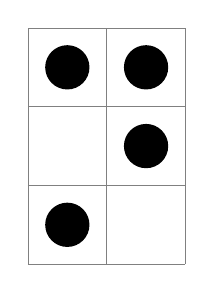
\begin{tikzpicture}
                %scacchiera
                \draw[step=1cm,gray,very thin] (0,0) grid (2,3);
                %cerchi dentro i quadrati
                \fill[black] (0.5,0.5) circle (8pt);
                \fill[black] (1.5,1.5) circle (8pt);
                \fill[black] (1.5,2.5) circle (8pt);
                \fill[black] (0.5,2.5) circle (8pt);
            \end{tikzpicture}
        \end{minipage}
        \begin{minipage}{0.4\marginparwidth}
            \begin{center}
                $B(2)$
            \end{center}
            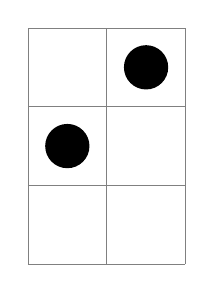
\begin{tikzpicture}
                \draw[step=1cm,gray,very thin] (0,0) grid (2,3);
                \fill[black] (0.5,1.5) circle (8pt);
                \fill[black] (1.5,2.5) circle (8pt);
            \end{tikzpicture}
        \end{minipage}

        \vspace{0.8cm}

        %STATO II
        \begin{minipage}{0.4\marginparwidth}
            \begin{center}
                $A(4)$
            \end{center}
            \begin{tikzpicture}
                \draw[step=1cm,gray,very thin] (0,0) grid (2,3);
                \draw[fill=none, draw=myblue, thick] (0.5,0.5) circle (8pt);
                \fill[black] (1.5,1.5) circle (8pt);
                \draw[fill=none, draw=myred, thick] (1.5,2.5) circle (8pt);
                \fill[black] (0.5,2.5) circle (8pt);

                %dischi mossi
                \fill[myblue] (1.5,0.5) circle (8pt);
            \end{tikzpicture}
        \end{minipage}
        \begin{minipage}{0.4\marginparwidth}
            \begin{center}
                $B(2)$
            \end{center}
            \begin{tikzpicture}
                \draw[step=1cm,gray,very thin] (0,0) grid (2,3);
                \fill[black] (0.5,1.5) circle (8pt);
                \draw[fill=none, draw=green, thick] (1.5,2.5) circle (8pt);

                \fill[myred] (0.5,2.5) circle (8pt);
                \fill[green] (0.5,0.5) circle (8pt);
            \end{tikzpicture}
        \end{minipage}
    \end{center}
    \caption{Rappresentazione dei microstati dell sistema di scatole
    $A$-$B$. In alto viene mostrata la situazione iniziale, in cui
    un particolare microstato determina il macrostato \textit{4 palline
    in $A$ e 2 in $B$}. In basso, il sistema passa ad un nuovo microstato,
    dove le palline che si sono mosse sono evidenziate con colori diversi
    (quelle vuote indicano la posizione precedente, quelle piene la nuova
    posizione).
    Notare che le palline possono muoversi anche tra le scatole; infatti,
    il macrostato diventa \textit{3 palline in $A$ e 3 in $B$}.}
    \label{micromacro}
\end{marginfigure}

%\begin{marginfigure}
%    \centering
%    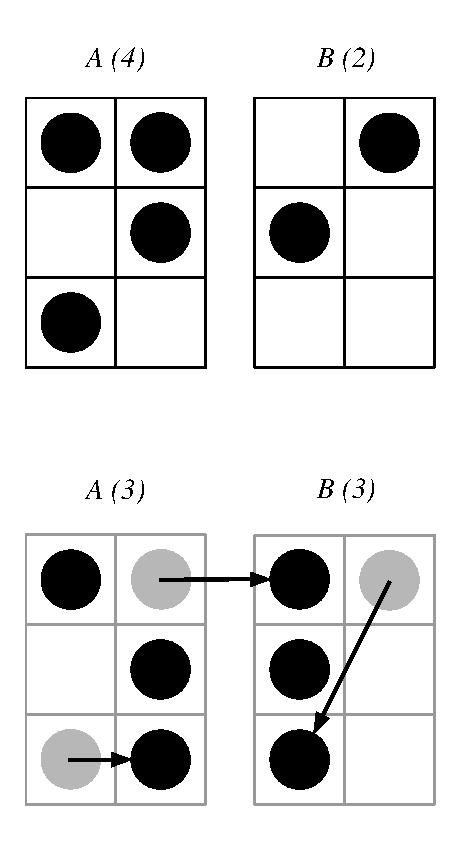
\includegraphics[width = \marginparwidth]{micro_macro_stati.pdf}
%    \caption{Rappresentazione dei microstati dell sistema di scatole
%    $A$-$B$. In alto viene mostrata la situazione iniziale, in cui
%    un particolare microstato determina il macrostato \textit{4 palline
%    in $A$ e 2 in $B$}. In basso, il sistema passa ad un nuovo microstato.
%    Notare che le palline possono muoversi anche tra le scatole; infatti,
%    il macrostato diventa \textit{3 palline in $A$ e 3 in $B$}.}
%    \label{micromacro}
%\end{marginfigure}

Poniamoci ora la domanda: quanti microstati sono compatibili
col macrostato \textit{4 palline in $A$, 2 in $B$}? Per rispondere,
ci basta applicare un pizzico di combinatoria\footnote{Ricorriamo
al metodo del coefficiente binomiale. Per ciascuna scatola, possiamo immaginare
di assegnare gli $n = 6$ slot alle $k$ palline del macrostato. Però, dal
momento che le palline sono tra loro indistinguibili, non dobbiamo incappare
nell'errore di contare configurazioni per le quali, scambiando due qualsiasi
palline, gli slot occupati sono sempre gli stessi. Il coefficiente binomiale
tiene conto di questo fatto senza contare eventuali configurazioni uguali,
ed è definito come $\binom{n}{k} = \frac{n!}{k!(n - k)!}$. Per finire, dato
che ci interessa conoscere le configurazioni totali del sistema scatola-$A$-scatola-$B$,
dobbiamo applicare il principio del calcolo combinatorio e moltiplicare tra
loro i coefficienti binomiali.},
determinando quante sono le configurazioni di 4 palline in 6 slot di $A$
e 2 in 6 slot di $B$. I microstati sono in tutto

\[ N_{4,2} = \binom{6}{4} \cdot \binom{6}{2} = 225 \]

Ora, poniamo vicine tra loro $A$ e $B$ e lasciamo che le palline
saltino tra l'una e l'altra scatola. Quante possibilità esistono
per cui vale il macrostato \textit{1 pallina in $A$, 5 in $B$}?
Ancora, la combinatoria ci fornisce il risultato

\[ N_{1,5} = \binom{6}{1} \cdot \binom{6}{5} = 36 \]

\noindent Notiamo immediatamente una cosa: il numero di microstati
compatibili è decisamente più piccolo. Proviamo a fare un ultimo
calcolo, contando invece i microstati per cui sono presenti
\textit{3 palline in $A$ e 3 in $B$}, ovvero le palline sono
equamente distribuite tra le due scatole:

\[ N_{3,3} =\binom{6}{3}^2 = 400 \]

In virtù della definizione \ref{entropia_meccanica_statistica}, possiamo concludere che
l'entropia del sistema con la configurazione 4-2, quella iniziale,
è minore di quella 3-3.
Dal momento che le palline si muovono tra gli slot in maniera
casuale, possiamo supporre che tutte le configurazioni possibili
siano equiprobabili, ma molte di esse, che sono singoli microstati,
corrispondono agli stessi macrostati. È dunque più probabile che
le palline si dispongano per lo più equamente tra $A$ e $B$
anziché disporsi tutte in una sola delle due, come i calcoli
rivelano. Se aumentiamo
le palline e gli slot, tra l'altro, il numero di microstati
vicini a quello in cui le palline sono esattamente divise
cresce esponenzialmente. Per la meccanica statistica, questo
è il motivo per cui i sistemi termodinamici tendono a massimizzare
la propria entropia. Ma questo non è dovuto al fatto che essi
``vogliono'' farlo, bensì perché è il destino più probabile.

Non abbiamo scelto l'analogia delle palline e delle scatole a caso.
Possiamo immaginare le palline come particelle di gas e le scatole
come contenitori dotati di volume, occupabile dalle particelle stesse
in svariate configurazioni. Oppure, le scatole possono essere
due barre di metallo, una calda e una fredda, e le palline
rappresentano i ``pacchetti'' di energia con i quali si può
quantificare il calore scambiato, oltre la temperatura delle barre durante
gli stati di equilibrio. Come già concluse Boltzmann, non è
del tutto vero che è impossibile che il gas si accatasti
tutto in un solo contenitore, oppure che il calore fluisca
dal corpo freddo a quello caldo. Nulla vieta il verificarsi di
certi fenomeni. Semplicemente, è estremamente
improbabile che ciò accada e questo vale ancor di più per sistemi
sempre più grandi e complessi, proprio quelli in cui viviamo noi.
Ricordate la famosa, apparentemente innocua osservazione scritta
all'inizio della sezione sul secondo principio? Ora dovrebbe essere
evidente l'importanza di quel \emph{mai spontaneamente}.

\subsubsection*{Entropia, disordine, informazione, tempo}
L'entropia non è propriamente qualcosa che esiste fisicamente,
ma è solo uno stratagemma matematico per mettere in luce una
certa regolarità del mondo.
Ma per noi umani, cos'è allora l'entropia? Alla luce di questa breve introduzione
alla meccanica statistica, non si tratta altro che una descrizione
del grado di disordine di un sistema: più i costituenti di un
sistema sono sparsi, disordinati, più l'entropia aumenta. Questo
è il motivo per cui il concetto di entropia trova svariati campi
d'applicazione al di fuori della fisica, tra le quali anche
l'informatica. Uno spunto interessante che ha permesso l'entropia
di avere successo in altre branche del sapere è il seguente: un
sistema disordinato richiede maggior informazione per essere
descritto rispetto ad uno ordinato, per via dei diversi gradi
di complessità che si possono presentare, come abbiamo visto
nell'esempio delle palline.

Come già emerge dal teorema dell'entropia, esiste una quantità
che varia in maniera differente a seconda del verso con cui il
tempo scorre. La nostra percezione del tempo è abituata a vedere
il succedersi degli eventi nella sequenza più naturale e spontanea
che esiste in natura, ovvero quella per cui i sistemi fisici tendono
a gradi di disordine sempre maggiori.

\subsection{Il terzo principio}
Ebbene sì: esiste un terzo principio della termodinamica che è stato
ignorato in queste lezioni. Esso introduce concetti già avanzati, ma,
in alcune delle sue formulazioni equivalenti, rimane comunque estremamente
affascinante. In breve, questo principio afferma che non esiste
temperatura più bassa dello zero assoluto e che quest'ultimo non è
neppur raggiungibile. Ecco una delle formulazioni:

\begin{center}
    \textit{Non esiste processo in grado portare la temperatura di un corpo\\allo
    zero assoluto tramite un numero finito di passi.}
\end{center}

\noindent Analogamente alle dimostrazioni viste per l'equivalenza
degli enunciati del secondo principio, anche il terzo può essere
dimostrato con un esperimento mentale che si basa sullo stesso principio
di funzionamento del frigorifero:

Supponiamo di avere un insieme di oggetti a 0 K e un oggetto $X$ da
raffreddare e a temperatura superiore. Mettiamo $X$ in
contatto termico con uno degli oggetti a 0 K. Sappiamo dalla calorimetria
che i due corpi raggiungeranno l'equilibrio termico e avranno una
temperatura uguale intermedia alle loro iniziali. Possiamo allora
ripetere il raffreddamento con $X$ e un altro oggetto a 0 K, ma
non raggiungeremo mai lo zero assoluto con un numero finito di
contatti, perché l'equilibrio termico viene raggiunto ad una temperatura
che è sempre compresa tra 0 K (escluso) e quella di $X$ raffreddato, che
è maggiore di 0 K.

Purtroppo per noi, non è ancora stato trovato un oggetto a 0 K\footnote{Sono
molti gli oggetti leggendari come questo in fisica: la massa infinita, il
corpo nero, il piano privo di attrito...}, né tantomeno sono state
trovate tecniche di raffreddamento in grado di raggiungere lo zero
assoluto, anche se siamo stati in grado di avvicinarci ad esso
nell'ordine di una frazione di Kelvin.


\subsection{Macchine e moto perpetuo}
Parlando di principio secondo, abbiamo ipotizzato l'esistenza di macchine
in grado di convertire l'energia fornita (il calore) in lavoro senza alcuna
dissipazione o perdita. Per via del secondo principio questo non è possibile
e ci siamo rassegnati presto ad esso. Ora che però siamo nella sezione approfondimenti,
possiamo fantasticare quanto ci pare: e se non valesse il secondo principio
della termodinamica? Per il primo principio, sarebbero ammesse le leggendarie
macchine super efficienti, che una volta azionate entrerebbero in un regime
di funzionamento conosciuto come moto perpetuo.

Una macchina capace di moto
perpetuo è in grado di produrre lavoro senza alcun apporto di energia esterno,
eccetto quello necessario ad azionarla. Ricordando sempre il caro, vecchio primo
principio, $\Delta U = Q - W$, sappiamo che $\Delta U = 0$ per via del
funzionamento ciclico delle macchine, da cui $W = Q$. $Q$ rappresenta l'energia
iniziale che innesca il moto, mentre $W$ è il lavoro prodotto. Attenzione però,
perché anche il primo principio pone un limite a queste macchine.
Dal momento che calore e lavoro si equivalgono, il moto perpetuo dovrebbe
convertire queste due forme di energia in continuazione. In altre parole,
la macchina può solo autoalimentarsi e non potremo mai sfruttarla per generare
energia infinita, pena lo spegnimento della macchina stessa.

Nella storia (anche in tempi recenti) sono state numerose le proposte
di macchine del genere, ma ovviamente nessuna di esse funziona.
Sottolineamo che il fantomatico moto perpetuo, \emph{prima o poi}, è
destinato a fermarsi. Non viene specificato dopo quanto tempo, che tuttavia
è sicuramente finito: una frazione infinitesima di secondo, un minuto,
un'ora, un anno, una decina di miliardi di anni.
Ecco alcuni esempi fantasiosi di moto perpetuo:

\begin{itemize}
    \item Il mulino: un mulino ad acqua aziona una pompa idraulica,
    che riporta il liquido in cima alla ruota, che quindi gira e
    produce lavoro per mantenere l'acqua in circolo e far ruotare
    sé stessa indefinitamente.

    \item La lampadina: una lampadina emette la stessa luce necessaria
    ad attivare dei pannelli fotovoltaici che la alimentano.

    \item Contenitore di Boyle: un vaso riempito di acqua possiede
    un tubo che dal fondo convoglia l'acqua in cima al contenitore.
    Il tubo è estremamente stretto e allungato mano a mano che si
    raggiunge l'estremità. Questa macchina idraulica dovrebbe permettere
    all'acqua di scorrere all'infinito nel tubo, ritornando nel
    vaso come una fontanella, perché per capillarità (per questo il tubo deve esssere molto
    stretto) il liquido dovrebbe essere risucchiato. Per svariate
    qestioni di pressione e fluidodinamica, la fontanella non
    riuscirà mai a scorrere.
\end{itemize}

Questi esempi mostrano che i principi della termodinamica non
sono validi solamente in quei sistemi in cui si trattano caldo,
freddo e così via. Come Carnot previde, le leggi reggono anche
per macchine costruite nelle maniere più bizzarre.

%\setcounter{chapter}{0}

\part{Appendici}
\appendix
\renewcommand{\thechapter}{\Alph{chapter}}
\chptr{Esercizi}

\section{Effetto centrifuga}

Un corpo è vincolato a muoversi lungo una guida
rigida (può muoversi parallelamente alla guida
ma non perpendicolarmente ad essa) che sta
ruotando intorno ad uno dei suoi estremi con
velocità angolare $\omega$ (rad/s). Inizialmente
il corpo si trova a $d_0$ m dall'asse di rotazione
ed è fermo; dopo un certo intervallo di tempo
il corpo ha raggiunto una posizione $d_f$ (m)
ed ha una velocità $v_f$ (m/s). Dati
$d_0 = 1$, $d_f = 2.5$, $v_f = 8.1$, trovare
$\omega$.
\begin{enumerate}
    \item 5.0
    \item 5.6
    \item 8.9
    \item 3.5
\end{enumerate}

\noindent \textbf{Soluzione:}
Fissiamo un sistema di riferimento
solidale con la guida. In tal modo, è come se
l'oggetto si stesse muovendo solamente in linea
retta sulla guida stessa. In tale situazione,
l'oggetto si sposta verso l'esterno per via
della forza centrifuga, una forza apparente,
perché il sistema di riferimento scelto
non è inerziale.

Ricorriamo ad una analisi energetica. L'energia
cinetica dell'oggetto viene incrementata dall'azione
della forza centrifuga; ciò suggerisce il ricorso
al teorema dell'energia cinetica:

\begin{align}
    \Delta E_K &= W_{F_c}\label{g1}\\
    K_f - K_0 &= \int_{d_0}^{d_f}F_c ds\label{g2}\\
    \frac12 m v_f^2 &= \int_{d_0}^{d_f}m\omega^2sds\label{g3}\\
    v_f^2 &= \omega^2(d_f^2 - d_0^2)\label{g4}
\end{align}

\noindent da cui il risultato cercato

\[ \omega = \frac{v_f}{\sqrt{d_f^2 - d_0^2}} \]

\noindent Eseguendo i calcoli, risulta che la risposta
(4) è quella corretta. Analizziamo più chiaramente i passaggi:
In \ref{g1} esprimiamo il teorema delle forze vive
come variazione dell'energia cinetica dell'oggetto
equivalente al lavoro compiuto dalla forza centrifuga $F_c$.
In \ref{g2} esplicitiamo la differenza tra le energie
cinetiche iniziale e finale; dall'altro membro costruiamo
invece l'integrale che permette di ottenere il lavoro
totale dalla posizione iniziale $d_0$ a $d_f$: ricorriamo
alla definizione più generale di lavoro (appunto impiegando
il calcolo integrale), perché $F_c$ varia durante il
percorso da $d_0$ a $d_f$. In \ref{g3} possiamo accorgerci
che l'energia cinetica iniziale è nulla (il testo afferma
che l'oggetto è inizialmente fermo rispetto alla guida);
al membro di destra esprimiamo invece $F_c$ in funzione
di $m$, $\omega$ e $s$, dove $s$ rappresenta la posizione
dell'oggetto a partire dal fulcro sul quale ruota la guida.
Per ricavare questa relazione
abbiamo utilizzato la definizione di forza centripeta
(che si rivela essere, in modulo, la stessa di quella
centrifuga)

\[ a_c = \omega^2 s \]

\noindent In \ref{g4} cancelliamo i termini comuni
come la massa e il fattore $\frac12$ (che compare
anche al membro di destra per via dell'integrazione
del tipo $\int xdx = x^2/2$). Notiamo poi che $\omega$
è costante, perché la guida ruota con velocità angolare
costante, e può essere ``estratto'' dall'integrale.


\section{Rincorsa sul cuneo}
Una massa $m$ (kg) si muove inizialmente su un piano
orizzontale privo di attrito con velocità $v_0$ (m/s).
Successivamente essa sale su un piano inclinato, inizialmente
fermo rispetto al piano orizzontale, di
massa $M$ (kg), che consiste in un cuneo libero di
muoversi anch'esso sul piano. La velocità $v_0$ è
tale che $m$ si ferma esattamente sulla sommità del
cuneo, ad altezza $h$ (cm). Si supponga che non vi
siano attriti di alcun genere. Dati $m = 11.0$, $M = 47.0$
e $h = 25.0$, trovare $v_0$.

\begin{enumerate}
    \item 4.1
    \item 8.5
    \item 2.5
    \item 6.0
\end{enumerate}

\noindent \textbf{Soluzione:}


\section{\textit{Raindrops are falling on my head}}
Una goccia di pioggia di raggio $R$ (mm)
cade da una nuvola. Durante la caduta
questa risente della resistenza aerodinamica
opposta dall'aria che possiamo modellizzare
come $F = \frac12 D \rho_\text{aria} S v^2$,
dove $D$ è il coefficiente aerodinamico,
$S$ la superficie d'impatto della goccia e
$v$ la sua velocità. Si assuma la goccia
sferica e le densità di aria e acqua pari a
$\rho_\text{aria} = 1.2$ kg/m$^3$ e
$\rho_\text{H$_2$O} = 1000$ kg/m$^3$. Sotto
queste assunzioni la velocità limite della
goccia cresce fino a stabilizzarsi al
valore limite $v_f$ (m/s). Dati $D = 0.78$,
$v_f = 24.0$, trovare $R$.

\begin{enumerate}
    \item 40.4
    \item 28.1
    \item 59.2
    \item 20.6
\end{enumerate}

\noindent \textbf{Soluzione:}

\section{Valuta l'offerta}
Vostro cugino Nunzio vi dice che ha inventato una macchina termica che assorbe
calore da una fonte a 30°C e cede calore ad un pozzo a 15°C. Secondo Nunzio
l'efficienza della macchina è pari al 15\%. La comprereste?
\\\\
\noindent \textbf{Soluzione:} Nessuno vorrebbe comprare un motore che
consuma più di quanto il venditore racconta. L'obiettivo dell'esercizio consiste
nel verificare se, date le temperature, l'efficienza della macchina
di Nunzio rientra nei limiti imposti dai principi della termodinamica.
Idealmente, una macchina termica reversibile che opera
tra le due temperature (in Kelvin!) può avere un rendimento massimo del

\[ \eta = 1 - \frac{T_\text{fredda}}{T_\text{calda}} = 1 - \frac{15 + 273.16}{30 + 273.16} \simeq 0.05 = 5\% \]

\noindent Nunzio ci sta dunque raccontando una baggianata e conviene non comprare la sua
invenzione.
\input{./matter/backmatter/appendixes/laws.tex}
\chptr{Costanti}

\vspace*{0.5cm}
La fonte dei valori delle costanti è la calcolatrice CASIO
\textit{fx-991ES PLUS}.

\begin{align*}
    &g      & \text{Accelerazione di gravità (superficie terrestre)} && 9.80665 \text{ m}/\text{s}^2\\
    &G      & \text{Costante di gravitazione universale}             && 6.67428 \times 10^{-11} \text{ Nm}^2/\text{kg}^2\\
    &\sigma & \text{Costante di Stefan-Boltzmann}                    && 5.6704 \times 10^{-8} \text{W}/(\text{m}^2\text{K}^4)\\
    &k_B    & \text{Costante di Boltzmann}                           && 000\\
    &R      & \text{Costante dei gas ideali}                         && 000\\
    &N_A    & \text{Numero di Avogadro}                              && 6.022 \times 10^{23}\\
    &c      & \text{Velocità della luce nel vuoto}                   && 299,792,458 \text{ m}/\text{s}
\end{align*}

\section*{Note}
\begin{description}
    \item[Curiosità: Lettere maiuscole] Vi siete mai chiesti perché
    i simboli di alcune unità di misura sono in maiuscolo, come
    W (Watt), N (Newton) e Pa (Pascal)? Nella
    stragrande maggioranza dei casi, ciò si deve al fatto che l'unità
    è dedicata ad una persona realmente esistita e dunque è doveroso utilizzare una sua iniziale con la
    prima lettera maiuscola.

    \item[Sulla costante di Stefan-Boltzmann] Ricordare questa costante
    fino alle primissime cifre significative è una passeggiata: si
    tratta di ricordare la sequenza ``5678'', con l'8 all'esponente
    e negativo.

    \item[Curiosità: Velocità della luce] Fizeau misurò la luce in
    maniera assai bizzarra, mediante un complesso meccanismo costituito
    da una ruota dentata e specchi, ricorrendo a precisione
    e tempistiche finissime.

    \item[Curiosità: Numero di Avogadro] Nonostante il nome, Avogadro
    non calcolò questo numero. Jean Baptiste Perrin effettuò misure
    sperimentali che condussero successivamente al valore oggi accettato,
    ma pure Albert Einstein, mediante studi sul moto browniano, diede
    importanti contributi alla stima di questa costante. Molte altre
    leggi e costanti che portano nomi di persone hanno avuto storie
    inaspettate, simili a questa.
\end{description}
\chptr{Tavola dei simboli e notazioni}

\section{Sulla notazione vettoriale}
Il testo rappresenta i vettori con lettere maiuscole o minuscole,
italiche e in grassetto. Tale scelta è stata adottata in quanto
standardizzata e più pratica da impiegare in tipografia. Questa notazione
è equivalente a quella utilizzata abitualmente alla lavagna, dove
le lettere sono sovrastate da una freccia che punta verso destra.

\begin{center}
    $\vecsymb{v}$ equivale a $\vec{v}$
\end{center}

\noindent Se la lettera non è grassettata e il contesto di interpretazione
non è ambiguo, si intende il \textit{modulo} del vettore.

\begin{center}
    $v$ equivale a $|\vec{v}|$
\end{center}


\section{Sui separatori decimali}
In questi appunti si utilizza la notazione anglosassone per separare tra
loro le cifre dei numeri. Il punto (.) ha significato di separatore tra
parte intera e frazionaria, mentre la virgola (,) separa le cifre presenti
tra ordini di grandezza multipli di 3 nella parte intera. Ecco alcuni
esempi:

\begin{align*}
    123.456 &= \text{ centoventitré virgola quattro cinque sei}\\
    123,456 &= \text{ centoventitrémilaquattrocentocinquantasei}
\end{align*}

\section{Sui pedici}
I pedici aiutano a rendere più espliciti i simboli, ma alcuni possono
aver bisogno di chiarimenti. Ogniqualvolta si tratta di quantità che
variano nel tempo, come ad esempio uno spostamento nello spazio, il
pedice $i$ indica l'istante iniziale della variazione, mentre $f$
quello finale. Nel caso dello spostamento, $\vecsymb{x}_i$ indica la
posizione iniziale (descritta dal rispettivo vettore), $\vecsymb{x}_f$
quella finale. Può capitare, per evitare ambiguità, che al posto del
pedice $i$ si utilizzi la cifra numerica 0, sempre per indicare
l'istante iniziale. In tal caso $\vecsymb{x}_i$ ha lo stesso significato
di $\vecsymb{x}_0$

\section{Simboli}

\begin{align*}
    &\therefore                & \text{Quindi}\\
    &F                         & \text{Forza, modulo}\\
    &\vecsymb{F}               & \text{Forza, vettore}\\
    &\omega                    & \text{Velocità angolare}\\
    &p                         & \text{Quantità di moto, modulo}\\
    &\vecsymb{p}               & \text{Quantità di moto, vettore}\\
    &\vecsymb{I}               & \text{Impulso, vettore}\\
    &\Delta                    & \text{Differenza}\\
    &\propto                   & \text{Relazione di proporzionalità}\\
    &\left\langle.\right\rangle & \text{Valore medio}
\end{align*}
%\input{chapters/appendixes/playlist.tex}

%\newpage
\chapter*{Postfazione}
Vuoi conoscenza infinita e immediata di fisica? Clicca \href{https://www.youtube.com/watch?v=dQw4w9WgXcQ}{\textcolor{blue}{qui}}.

\begin{thebibliography}{9}
\bibitem{feynmann}
R. P. Feynman, R. B. Leighton, M. Sands. (1964) \textit{The Feynman Lectures on Physics. Volume I: Mainly Mechanics, Radiation, and Heat}. Addison-Wesley.
\bibitem{walker}
J. Walker. (2012) \textit{Dalla Meccanica alla Fisica Moderna. Meccanica - Termodinamica}. Pearson.
\end{thebibliography}

\end{document}